
\chapter{Description acoustique du \textit{r} dans les \textit{Illustrations of the IPA}} \label{chap:acoustics}
\epigraph{\href{https://www.bilibili.com/video/BV19f4y1W7Qu/}{{\cjkfont 齿龈颤音}}}

\renewcommand{\chapterautorefname}{chapitre}
\renewcommand{\sectionautorefname}{section}
\renewcommand{\subsectionautorefname}{sous-section}
\renewcommand{\subsubsectionautorefname}{sous-sous-section}

La section acoustique de cette thèse cherche à donner de nouveaux éléments de réponse à la question relative à la fréquence cross-linguistique des trills. Cette section s'intéresse directement au signal acoustique à travers la création de catégories auxquelles des motifs de sons \textg{simil-r} peuvent appartenir. Nous nous concentrons sur deux niveaux d'analyse pour comprendre ce que le trill subsume. D'un côté, nous créons des catégories pour mettre en évidence les principaux motifs acoustiques visibles, et de l'autre côté, nous utilisons un niveau d'analyse plus fin pour appréhender la substance des trills, et en mesurer la durée. Nous opposons donc un niveau phonologique à un niveau proche de la réalité phonétique.\\

Les travaux présentés sont complémentaires à ceux du \autoref{chap:jipa} qui cherchait à répondre à la même question en regardant directement les transcriptions disponibles dans les différentes \textit{Illustrations of the IPA}, dans la mesure où il s'agit de la même source d'information. Nous avons pris les audios de la Bise et le Soleil associés aux articles. À chaque article est généralement associé l'audio d'un locuteur ou d'une locutrice récitant la fable dans leur variété de langue (la transcription étroite de l'enregistrement du français est reproduite ci-dessous). Certains auteurs/trices des \textit{Illustrations of the IPA} peuvent choisir d'inclure une histoire différente car iels considèrent que la fable d'Ésope n'est pas appropriée pour travailler avec les locuteurs. Généralement, les arguments sont, d'une part, que l'intrigue est trop abstraite et demande beaucoup d'imagination de la part de l'informateur/trice et, d'autre part, que malgré le type de prononciation familière visée, la fable peut donner lieu à un style plutôt formel. Pour ces deux raisons, le texte a dû être paraphrasé lors de sa lecture aux informateurs/trices \parencite{capellTranscriptionVowelConsonant1979,ternesNorthWindSun1975} et dans certaines situations, l'illustration s'est retrouvée avec une histoire ou un texte différent \parencite{guerinMavea2009,edwardsAmarasi2016}. Nous ne ferons pas de distinction entre les différents types de récits dans ce chapitre.

\begin{displayquote}
	{\fontspec{Charis SIL}\small la biz e lə sɔlɛʲ sə dispytɛ ‖ ʃakɛ̃ asyʁɑ̃ kilɛtɛ lə ply fɔ̈ʁ̞ ‖ kɑ̃t ilzɔ̃ vy ɛ̃
	vwɑjaʒœ ki savɑ̃sɛ ‖ ɑ̃vlope dɑ̃ sɔ̃ mɑ̃to ‖ iː sɔ̃ tɔ̃be dakɔ̈ʁ̥ kə səlɥi ki
	aʁivʁe ləpʁ̥əmje a lə lɥi fɛʁote ‖ səʁə ʁəgaʁde kɔ̈m lə ply fɔ̈ʁ̥ ‖ alɔ̈ʁ̞ la
	biz sɛ̝ miz a sufle də tut se fɔ̈ʁ̞s ‖ mɛ ply ɛl suflɛ ply lə vwɑjaʒœʁ̞ sɛʁɛ
	sɔ̃ mɑ̃totʊʁ̞ də lɥi ‖ finalmɑ̃ ɛl ʁənõsa lə lɥi fɛʁote ‖ alɔ̈ʁ̞ lə sɔlɛʲ kɔmɑ̃sa
	bʁ̥ije ‖ e o bu dɛ̹̃ mɔmɑ̃ lə vwɑjaʒœ ʁeʃofe ota sɔ̃ mɑ̃to ‖ ɛ̃si la biz dy
	ʁəkɔnɛt kə lə sɔlɛʲ ɛtɛ lə ply fɔ̈ʁ̞.}\\
	\parencite[75]{fougeronFrench1993}
\end{displayquote}


Les enregistrements sonores des \textit{Illustrations of the IPA} représentent donc une source précieuse d'informations pour une étude comparative acoustique par la longueur des enregistrements (autour d'une minute généralement), et la diversité des variétés enregistrées. Néanmoins, le faible nombre de personnes enregistrées par article rend ardue la distinction entre ce qui relève de l'idiolecte et ce qui relève de la langue.\\

Nous proposons deux études où nous avons segmenté et annoté des rhotiques en suivant deux méthodologies.
La première étude repose sur 73 langues issues de 16 familles linguistiques (\autoref{tab:fam73}). Nous avons cherché des motifs à partir des oscillogrammes et des spectrogrammes dans le but d'obtenir quatre grandes classes, c'est-à-dire des catégories, de rhotiques. La méthodologie utilisée dans cette première étude permet de mettre en évidence que la catégorie qui correspond à un trill avec au moins deux occlusions distinctes n'est pas si fréquente dans les langues étudiées. De plus, elle permet de mettre en avant les problèmes de la segmentation et de l'annotation des rhotiques.

\begin{table}

\begin{tabular}{llc}
	\hline
	Famille de langues & Glottocode & Nombre de langues incluses \\
	\hline
	Langues chamito-sémitiques & afro1255 & 10 \\

	Langues atlantico-congolaises & atla1278 & 4 \\

	Langues austronésiennes & aust1307 & 13 \\

	Langue basque & basq1248 & 1 \\

	Langues yumanes & coch1271	 & 1 \\

	Langues dravidiennes & drav1251 & 1 \\

	Langues indo-européennes & indo1319 & 28 \\

	Langue kuanama & kuna1268 & 1 \\
	
	Langues morehead-maro & more1255 & 1 \\

	Langues oto-mangues & otom1299	 & 2 \\

	Langues pama-nyungan  & pama1250 & 4 \\

	Langues sino-tibétaines & sino1245 & 2 \\

	Langues taï-kadaï & taik1256 & 1 \\

	Langues timor-alor-pantar & timo1261 & 1 \\

	Langues turciques & turk1311 & 1 \\

	Langues ouraliennes & ural1272 & 2 \\
	\hline
\end{tabular}
\caption[Familles de langues incluses dans la première étude acoustique]{Familles de langues incluses dans la première étude acoustique, ainsi que le nombre de langues incluses par famille.} \label{tab:fam73}
\end{table}

La deuxième méthodologie repose sur moins de données. Nous avons resegmenté et réannoté 18 langues de notre échantillon initial de 73 langues issues de 7 familles linguistiques. Cette méthodologie repose en grande partie sur les travaux de \citeauthor{blecuaVibrantesEspanolManifestaciones2002}. Il s'agit d'étudier les trills et les taps à travers leurs différents composants. Bien que les langues soient issues de l'échantillon initial, nous n'opérons pas de comparaison systématique entre les deux méthodologies.\\

Dans ce chapitre, indépendamment de la méthodologie utilisée, nous cherchons à explorer la variation dans les rhotiques à partir des \href{https://richardbeare.github.io/marijatabain/ipa_illustrations_all.html}{enregistrements sonores}\footnote{Les enregistrements sonores sont disponibles à l'adresse suivante : \url{https://richardbeare.github.io/marijatabain/ipa\_illustrations\_all.html}} inclus dans les \textit{Illustrations of the IPA} et à mettre en évidence que les /r/ à un contact ou sans contact sont plus fréquents que les /r/ à plus d'un contact. Pour cela, dans un premier temps, nous allons voir comment les rhotiques, et en particulier les trills et les taps, ont été étudiés avec un intérêt particulier pour deux différentes méthodologies utilisées dans des études sur des langues diverses. Dans les deux cas, il s'agit d'analyses préliminaires avec des données déjà existantes et donc non collectées dans le but d'étudier les rhotiques.

\section{Les études acoustiques sur la variation dans le trill et le tap}

\subsection{La composition des trills et des taps : la thèse de \citeauthor{blecuaVibrantesEspanolManifestaciones2002} sur l'espagnol}

Dans un premier temps, nous nous intéressons à la thèse de \textcite{blecuaVibrantesEspanolManifestaciones2002} qui observe la composition des trills et des taps, deux phonèmes de l'espagnol. À travers des analyses acoustiques sur un corpus de parole lue (à laquelle l'autrice fait référence comme parole de laboratoire en opposition à la parole spontanée), elle souhaite mettre en avant les facteurs influençant les réalisations. Pour cela, elle inclut, dans son étude, deux locuteurs hommes âgés de 28 ans et 34 ans ayant été à l’université.\\

Ses analyses se concentrent sur les phonèmes tap et trill dans trois positions : en position intervocalique, en seconde position d'un groupe consonantique en attaque de mot, et dans le mot avant une consonne hétérosyllabique. De fait, la position initiale n'est pas prise en compte ainsi que celle en position finale de mot. Un des buts de la thèse de \citeauthor{blecuaVibrantesEspanolManifestaciones2002} est de déterminer quelle est la forme canonique (l'allophone canonique, le plus représentatif) dans chaque position.\\

L'élaboration du corpus s'est faite en contrôlant les différents contextes possibles avec les consonnes et les voyelles, ainsi que l'accent. Les locuteurs enregistrés ont pu lire une première fois la feuille avec ce qu'ils devaient répéter, et ont pu se corriger lorsqu'ils commettaient des erreurs de lecture. Il n'est pas explicité de quel type d'erreur il s'agit. La fréquence d'échantillonnage, le nombre de mesure du signal par seconde, utilisée pour les enregistrements, est de 10000 Hz.\footnote{Le signal acoustique est converti en signal électrique puis numérisé. Pour cela plusieurs standards de fréquences d'échantillonnage existent. Le standard actuel dans les études de la parole humaine est de 44100 Hz (le double, suite au théorème de Nyquist-Shannon, de 22050 Hz qui est considéré comme le seuil maximum de perception des nouveaux nés).}\\

Son analyse acoustique se base sur la recherche « de composants ». Ces éléments qui composent la rhotique peuvent correspondre à des éléments vocaliques épenthétiques « svarabhaktiques » vocaliques (\textg{elemento esvarabático}), des phases de silence avec barre de voisement correspondant à une occlusion (même si \citeauthor{blecuaVibrantesEspanolManifestaciones2002} (p. 30) rappelait que \textg{las fases cerradas no necesariamente se manifiestan como silencios, sino que lo imprescindible es que la energía sea menos intensa que en las fases abiertas}\footnote{\textg{[Trad.] les phases fermées ne se manifestent pas nécessairement comme des silences, mais il est essentiel que l'énergie soit moins intense que dans les phases ouvertes.}}), des composants avec une structure formantique similaire à une approximante et des composants avec friction. Lorsqu’il y a plus de trois composants, \citeauthor{blecuaVibrantesEspanolManifestaciones2002} parle de groupes multiples.\\

Il est intéressant de noter que certaines réalisations du /r/ et du /ɾ/ peuvent être identiques par leurs composants qui sont soit un composant \textg{approximante} soit un composant \textg{occlusion}.\\

Les paramètres acoustiques utilisés pour la classification sont de deux types. D'un côté, la durée totale de la vibrante a été prise en compte, de même que la durée des différents composants et des voyelles adjacentes. \citeauthor{blecuaVibrantesEspanolManifestaciones2002} ne donne pas de critères de segmentation. On retrouve cependant des exemples, illustrés avec des spectrogrammes, des différents éléments qu'elle considère. \citeauthor{blecuaVibrantesEspanolManifestaciones2002} est consciente de l'importance de bien segmenter (pp. 31-32).
Les fréquences des formants (F1, F2 et F3) ont aussi été prises en compte. La mesure des formants a été faite sur les éléments vocaliques (comme sur les éléments « escarabatico » ou les éléments vocaliques présents dans les groupe multiples) mais aussi sur les approximantes. De plus, des mesures ont été faites sur les voyelles ou approximantes adjacentes.
\citeauthor{blecuaVibrantesEspanolManifestaciones2002} ne s'intéresse pas directement au contour de l'intensité pour faire sa catégorisation des rhotiques.\\

La thèse de \citeauthor{blecuaVibrantesEspanolManifestaciones2002} repose sur des éléments, les composants des trills et des taps. Il ne s'agit pas de catégoriser immédiatement les segments avec différents symboles de l'API mais de pousser dans le détail la composition des sons. Nous souhaitons confronter cette méthodologie à une multitude de langues pour vérifier si elle est robuste et permet de mettre en évidence différents motifs, différentes combinaisons d'éléments dans différentes langues.

\subsection{Travaux sur la base de catégories API : le néerlandais et le japonais}

La thèse de \textcite{sebregtsSociophoneticsPhonologyDutch2014} se distingue de celle de \citeauthor{blecuaVibrantesEspanolManifestaciones2002} en ce qu'il n'y a pas eu de segmentation, seulement de l'annotation (\textg{coding}) des différents variants sur la base d'un classement établi à partir de la littérature variationniste du néerlandais et des données récoltées. Dans le cadre d'un vaste projet\footnote{Les porteurs du projet \textit{r-kennen, socio-dialectological, phonetic and phonological qualities of /r/ in Dutch} étaient Hans Van de Velde and Wim Zonneveld.}, il a travaillé sur 408 locuteurs pour quelques 21006 occurrences de r sur dix accents urbains des Pays-bas, là où \citeauthor{blecuaVibrantesEspanolManifestaciones2002} n'avait que deux locuteurs. Ces 21006 occurrences, dans des contextes variés mais contrôlés, ont été annotées par Evie Tops et l'auteur lui-même.\\

Les variants inclus étaient :

\begin{itemize}
	\item Le trill voisé alvéolaire [r]
	\item Le trill alvéolaire partiellement dévoisé [r͡r̥]
	\item Le trill alvéolaire non voisé [r̥]
	\item Le trill ou tap avec de la friction homorganique [r͡ɹ̝]
	\item La fricative (post)alvéolaire voisée [ɹ̝]
	\item La fricative (post)alvéolaire non voisée [ɹ̥]\footnote{[\textit{sic}] pour la transcription utilisée}
	\item Le tap alvéolaire voisé [ɾ]
	\item Le tap alvéolaire non voisé [ɾ̥] 
	\item L'approximante alvéolaire [ɹ]
	\item Le trill uvulaire [ʀ]
	\item Le trill fricatif uvulaire [ʀ̝]
	\item La fricative uvulaire [ʁ]
	\item L'approximante uvulaire [ʁ̞]
	\item L'approximante rétroflexe ou \textg{bunched} [ɻ]
	\item L'approximante palatale [j]
	\item La voyelle antérieure basse-moyenne [ɛ]
	\item La voyelle centrale [ə]
	\item La voyelle basse [ɐ]
	\item L'élision du r avec rétraction de la consonne suivante : ØC̠
	\item L'élision du r : Ø
\end{itemize}

\citeauthor{sebregtsSociophoneticsPhonologyDutch2014} inclut aussi une description acoustique de chacun des variants avec dans certains cas des détails sur la structure formantique. Pour le trill alvéolaire, on retrouve donc quatre sous-variants [r], [r͡r̥], [r̥] et [r͡ɹ̝]. \\

Pour le japonais kansai, \textcite{magnusonWhatSoundsKansai2008} analyse le discours de quatre locuteurs. L'auteur définit des domaines du \textit{r} (\textg{r-domain}) (pp. 45-46) entre des pics d'amplitude de voyelles, pour la segmentation. Sa transcription se base sur les symboles de l'API prenant en compte les symboles [d ɾ l ɺ ɹ]\footnote{\textcite{magnusonWhatSoundsKansai2008} utilise uniquement le terme de \textg{flap} (et non pas celui de \textg{tap}).} ainsi que des diacritiques comme, par exemple, la palatalisation ou le dévoisement. Par exemple ɾ̝ est un flap élevé se traduisant par \textg{a greater interruption of surrounding vowels’ resonance in a manner akin to, but less than, release bursts associated with voiced stops} (p. 52) qui se révèle être le plus fréquent dans son corpus (14,2\%) (p. 58). Ce segment est illustré en \autoref{fig:figure7magnuson}.\\

\begin{figure}
	\centering
	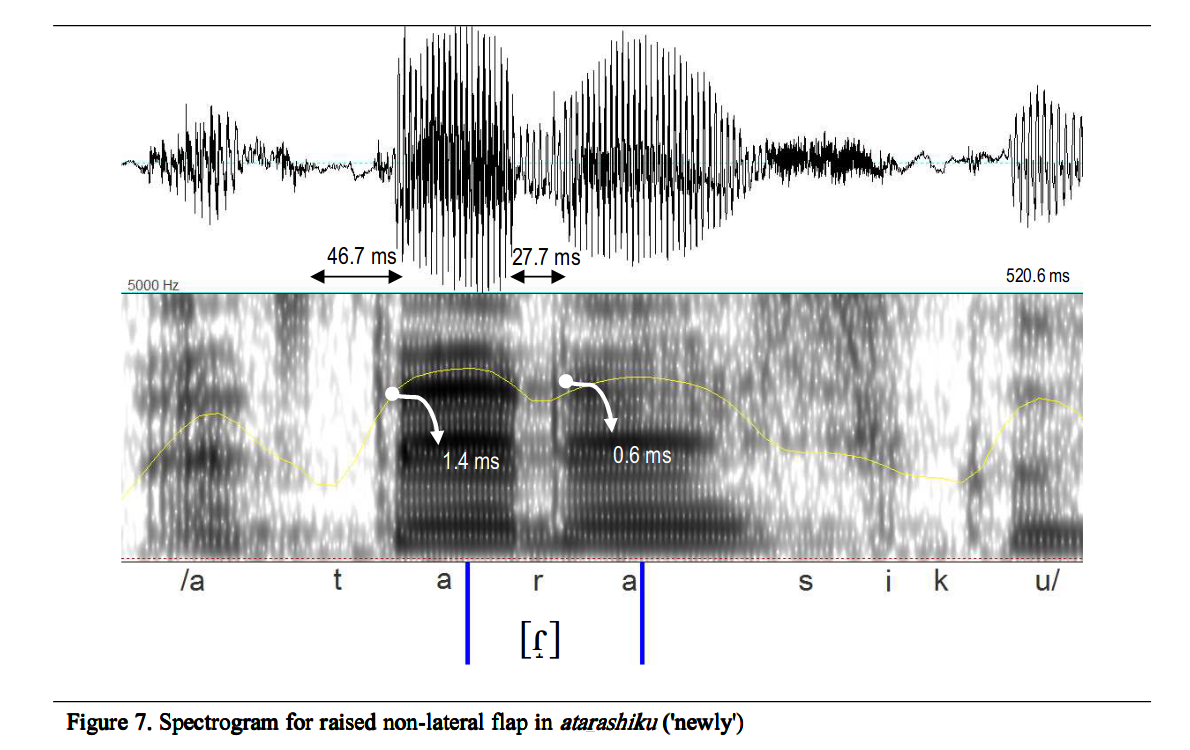
\includegraphics[width=0.8\linewidth]{substance/images/figure7_magnuson}
	\caption[Illustration du  ɾ̝  par \textcite{magnusonWhatSoundsKansai2008}]{Illustration du  ɾ̝  par \textcite[p.61]{magnusonWhatSoundsKansai2008} avec un oscillogramme en haut, et un spectrogramme en bas. La durée du /t/ est de 46,7 ms dont 1,4 ms pour la phase de relâchement contre une durée de 27,7 ms pour le /r/ dont 0,6 ms pour la phase de relâchement.}
	\label{fig:figure7magnuson}
\end{figure}

Nous avons choisi de ne pas adopter cette méthodologie pour les langues sur lesquelles nous travaillons. En effet, cette méthodologie est chronophage et implique une vision globale des données, comme \citeauthor{sebregtsSociophoneticsPhonologyDutch2014} l'indique dès le début de sa thèse dans ses remerciements : \textg{[...] that process was a laborious one of defining and redefining categories, listening and relistening and re-relistening to thousands of tokens.} (p. xi). Elle demande aussi, quand c'est possible, d'avoir plusieurs transcripteurs, ou de revenir a posteriori sur les annotations (ici un mois plus tard) comme \textcite{magnusonWhatSoundsKansai2008} l'a fait car il était seul face à ses données, et ce, afin de mesurer sa cohérence. Notre but principal n'étant pas de mesurer la variation de la rhotique, nous avons fait le choix de ne suivre ni la méthode d'annotation a posteriori de \textcite{magnusonWhatSoundsKansai2008} ni de demander à une deuxième personne de transcrire et d'annoter avec nous.


\subsection{Travaux sur la base de catégories plus larges : le malayalam et le persan}

Le malayalam contraste au moins deux rhotiques qui peuvent être décrites soit comme étant une opposition entre un trill et un tap, soit comme deux trills avec le lieu d'articulation les contrastant. L'\textit{Illustration of the IPA} \cite{namboodiripadMalayalamNamboodiriDialect2017a} sur le dialecte namboodiri du malayalam fait état d'une opposition entre un segment trill /r/ et un segment tap or flap /ɾ/. On retrouve également dans l'inventaire une approximante rétroflexe /ɻ/.\\

\citeauthor{punnooseAuditoryAcousticStudy2010} a identifié seulement cinq variants différents dans sa thèse. Il s'agit des segments suivants :

\begin{itemize}
	\item Le tap approximant
	\item Le trill approximant
	\item Le tap canonique
	\item La séquence trill + voyelle épenthétique
	\item Le trill multi-contacts
\end{itemize}

Lors de ses recherches en socio-phonétique sur le persan, \textcite{rafatSocioPhoneticInvestigationRhotics2010} code quatre catégories. Son étude inclut deux locuteurs et trois locutrices tous/toutes titulaires (ou en cours d'obtention) d'un diplôme de l'éducation supérieure. Les catégories sont utiles pour classer les rhotiques des mots issus d'une tâche de lecture de mot, et une tâche de mémorisation de mots, censée être plus spontanée. Dans son étude, le trill est caractérisé par des phases d'ouvertures et de fermetures présentes sur un spectrogramme à bandes larges; le tap n'est pas décrit; la fricative est caractérisée par l'absence de structure formantique et la présence de bruit; et l'approximante est caractérisée par une structure formantique et un signal périodique.\\


Il est important de faire le lien entre deux types de méthodologie. D'un côté, on retrouve la méthodologie de \textcite{blecuaVibrantesEspanolManifestaciones2002} qui s'intéresse à la composition des trills et des taps. De l'autre côté, l'important est l'élaboration de catégories sur la base de motifs acoustiques. En effet, on retrouve les symboles API avec \textcite{sebregtsSociophoneticsPhonologyDutch2014} pour le néerlandais, \textcite{patinWashiliShingazidja2013} pour le washili shingazidjan (non développé ici) ou encore \textcite{magnusonWhatSoundsKansai2008} pour le japonais. Et on retrouve des catégories sans aucun symbole avec \textcite{rafatSocioPhoneticInvestigationRhotics2010} pour le perse ou \citeauthor{punnooseAuditoryAcousticStudy2010} pour le malayalam.\\

Nous pensons que l'intégration des différentes méthodologies permet une meilleure compréhension de la distribution typologique du trill et du tap : d'un côté nous aurions des catégories qui seraient similaires à celles qu'on pourrait avoir en phonétique segmentale, et d'un autre la substance pouvant être incluse dans ces catégories. Cette substance pourrait être comparée à des gestes articulatoires.


\section{Première étude : classification des trills et taps dans des macro-classes}

\subsection{Quatre catégories différentes}

Nous avons parcouru tous les enregistrements sonores des narratives des \textit{illustrations of the IPA}. Nous avons eu accès à 81 enregistrements pour 75 langues. Pour certaines illustrations plusieurs personnes pouvaient être enregistrées.\\

Nous avons fait le choix, dès le début, d'opter pour une annotation sans symbole API. Ces catégories sont similaires à celles adoptées par \textcite{rafatSocioPhoneticInvestigationRhotics2010} car suffisamment larges pour permettre la catégorisation d'un maximum de réalisations des rhotiques, tout en ciblant les productions à plusieurs occlusions.
Ainsi, nous avons commencé notre annotation par quatre catégories : \textg{t1}, \textg{t2}, \textg{t3} et \textg{t4}.\\

La catégorie \textg{t1} fait référence à un segment à une occlusion courte (\autoref{fig:haus125777110}). Au niveau du spectrogramme, on retrouve une zone d'énergie moins importante qui s'observe au niveau du signal par une baisse de l'amplitude et de l'intensité du signal.\\

\begin{figure}
	\centering
	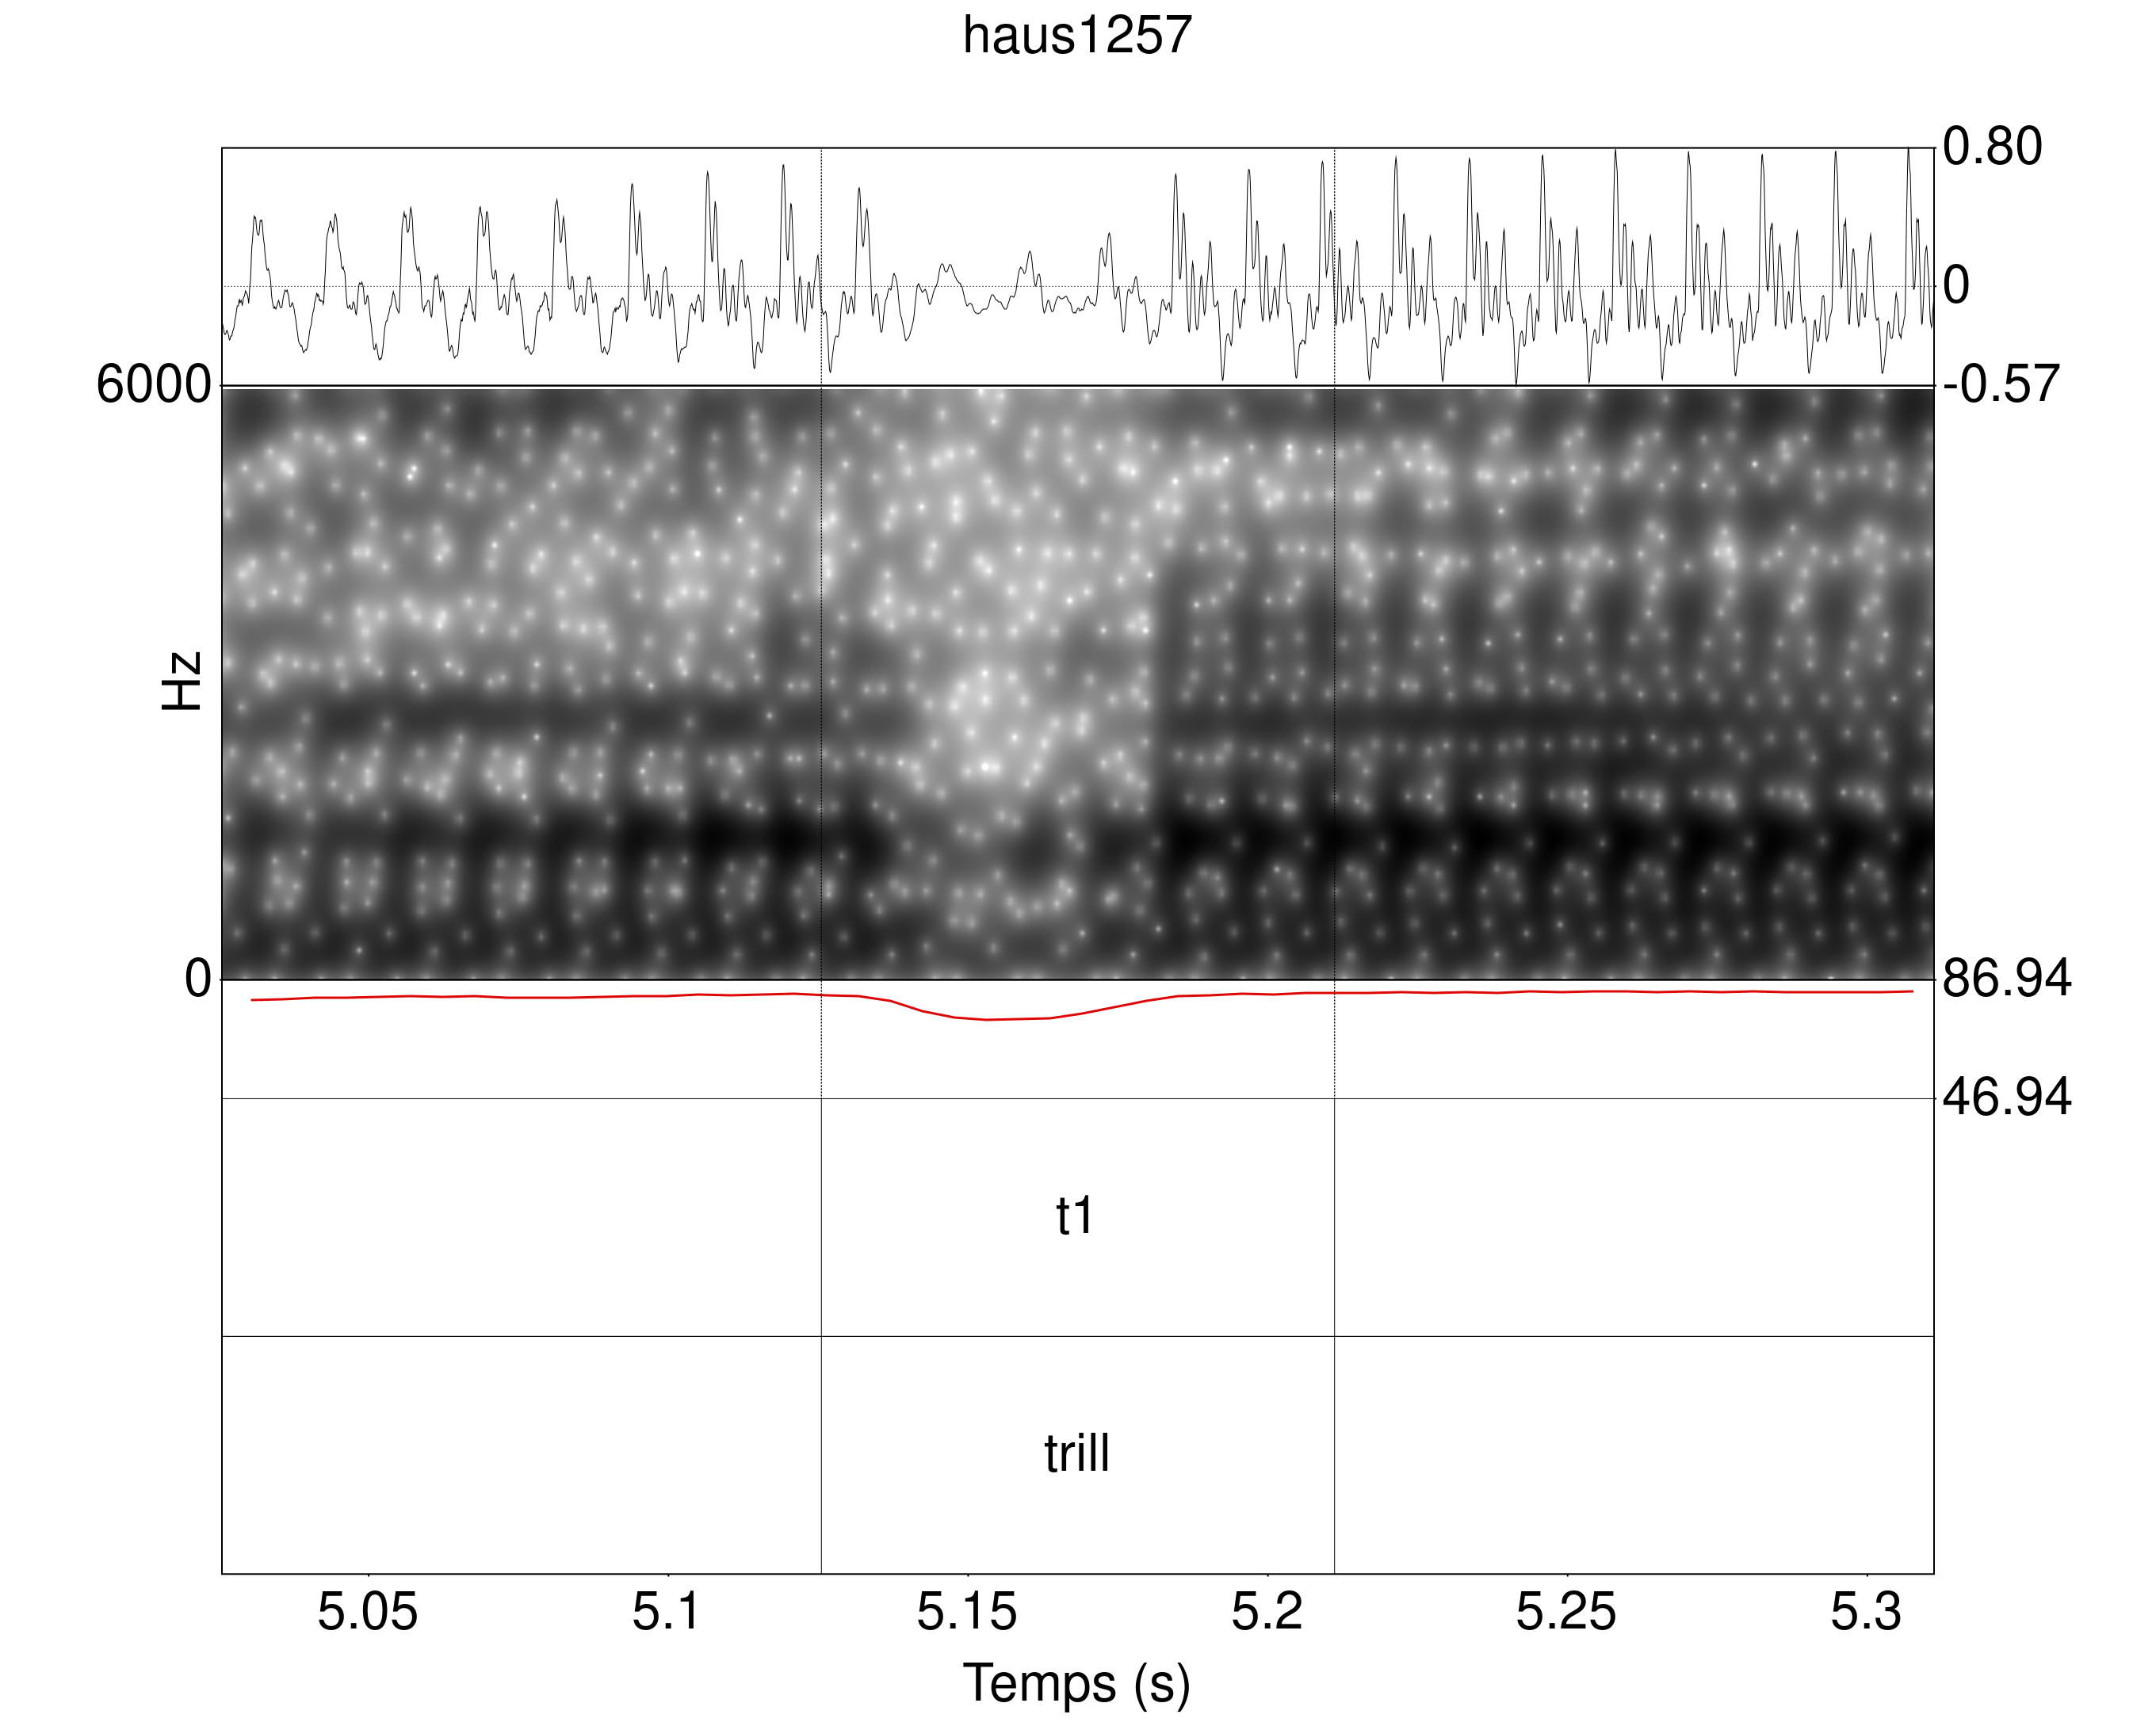
\includegraphics[width=0.8\linewidth]{substance/spectro_images/haus1257_768_4}
	\caption[Illustration de la catégorie \textg{t1}]{Illustration de la catégorie \textg{t1} dans le contexte [wɘtɘ raːnaː] en hausa \glotto{haus1257}. De haut en bas, nous avons l'oscillogramme, le spectrogramme, la courbe d'intensité, un palier intervallique avec la catégorie segmentée, et un palier intervallique comprenant le label descriptif du segment d'intérêt.}
	\label{fig:haus125777110}
\end{figure}


La catégorie \textg{t2} fait référence à un segment à au moins deux occlusions (\autoref{fig:nenn1238131256}), au moins deux diminutions de l'intensité et donc de l'amplitude du signal.\\

\begin{figure}
	\centering
	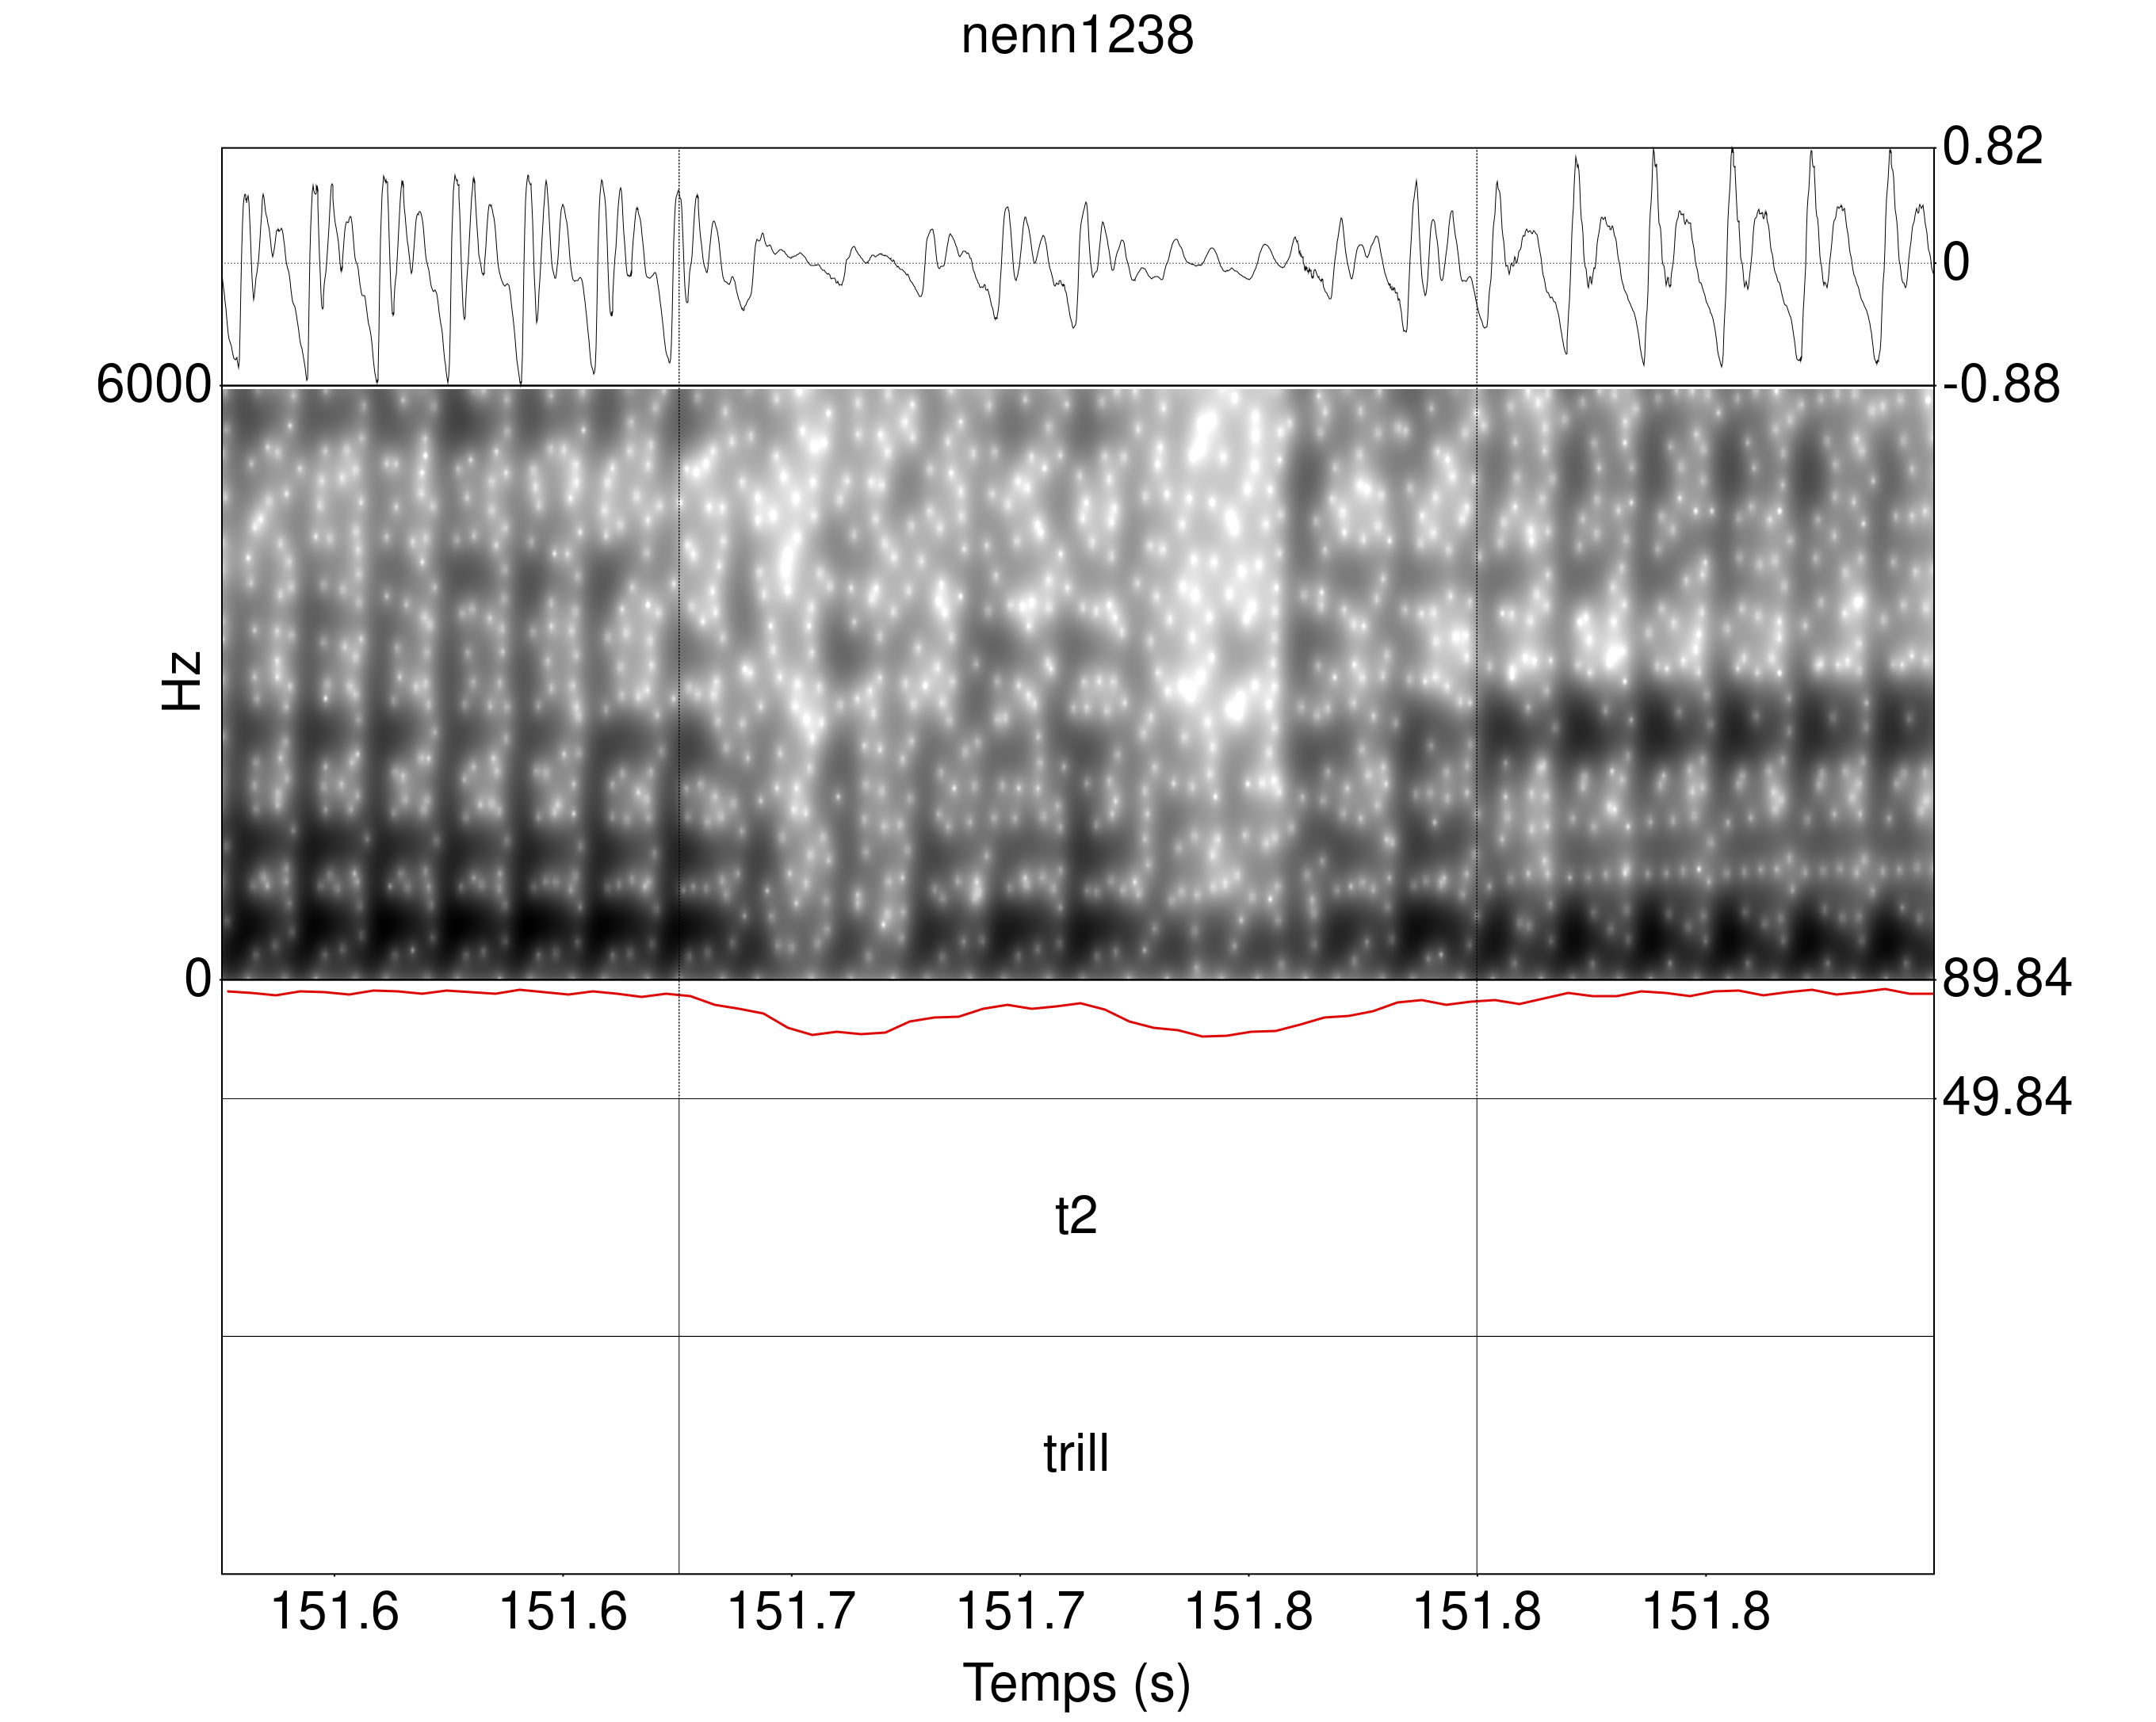
\includegraphics[width=0.8\linewidth]{substance/spectro_images/nenn1238_1312_56}
	\caption[Illustration de la catégorie \textg{t2}]{Illustration de la catégorie \textg{t2} dans le contexte [ˈkesær ˈombtebas] en nen \glotto{nenn1238}. De haut en bas, nous avons l'oscillogramme, le spectrogramme, la courbe d'intensité, un palier intervallique avec la catégorie segmentée, et un palier intervallique comprenant le label descriptif du segment d'intérêt.}
	\label{fig:nenn1238131256}
\end{figure}

La catégorie \textg{t3} fait référence à un segment contenant du bruit similaire à celui qu'on retrouve dans les fricatives.\\

\begin{figure}
	\centering
	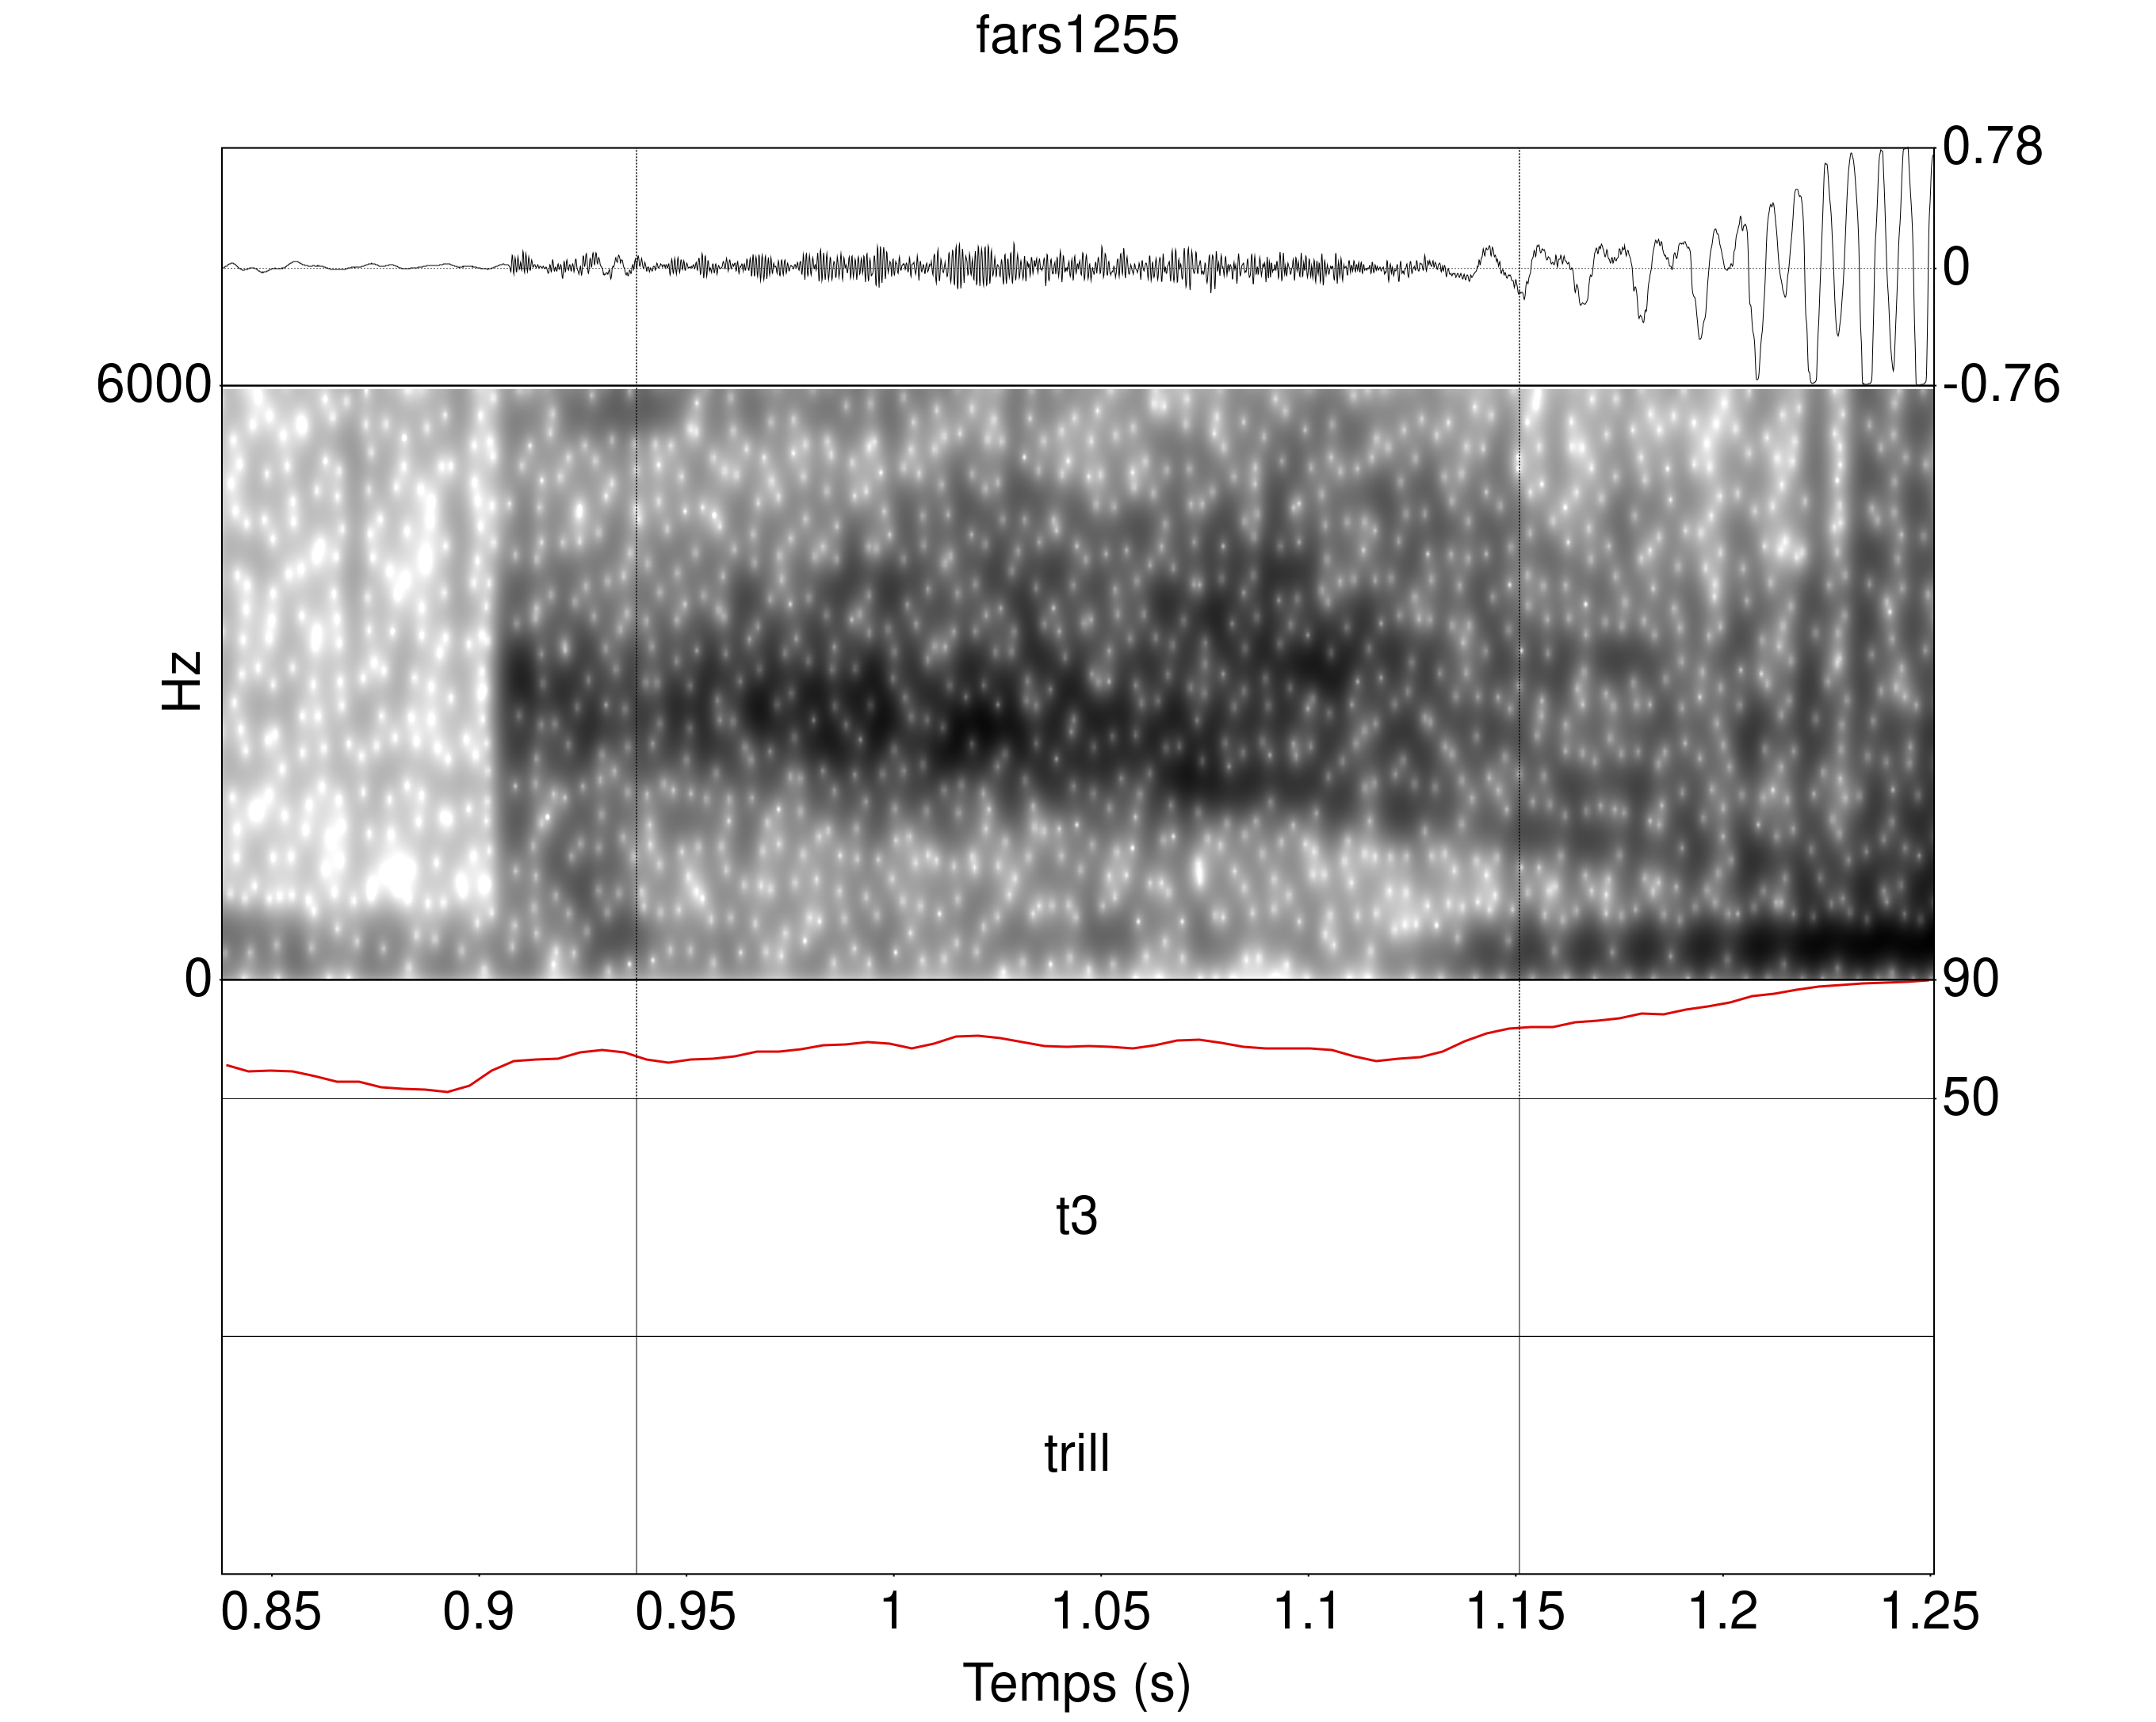
\includegraphics[width=0.8\linewidth]{substance/spectro_images/fars1255_449_2}
	\caption[Illustration de la catégorie \textg{t3}]{Illustration de la catégorie \textg{t3} dans le contexte [ˈjet ˈruzi] en farsi \glotto{fars1255}. De haut en bas, nous avons l'oscillogramme, le spectrogramme, la courbe d'intensité, un palier intervallique avec la catégorie segmentée, et un palier intervallique comprenant le label descriptif du segment d'intérêt.}
	\label{fig:fars12554492}
\end{figure}


La catégorie \textg{t4} fait référence à tout le reste, il s'agit d'une catégorie où on retrouve principalement des approximantes.\\

\begin{figure}
	\centering
	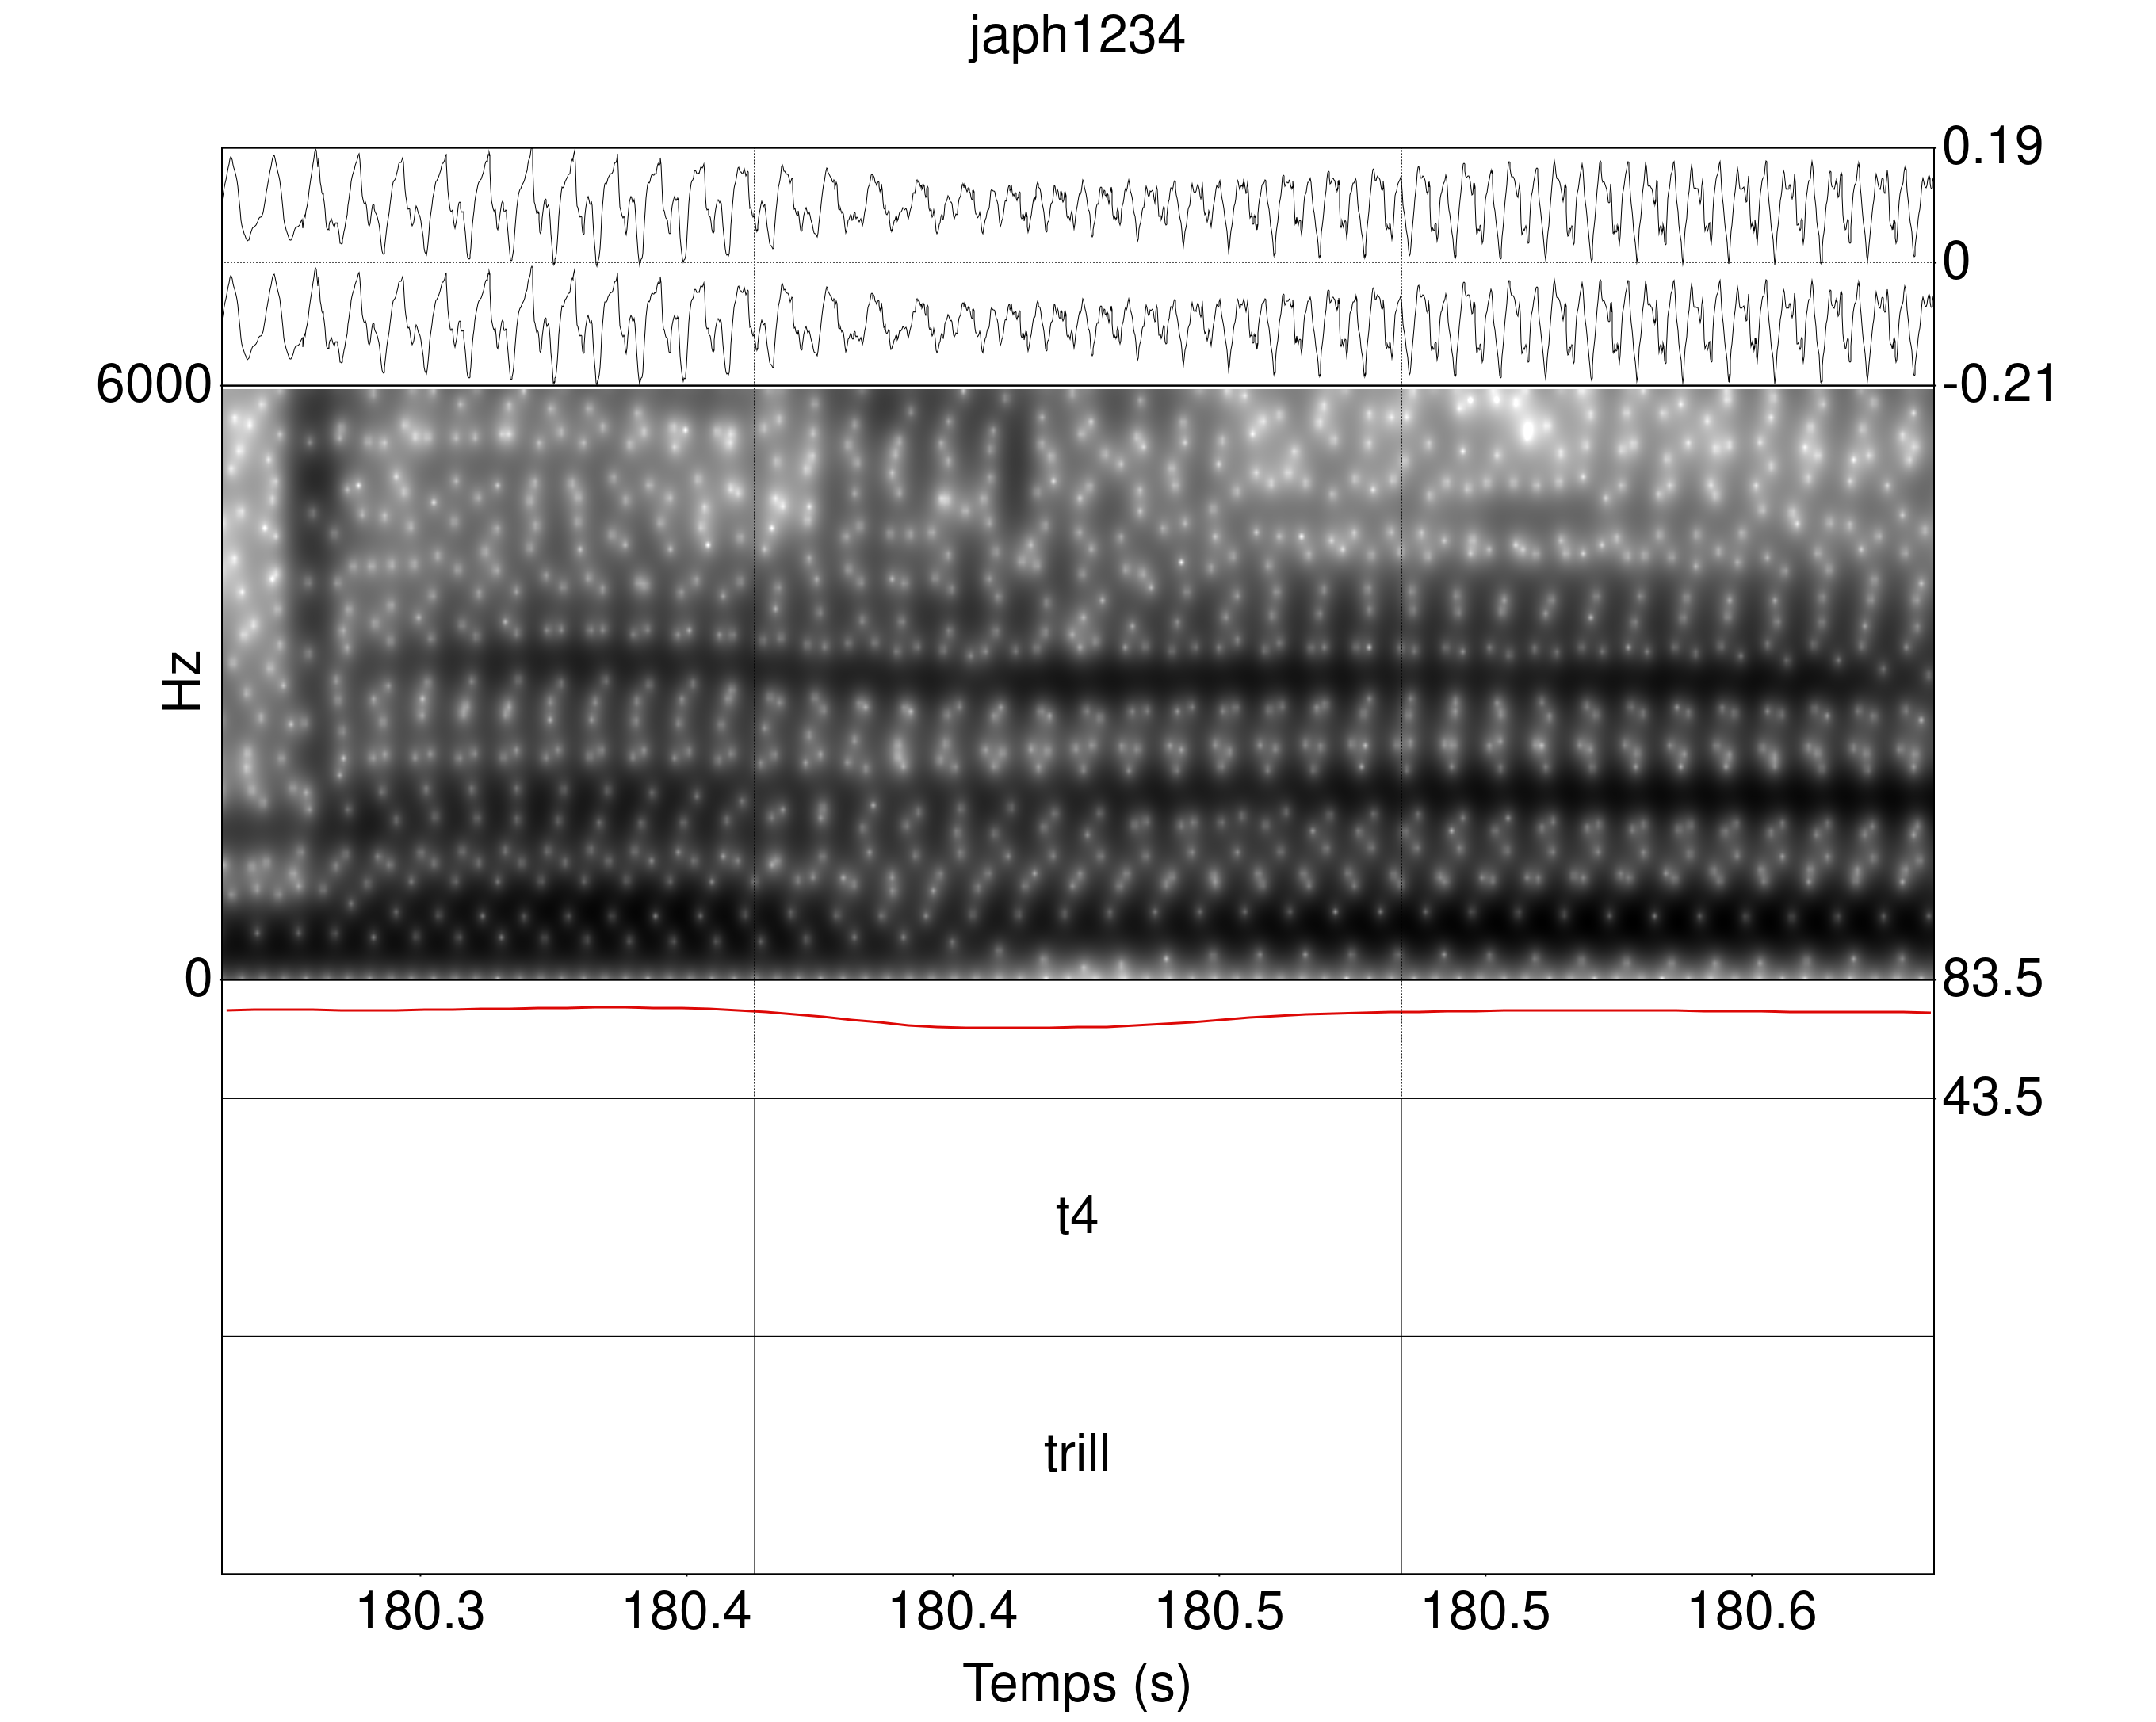
\includegraphics[width=0.8\linewidth]{substance/spectro_images/japh1234_944_70}
	\caption[Illustration de la catégorie \textg{t4}]{Illustration de la catégorie \textg{t4} dans le contexte /tɕendɤre/ en japhug \glotto{japh1234}. De haut en bas, nous avons l'oscillogramme, le spectrogramme, la courbe d'intensité, un palier intervallique avec la catégorie segmentée, et un palier intervallique comprenant le label descriptif du segment d'intérêt.}
	\label{fig:japh123494470}
\end{figure}

De plus, nous avons ajouté deux autres catégories (\autoref{fig:taus_mono}) : \textg{t5}, faisant référence à un segment avec une occlusion qui visuellement semble plus longue que celle d'un segment classé comme t1. Perceptuellement, le segment ressemble à une occlusive. La catégorie \textg{t6} fait référence à un segment avec plus de 5-6 contacts.\\

\begin{figure}
	\centering
	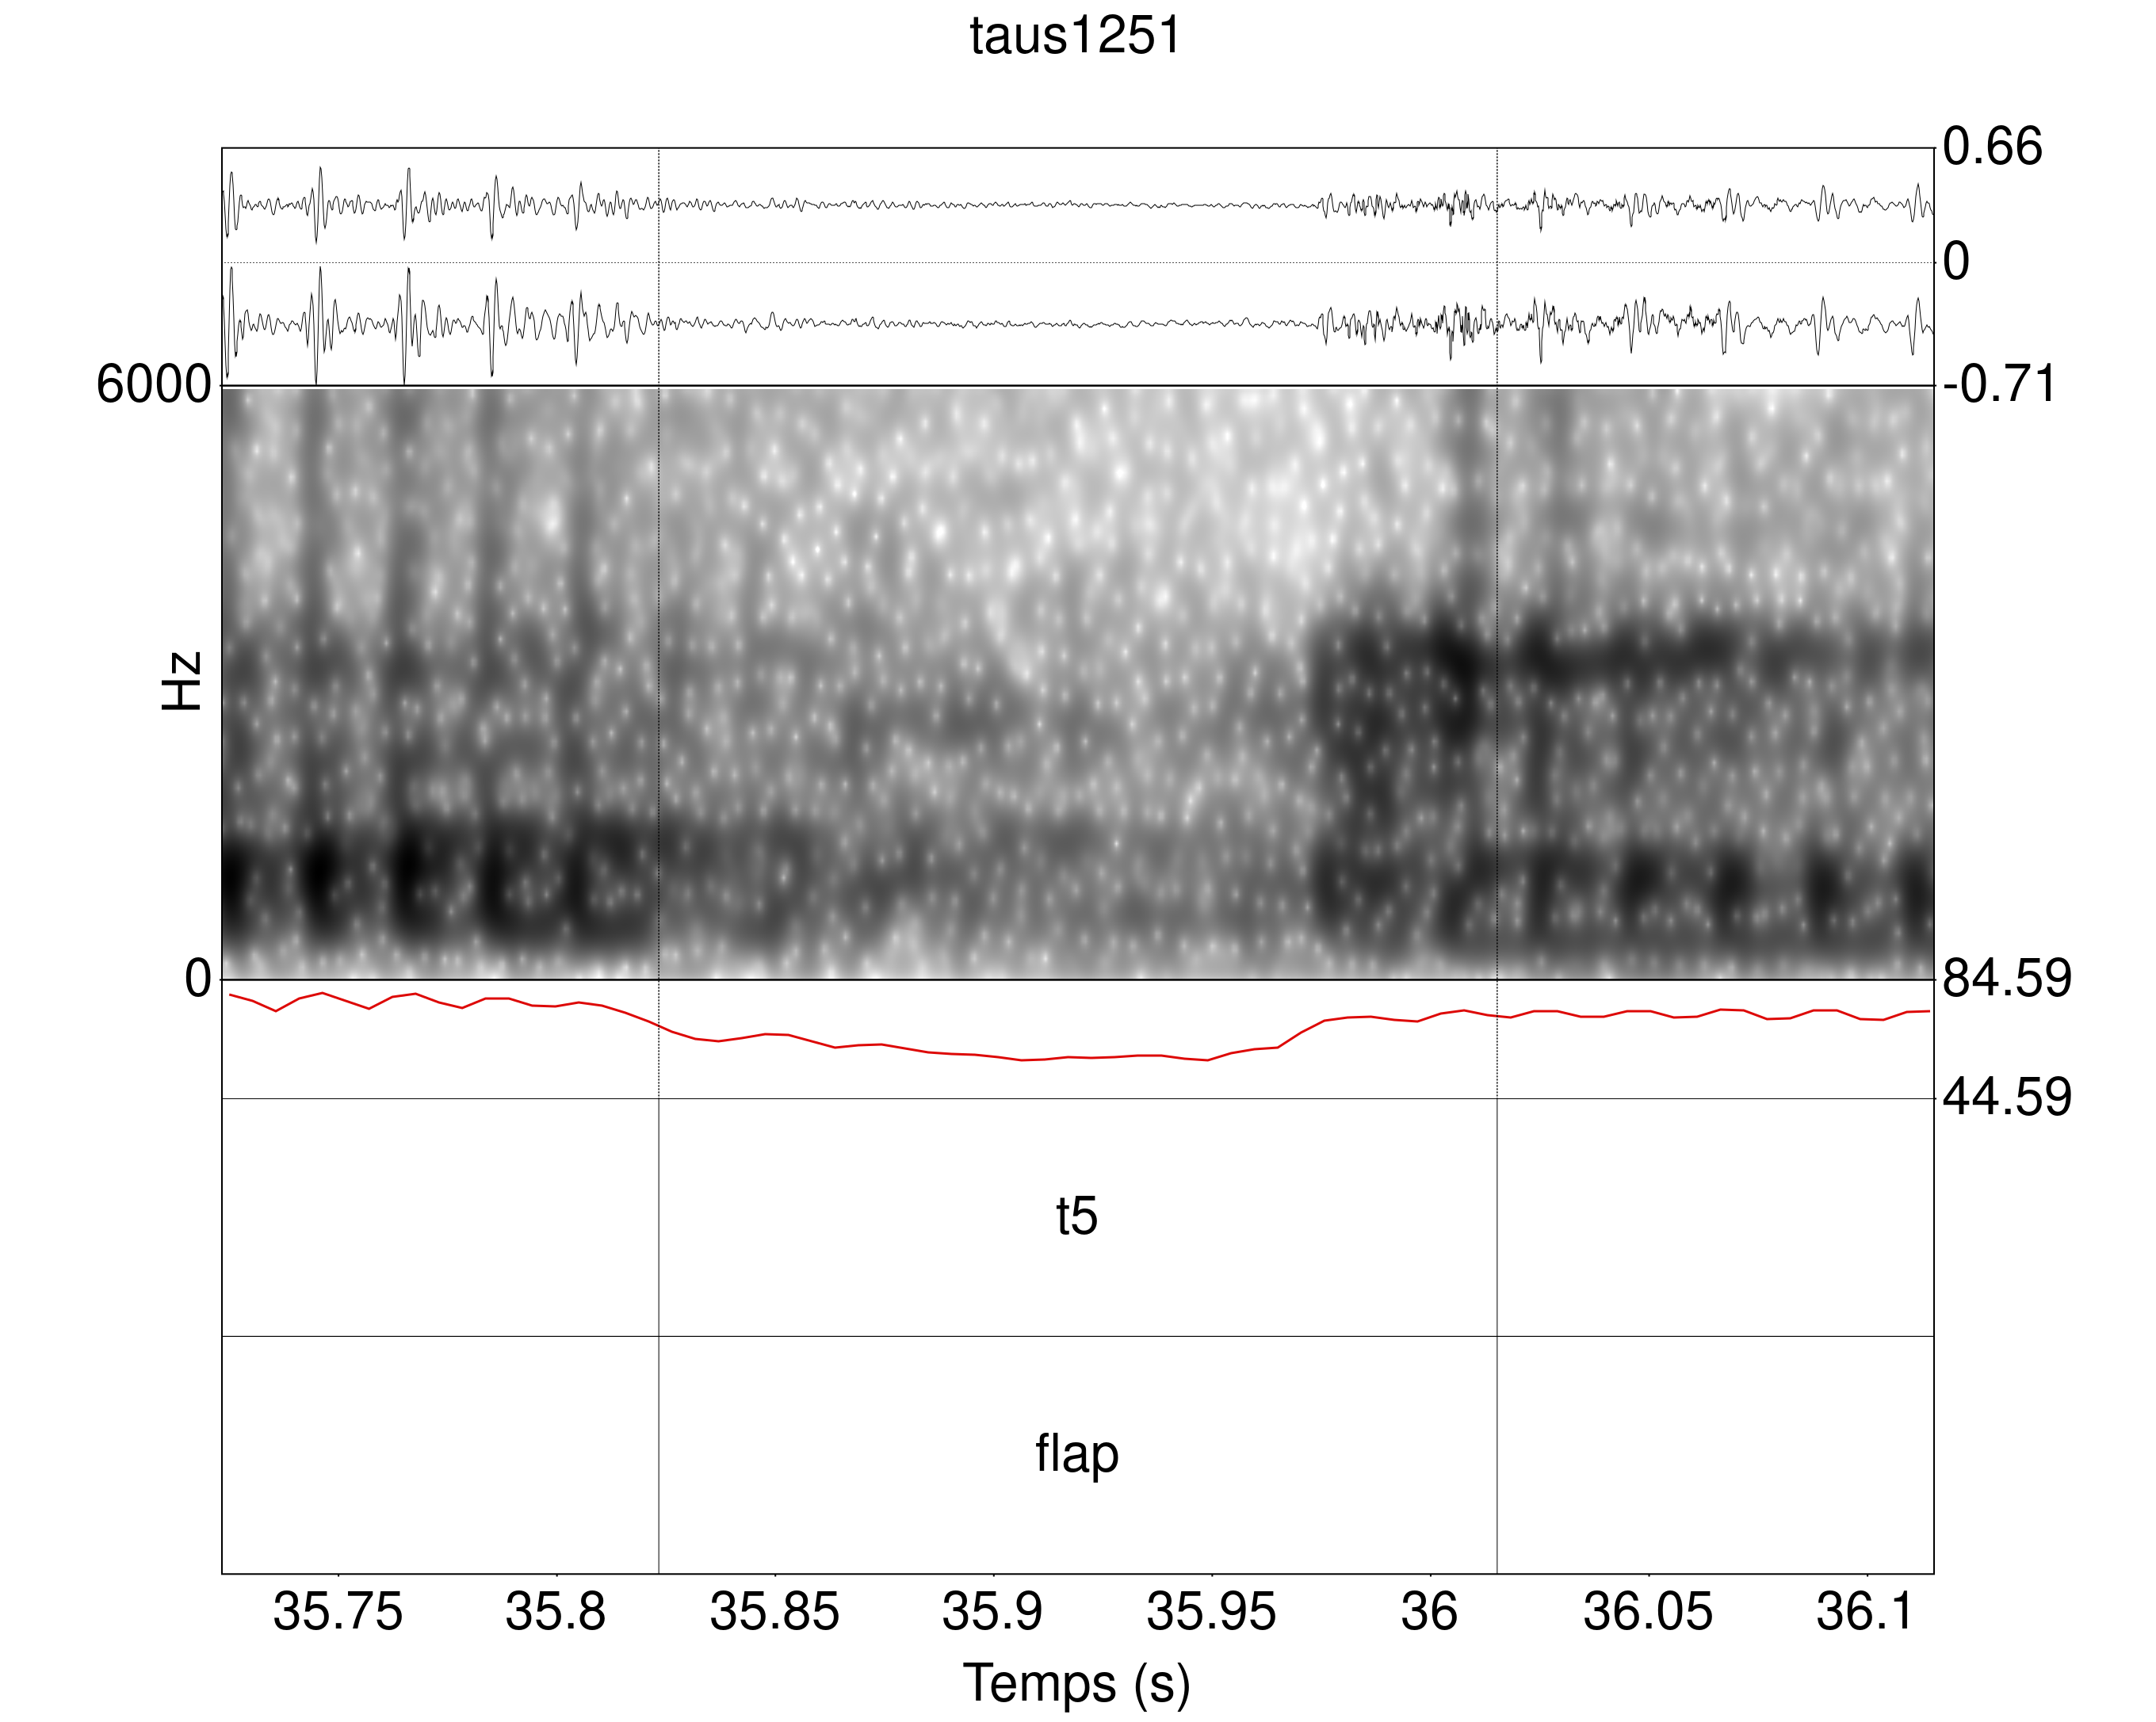
\includegraphics[width=0.45\linewidth]{substance/spectro_images/taus1251_1657_10}
	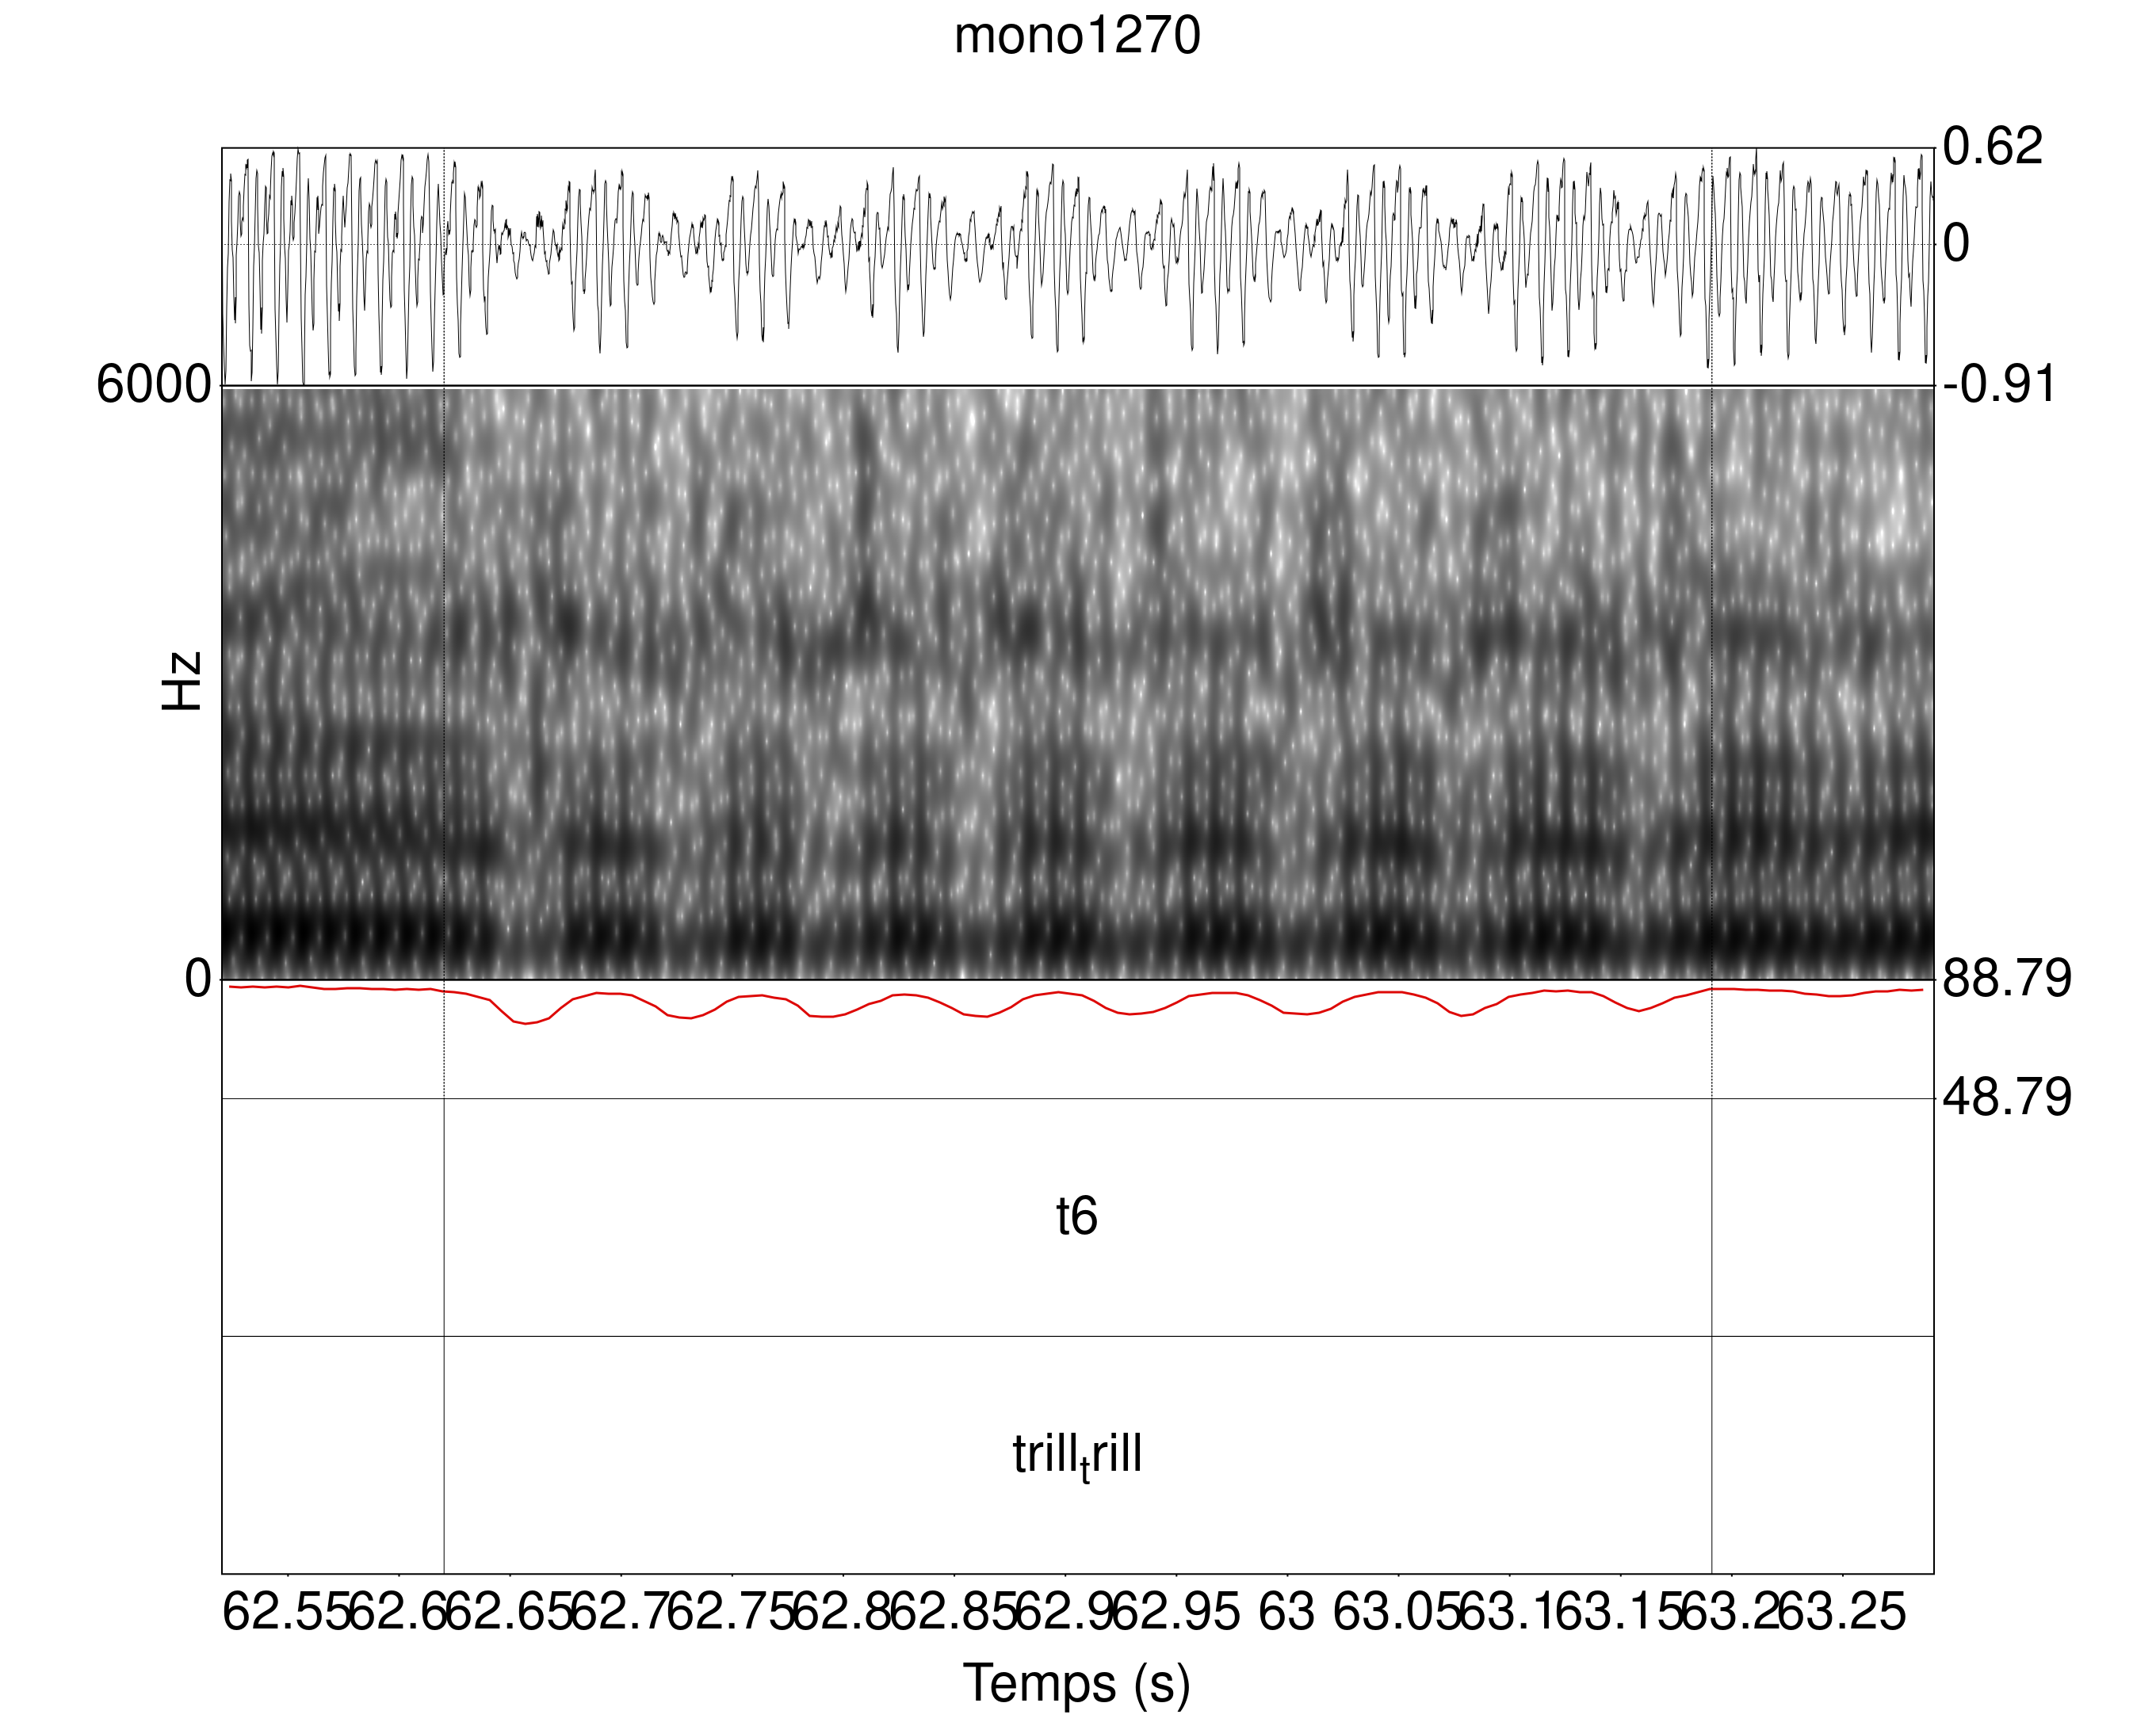
\includegraphics[width=0.45\linewidth]{substance/spectro_images/mono1270_1188_12}
	\caption[Illustrations des catégories \textg{t5} et \textg{t6}]{Illustration de la catégorie \textg{t5} dans le contexte [haˈɾuwa] en tausug (à gauche) et illustration de la catégorie \textg{t6} dans le contexte [ə́rː jìgú] <Œrrrœ yigu> en mono (à droite). De haut en bas pour chacune des illustrations, nous avons l'oscillogramme, le spectrogramme, la courbe d'intensité, un palier intervallique avec la catégorie segmentée, et un palier intervallique comprenant le label descriptif du segment d'intérêt.}
	\label{fig:taus_mono}
\end{figure}

\subsection{Résultats de la segmentation en catégories}

\begin{table}
	\centering
	%\resizebox{0.7\linewidth}{!}{\csvautobooktabular{substance/tables/table_elements_diff.csv}}
	\resizebox{\linewidth}{!}{


\begin{tabular}{p{4.5cm} l  || p{4.5cm} l}
\hline
Label descriptif	&	Fréquence	&	Label descriptif	&	Fréquence	\\
\hline
Trill	&	1117	&	Trill géminé	&	9	\\
Tap	&	434	&	Tap rétroflexe	&	6	\\
Trill/tap	&	54	&	Trill uvulaire	&	6	\\
Trill/flap	&	28	&	Trill non voisé	&	4	\\
Stop	&	22	&	Tap non voisé	&	3	\\
Tap/flap	&	22	&	Trill/fricative	&	3	\\
Flap	&	20	&	Trill rétroflexe	&	2	\\
Approximante rétroflexe	&	19	&	Trill syllabique	&	2	\\
Trill palatalisé	&	13	&	Approximante	&	1	\\
Stop non voisé	&	8	&	Liquide latérale	&	1	\\
Trill/flap rétroflexe	&	8	&	Trill glottalisé	&	1	\\

\hline
\end{tabular}
}
	\caption[Fréquence des différents labels descriptifs utilisés dans les \textit{Illustrations of the IPA} pour les rhotiques]{Fréquence des différents labels descriptifs utilisés dans les \textit{Illustrations of the IPA} pour les rhotiques.}
	\label{tab:table_descLabel}
\end{table}

La segmentation et l'annotation des différents segments se sont faites sur une période s'étalant sur trois mois. Nous nous sommes appuyés sur les transcriptions déjà établies dans les \textit{illustrations of the IPA}.
Au total, ce sont 1783 segments qui ont été segmentés et annotés pour 22 labels descriptifs (cf. \autoref{tab:table_descLabel}). Nous définissons ici le label descriptif comme la manière utilisée par les auteurs des différentes illustrations pour se référer à un segment.
Ainsi, un auteur peut parler d'un "r" comme étant, par exemple, un flap, un trill ou encore une approximante. Par défaut, les labels descriptifs référent à des segments produits au niveau alvéolaire. D'une part, nous avons les labels descriptifs appartenant au domaine de l'analyse linguistique, et de l'autre, les différentes catégories qui relèvent des motifs issus de l'interprétation du signal acoustique. Le signal acoustique motive les catégories, et non les labels descriptifs.
De plus, un segment qui ne possède qu'un label descriptif peut appartenir à plusieurs catégories en fonction de sa réalisation.\\

Nous avons fait le choix de ne pas inclure tous les labels descriptifs dans notre échantillon final. Nous n'avons gardé que les labels descriptifs des \textg{trill}, \textg{tap}, \textg{trill/tap}, \textg{trill/flap}, \textg{tap/flap} et \textg{flap} et les catégories \textg{t1}, \textg{t2}, \textg{t3} et \textg{t4}.
Notre échantillon final comporte les productions de 73 langues, soit au total 79 locuteurs et locutrices pour 1672 segments.\\


\begin{figure}
	\centering
	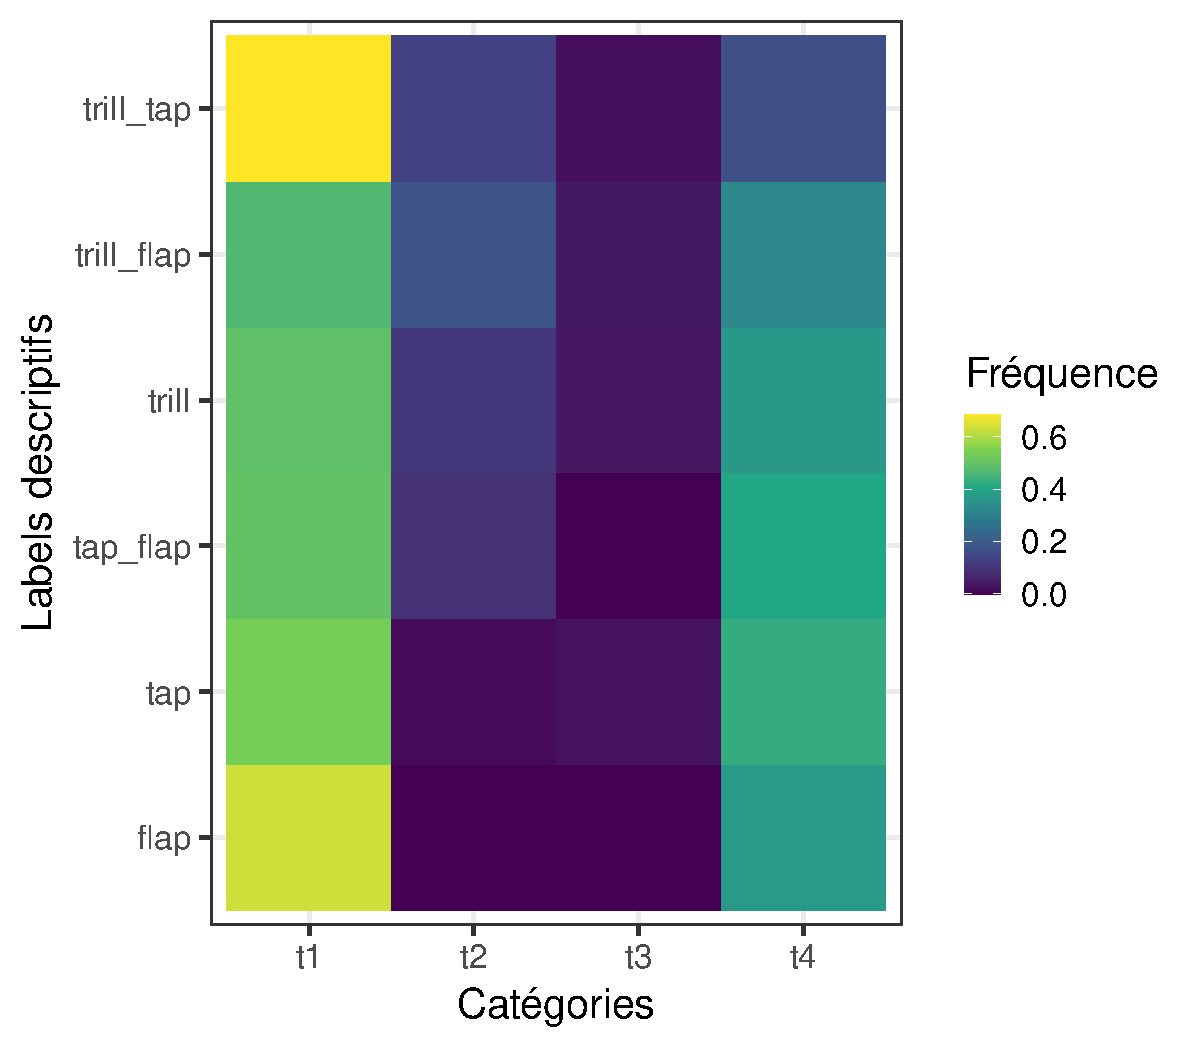
\includegraphics[width=0.45\linewidth]{substance/images/categories_full}
	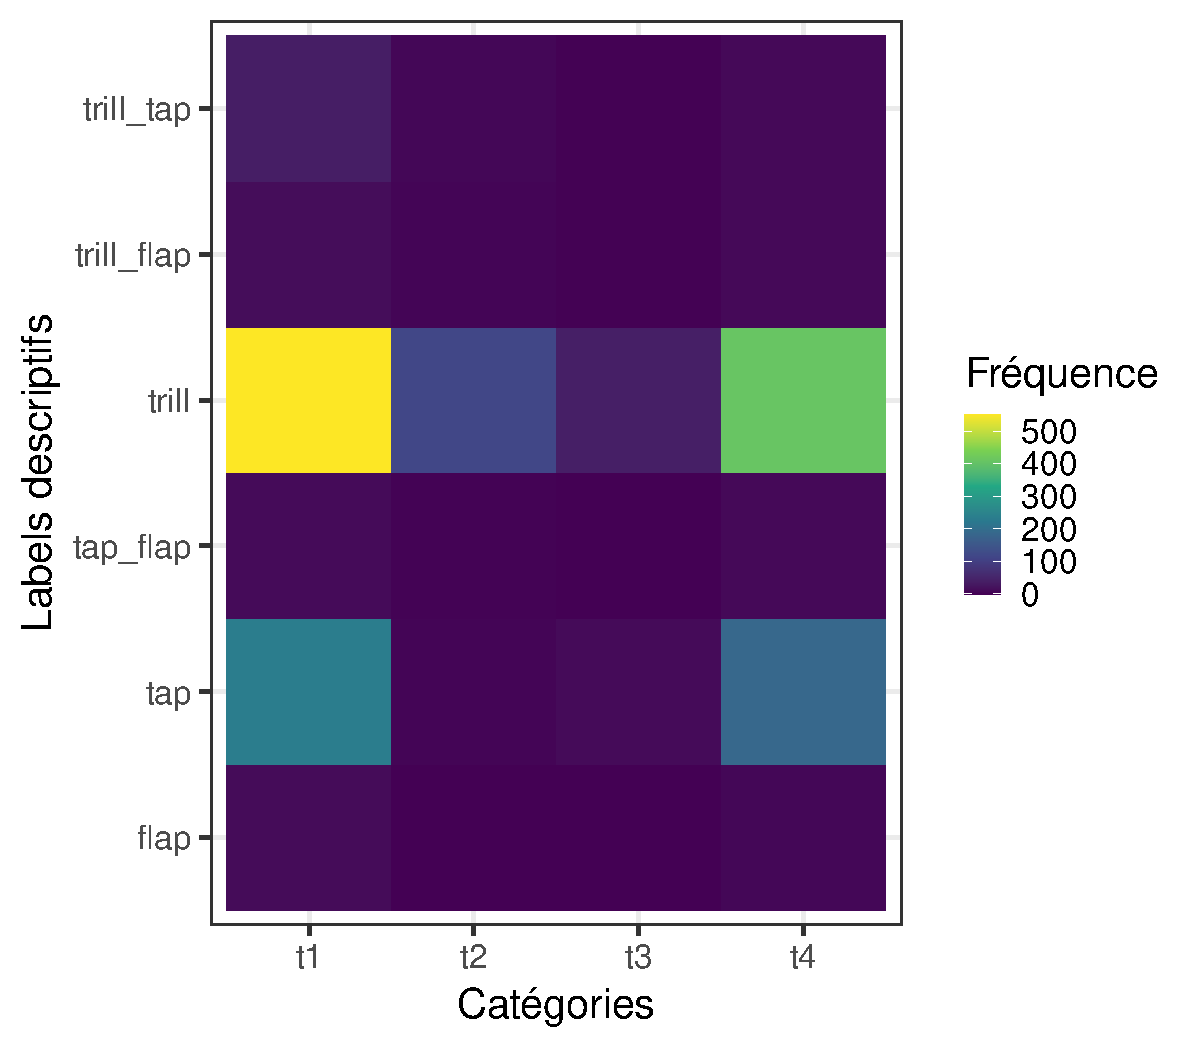
\includegraphics[width=0.45\linewidth]{substance/images/categories_full_freqabs}
	\caption[Fréquences des différentes catégories en fonction des labels descriptifs]{Fréquences relatives (à gauche) et fréquences absolues (à droite) des différentes catégories en fonction des labels descriptifs. Les fréquences sont calculées par ligne. Plus une case est jaune, plus la catégorie associée à un label descriptif est fréquente. Plus une case est violette, moins la catégorie associée à un label descriptif est fréquente.}
	\label{fig:categoriesfull}
\end{figure}

Lorsqu'on regarde les labels descriptifs, les trills sont les segments les plus fréquents dans nos données. Les trills représentent 67\% de toutes les rhotiques segmentées. Les taps représentent 26\% des données. Les trills/taps, trills/flaps, taps/flaps et flaps se partagent les 7\% restants.
La plupart des segments ont été catégorisés comme des \textg{t1} et des \textg{t4} (\autoref{fig:categoriesfull}). La catégorie \textg{t2} n'est jamais la plus fréquente même dans les cas où le label descriptif est \textg{trill}, autrement dit, un motif acoustique avec au moins deux occlusions n'est jamais le motif le plus fréquent dans les segments identifiés comme \textit{trill} par les auteurs des illustrations.\\

Dans la partie qui suit, nous allons nous intéresser à la variation entre les langues, en contrôlant le label descriptif utilisé par les auteurs des illustrations. Autrement dit, comme chaque langue est représentée par un locuteur ou une locutrice, nous allons observer la variation inter-locuteur.\\


Nous nous intéressons dans un premier temps au trill. En \autoref{fig:variationtrill} nous pouvons observer les données pour les 65 locuteurs/trices de langues où on retrouve des trills.
Parmi ces personnes enregistrées, seulement six ont réalisé au moins 50\% de leurs segments labellisés \textg{trill} comme des \textg{t2}, et ce chiffre augmente à huit pour les personnes en ayant réalisés au moins 40\%.
En \autoref{fig:galicastmalotswa} nous présentons les oscillogrammes, spectrogrammes et segmentations avec annotations de six de ces huit personnes. Il est intéressant de souligner que l'espagnol d'Argentine \glotto{amer1254}, le castillan \glotto{cast1244}, l'amharique \glotto{amha1245}, le galicien \glotto{gali1258} et le madurais \glotto{nucl1460} contrastent deux rhotiques dont un trill.
De plus, hormis le madurais \glotto{nucl1460} et le tamambo \glotto{malo1243}, les comptes de \textg{t2} sont inférieurs ou égaux à 3, mettant en évidence un faible nombre de productions total.
Si on regarde les fréquences absolues, 34 locuteurs/rices ont au moins un \textg{t2} comme réalisation de trills avec une moyenne à 3,44 et une médiane de 2,5 \textg{t2}.
Ainsi, 31 locuteurs/trices n'ont jamais réalisé de \textg{t2} dans leur production des trills, et seule la moitié des locuteurs/trices ont produit un \textg{t2} au moins une fois. Ce n'est donc pas parce qu'un segment est labellisé comme un trill qu'il sera réalisé comme un \textg{t2}. En outre, nous pouvons nous demander si dans une tâche de lecture de mots, ces locuteurs/trices, ne produisant pas de \textg{t2} ici, produiraient des \textg{t2}.\\


\begin{figure}
	\centering
	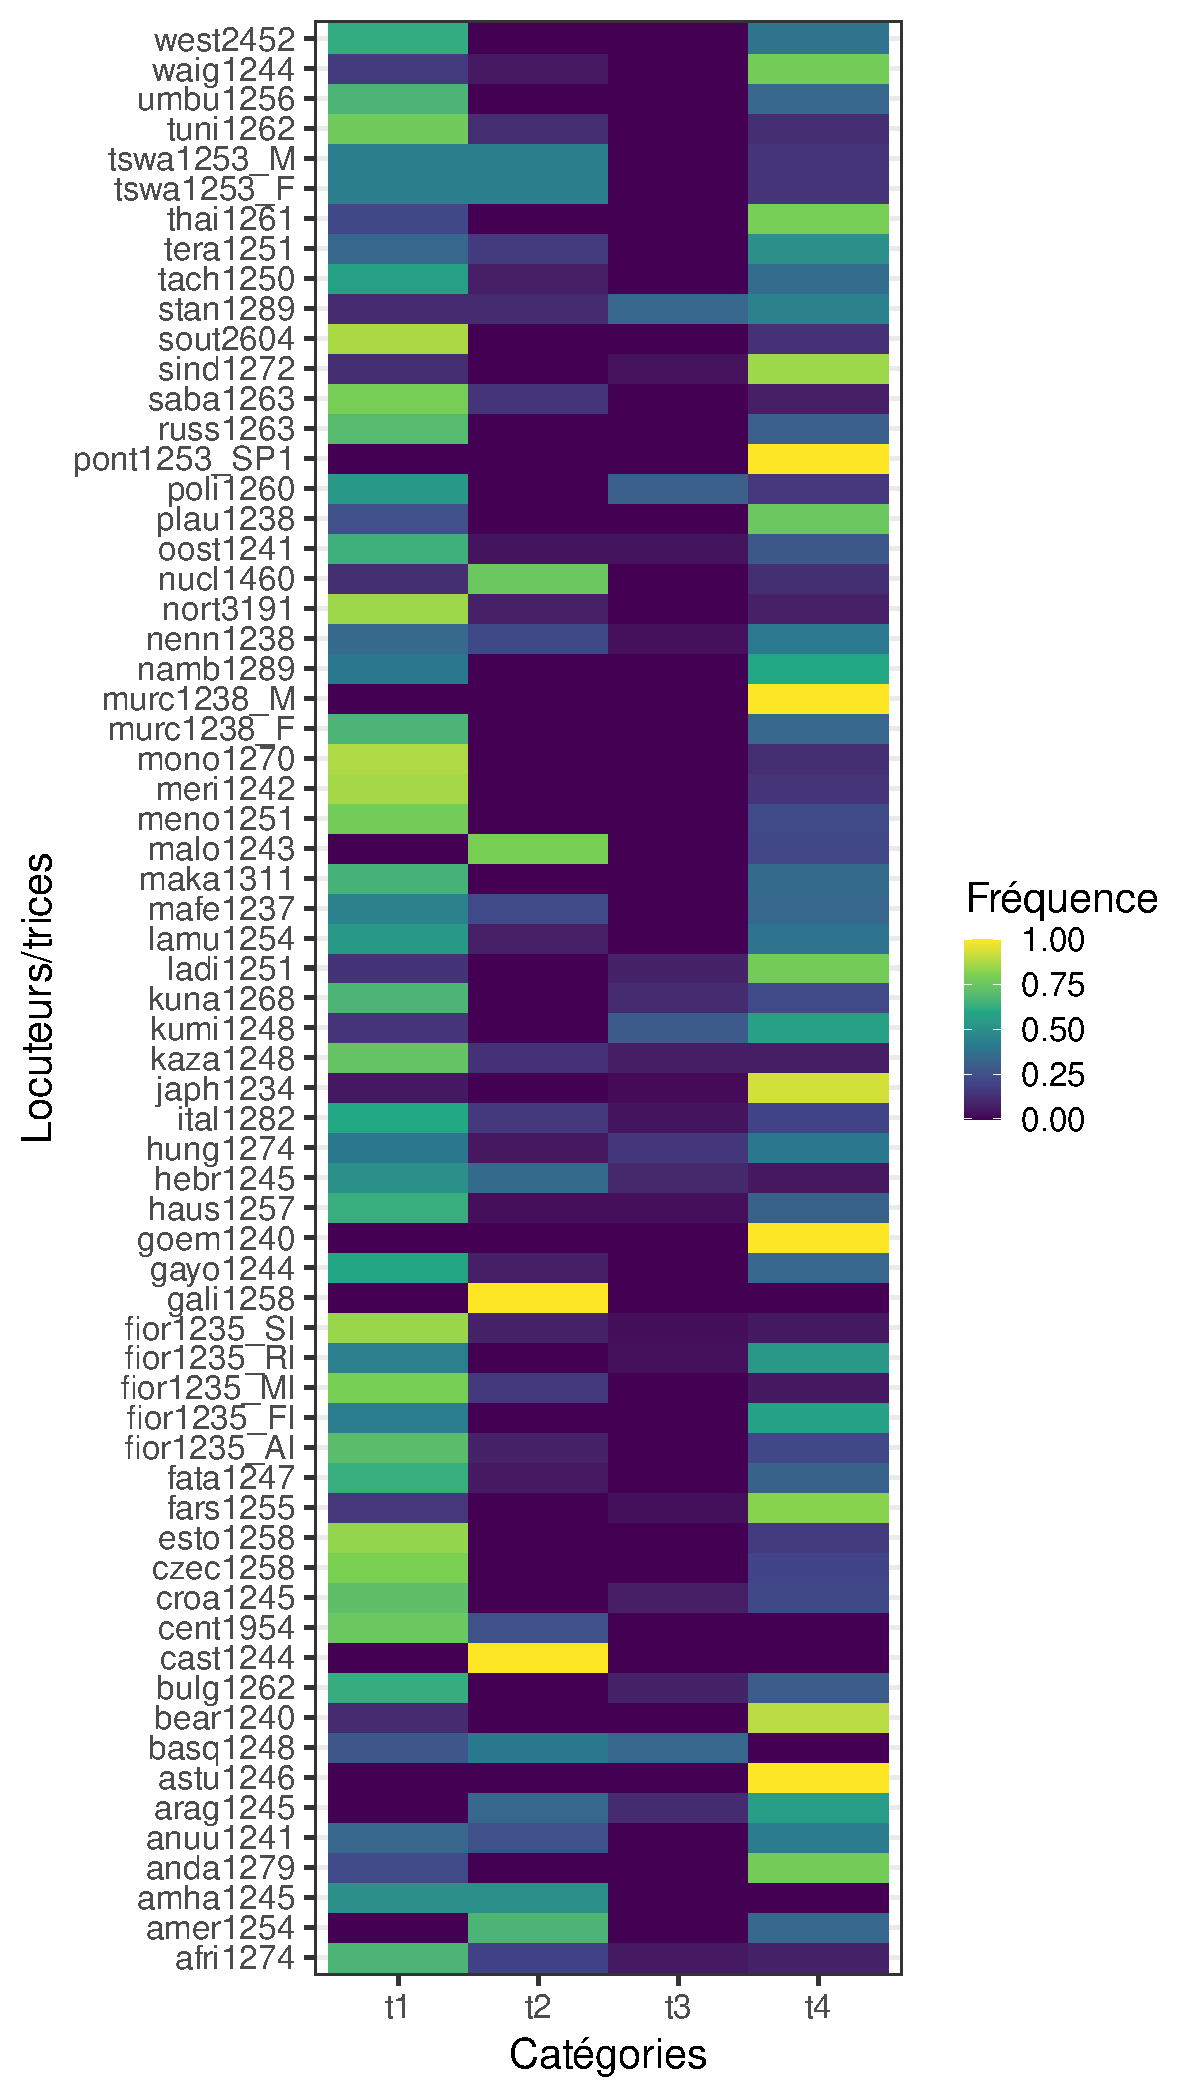
\includegraphics[width=0.45\linewidth]{substance/images/variation_trill}
	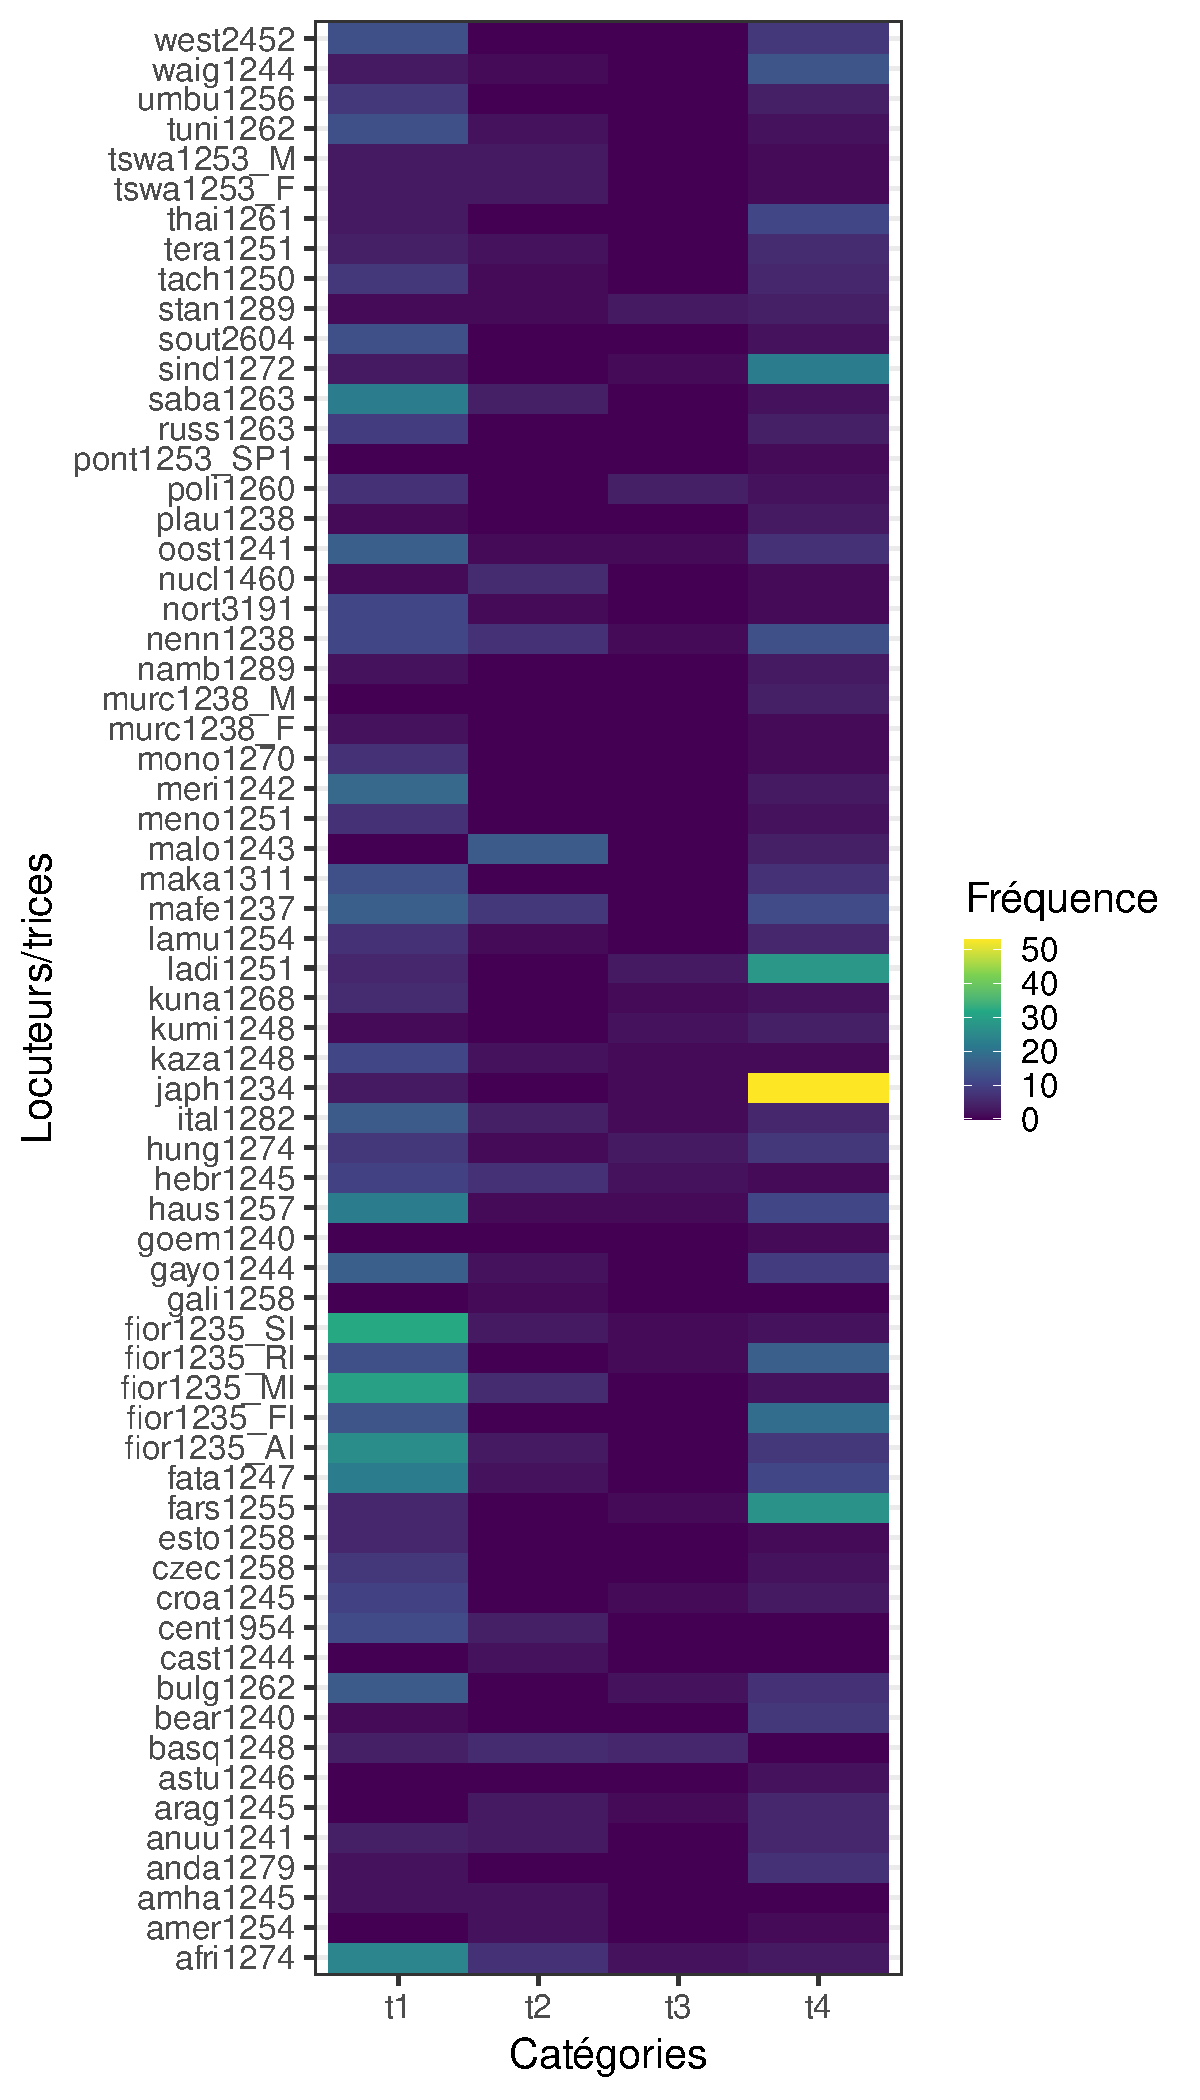
\includegraphics[width=0.45\linewidth]{substance/images/variation_trill_abs}
	\caption[Fréquences des différentes catégories illustrant la variation pour les segments ayant été catégorisés comme des \textg{trill}]{Fréquences relatives (à gauche) et absolues (à droite) des différentes catégories illustrant la variation pour les segments ayant été catégorisés par les auteurs des illustrations comme des \textg{trill}. Les fréquences sont calculées par ligne. Une case jaune est associée à une haute fréquence, cela veut dire que le/la locuteur/trice tend à produire une seule catégorie. Une case violette est associée à une catégorie non produite par le/la locuteur/trice.}
	\label{fig:variationtrill}
\end{figure}


\begin{figure}
	\centering
	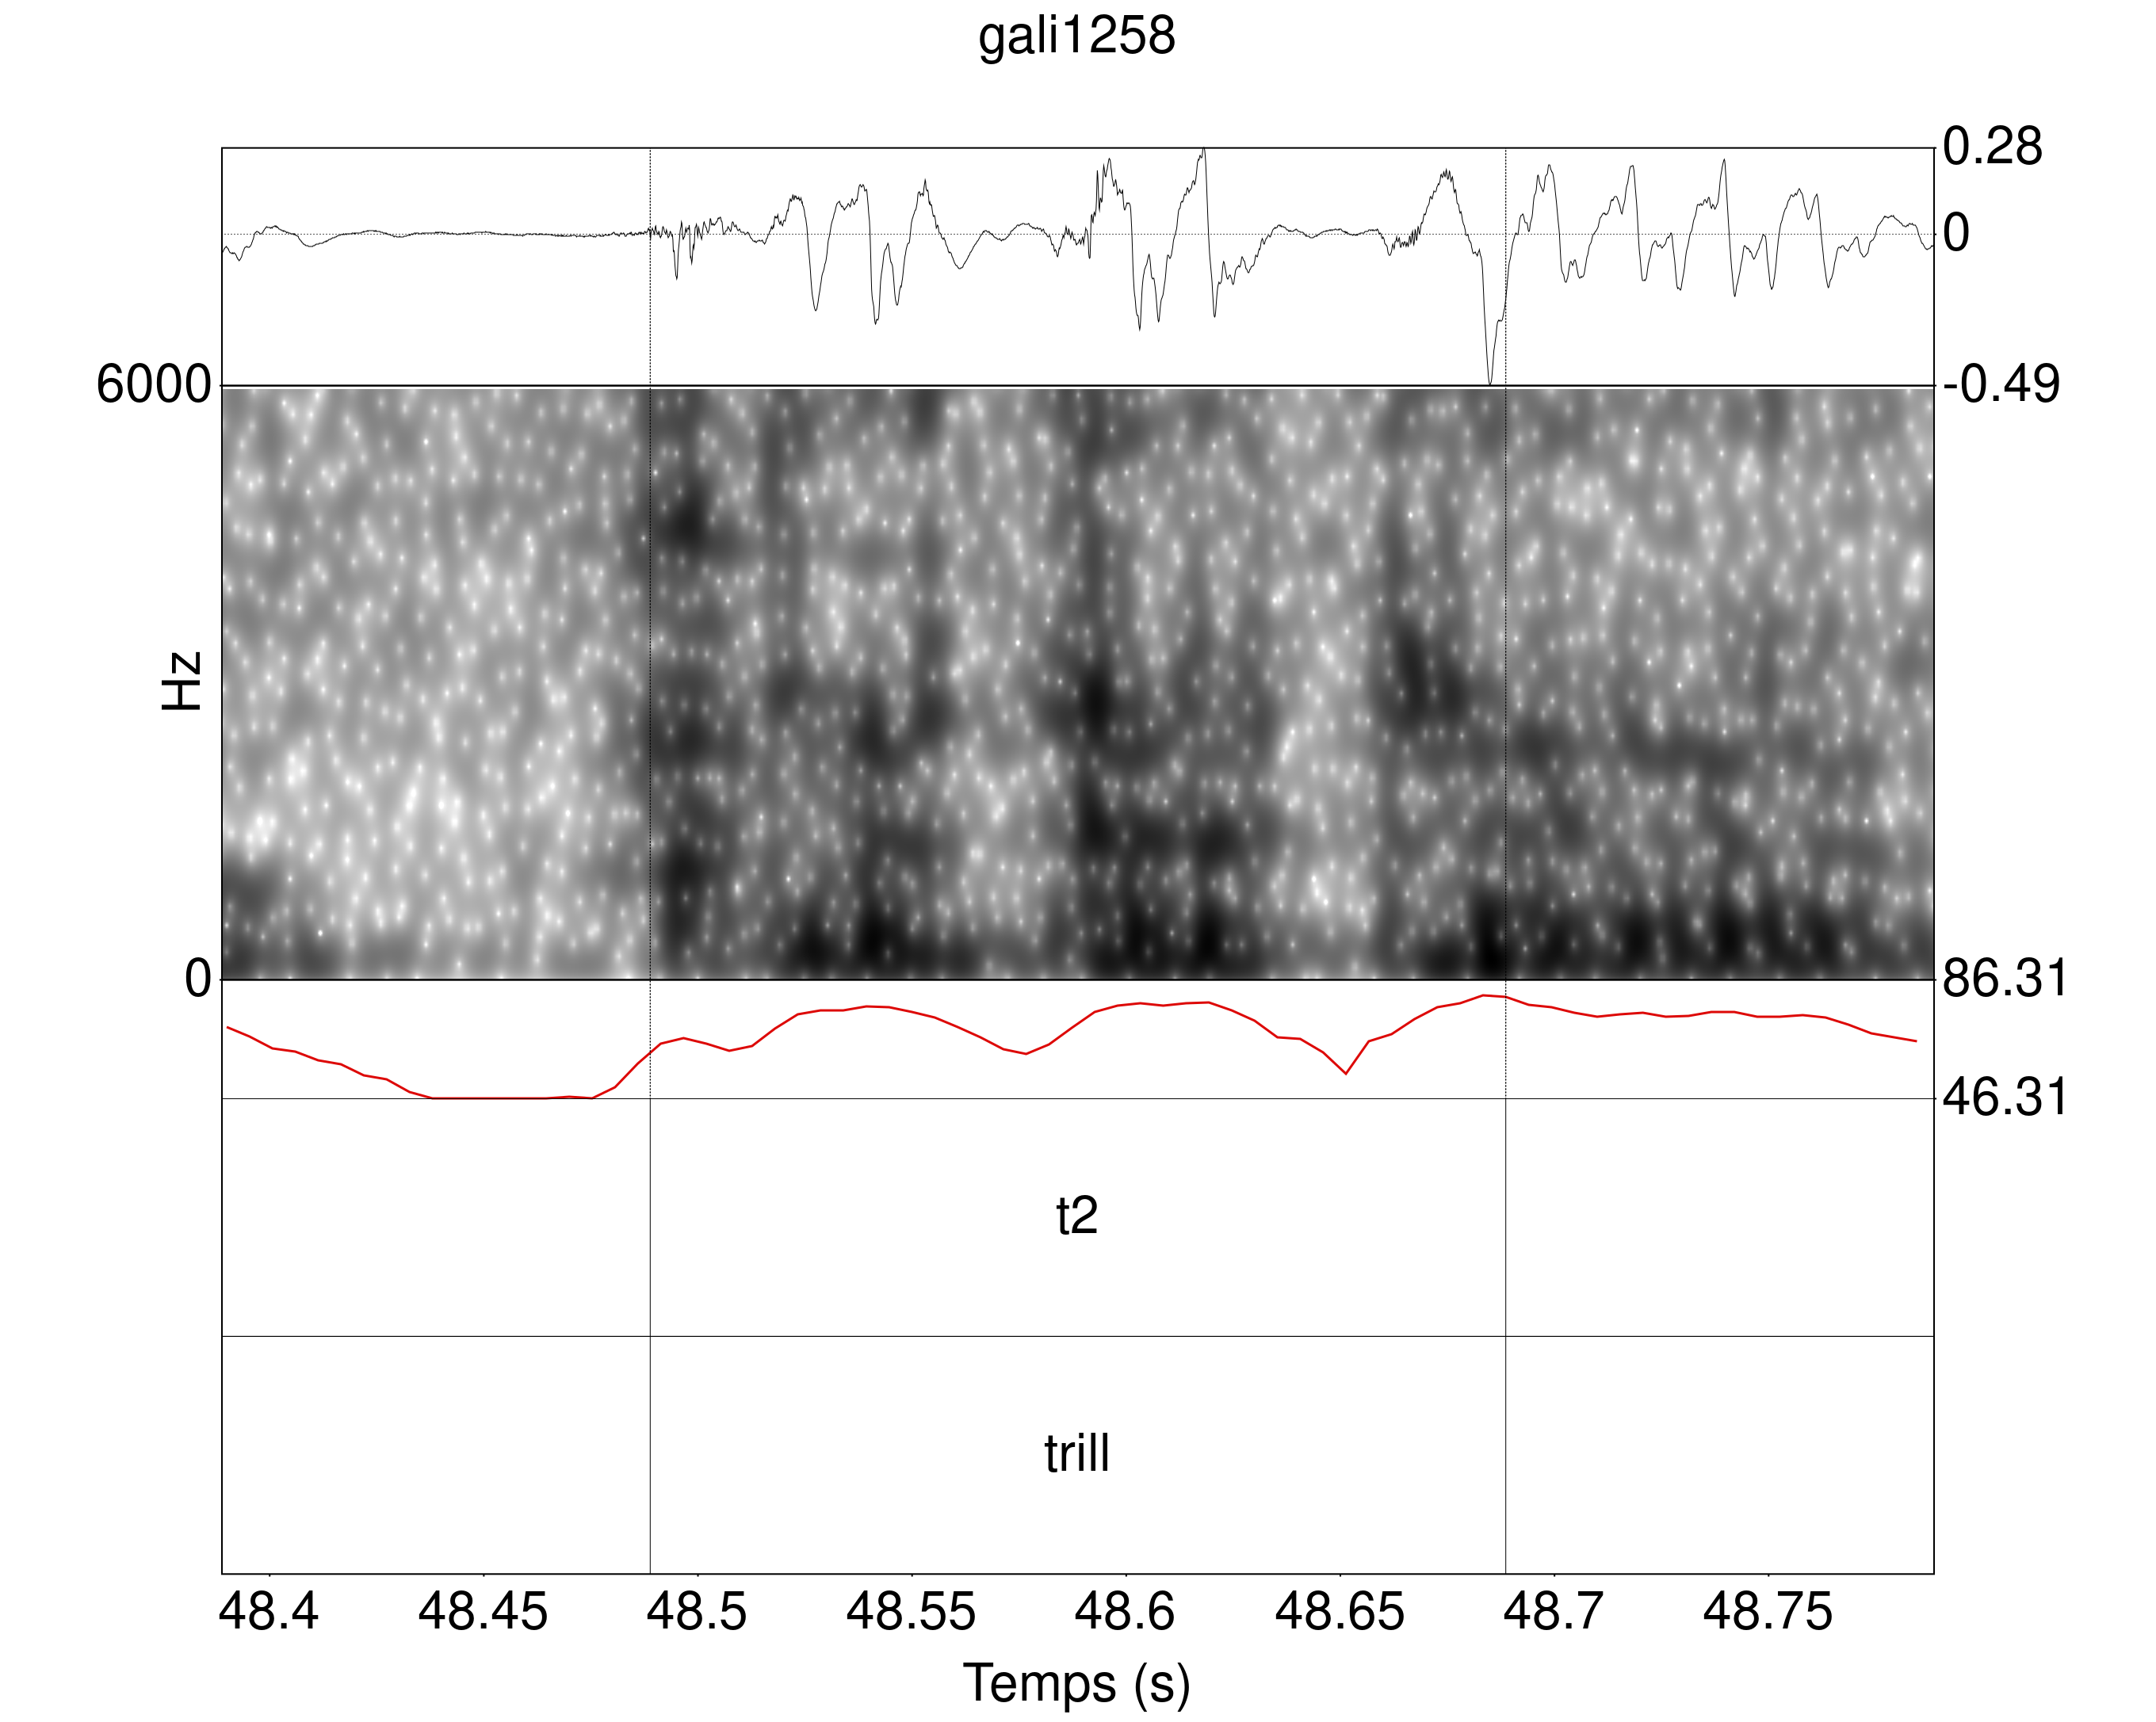
\includegraphics[width=0.45\linewidth]{substance/spectro_images/gali1258_718_48}
	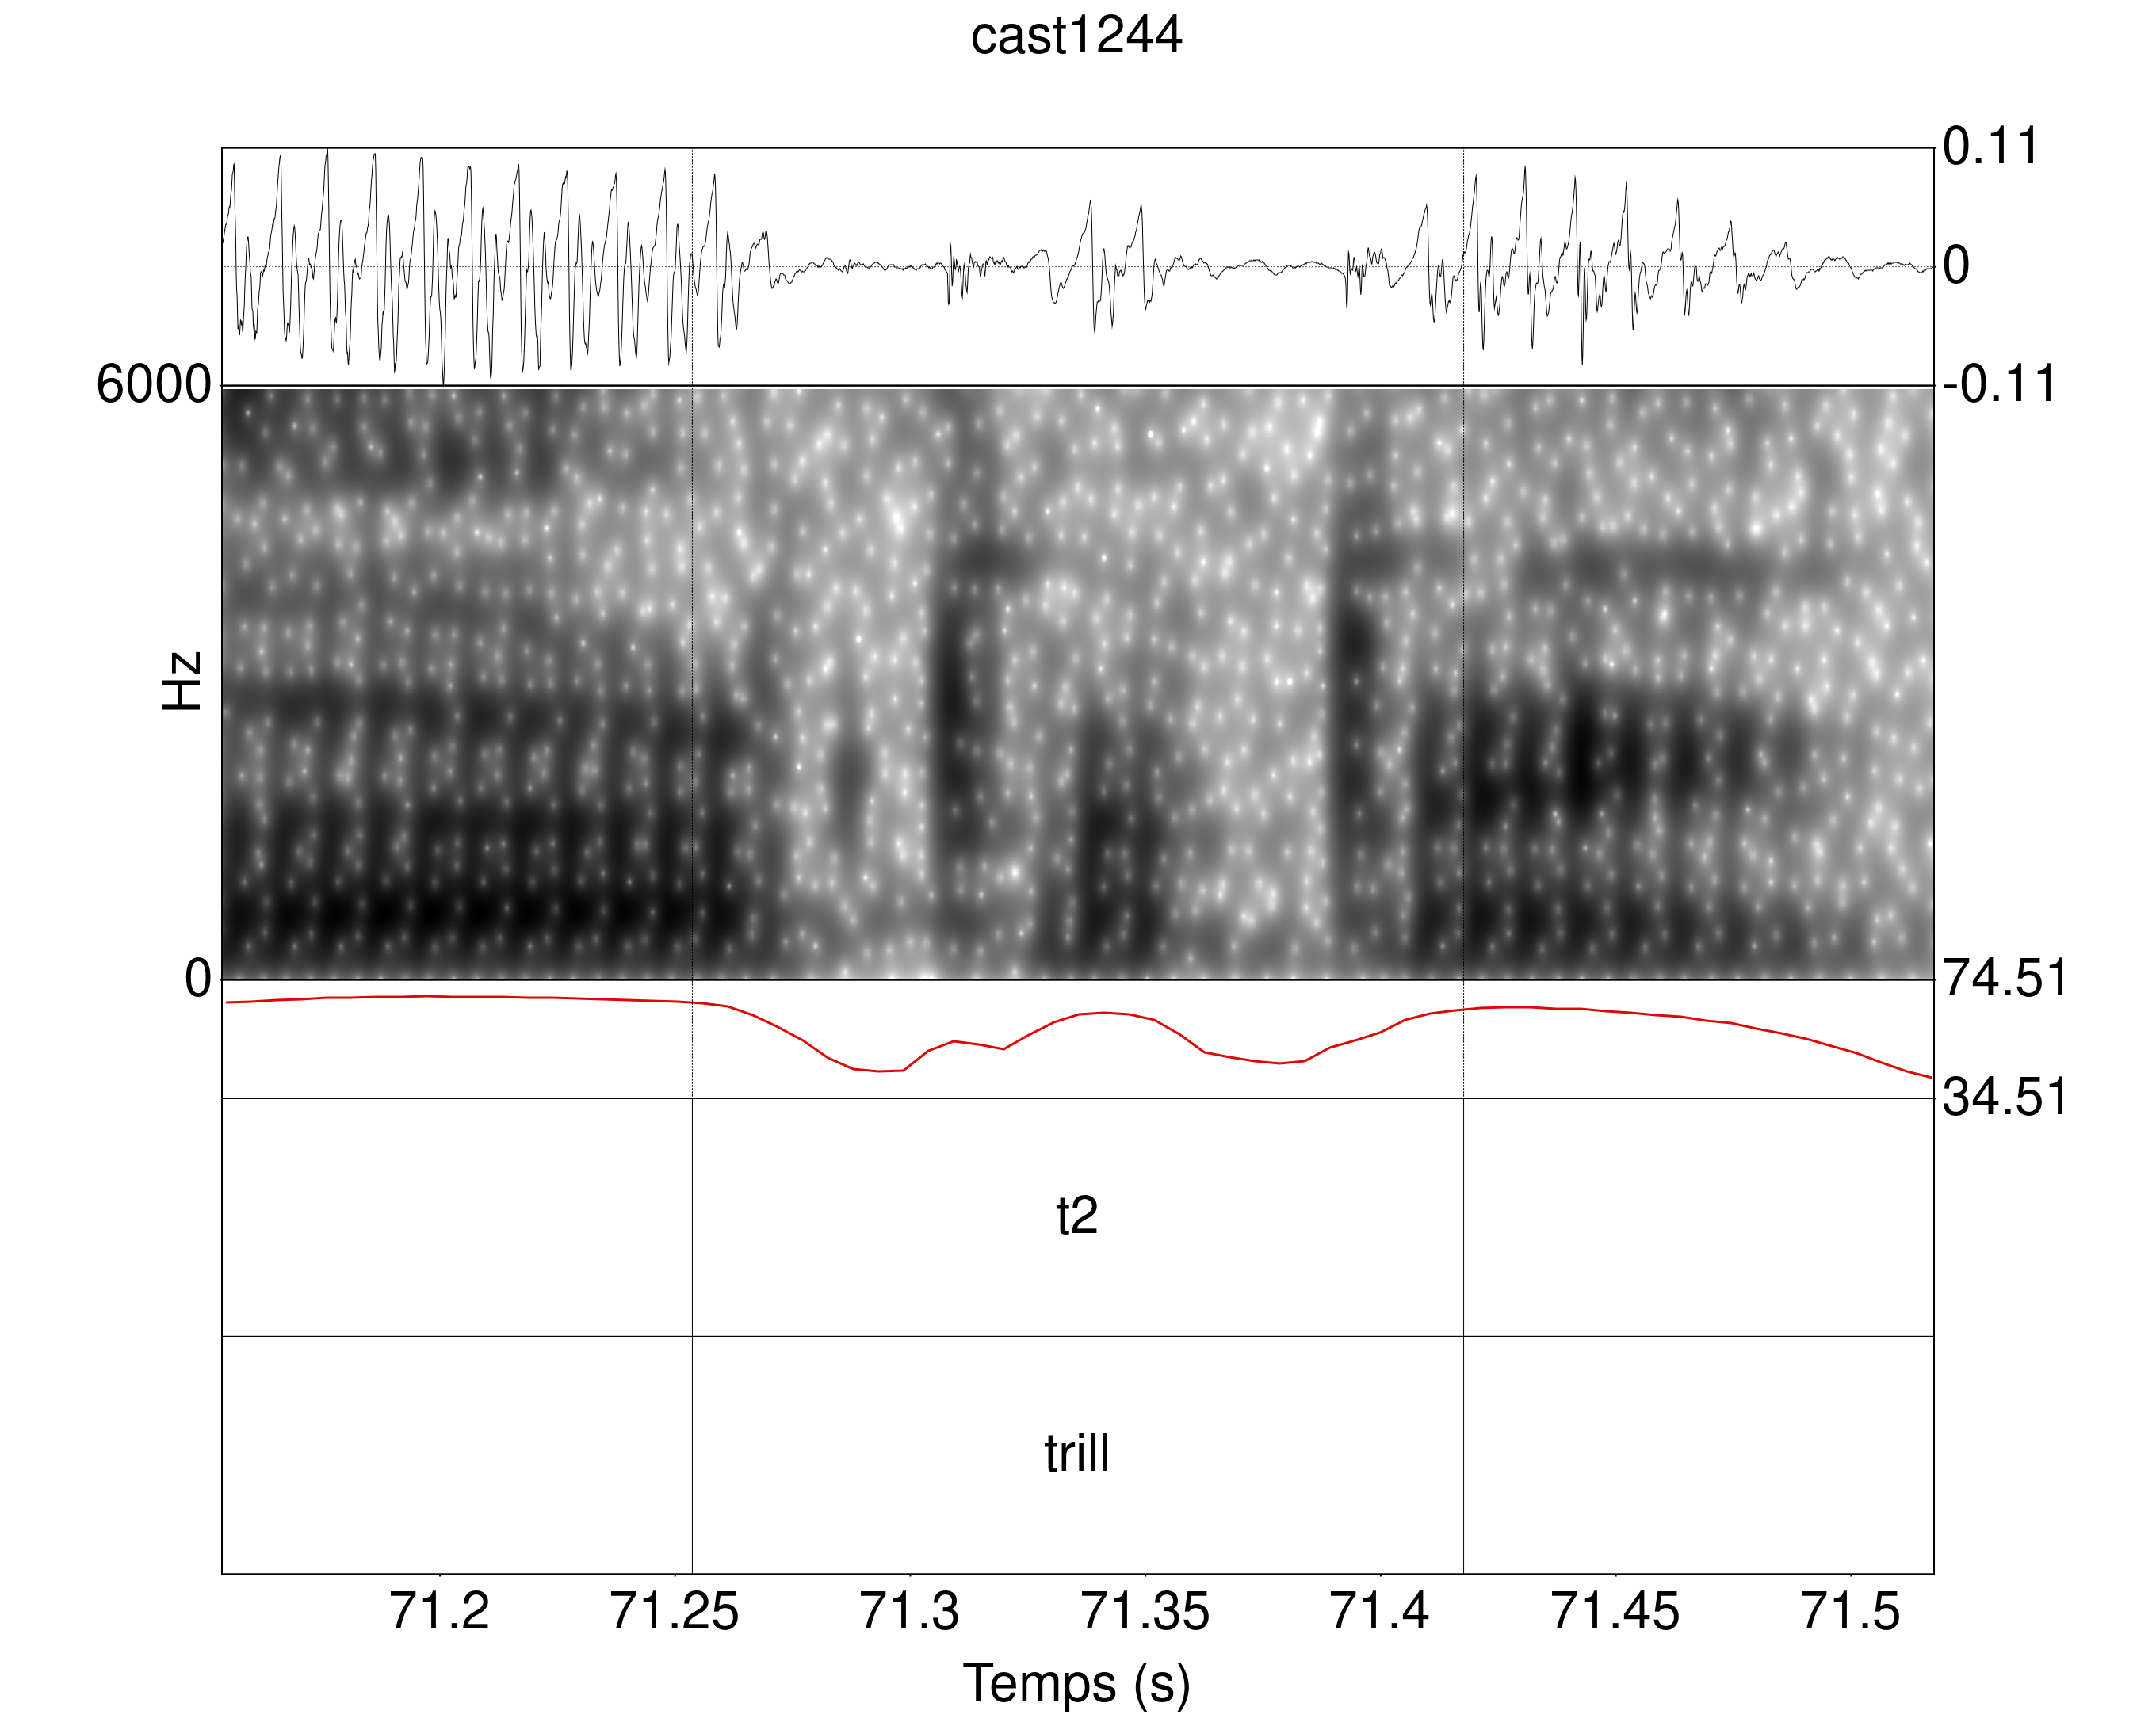
\includegraphics[width=0.45\linewidth]{substance/spectro_images/cast1244_354_66}
	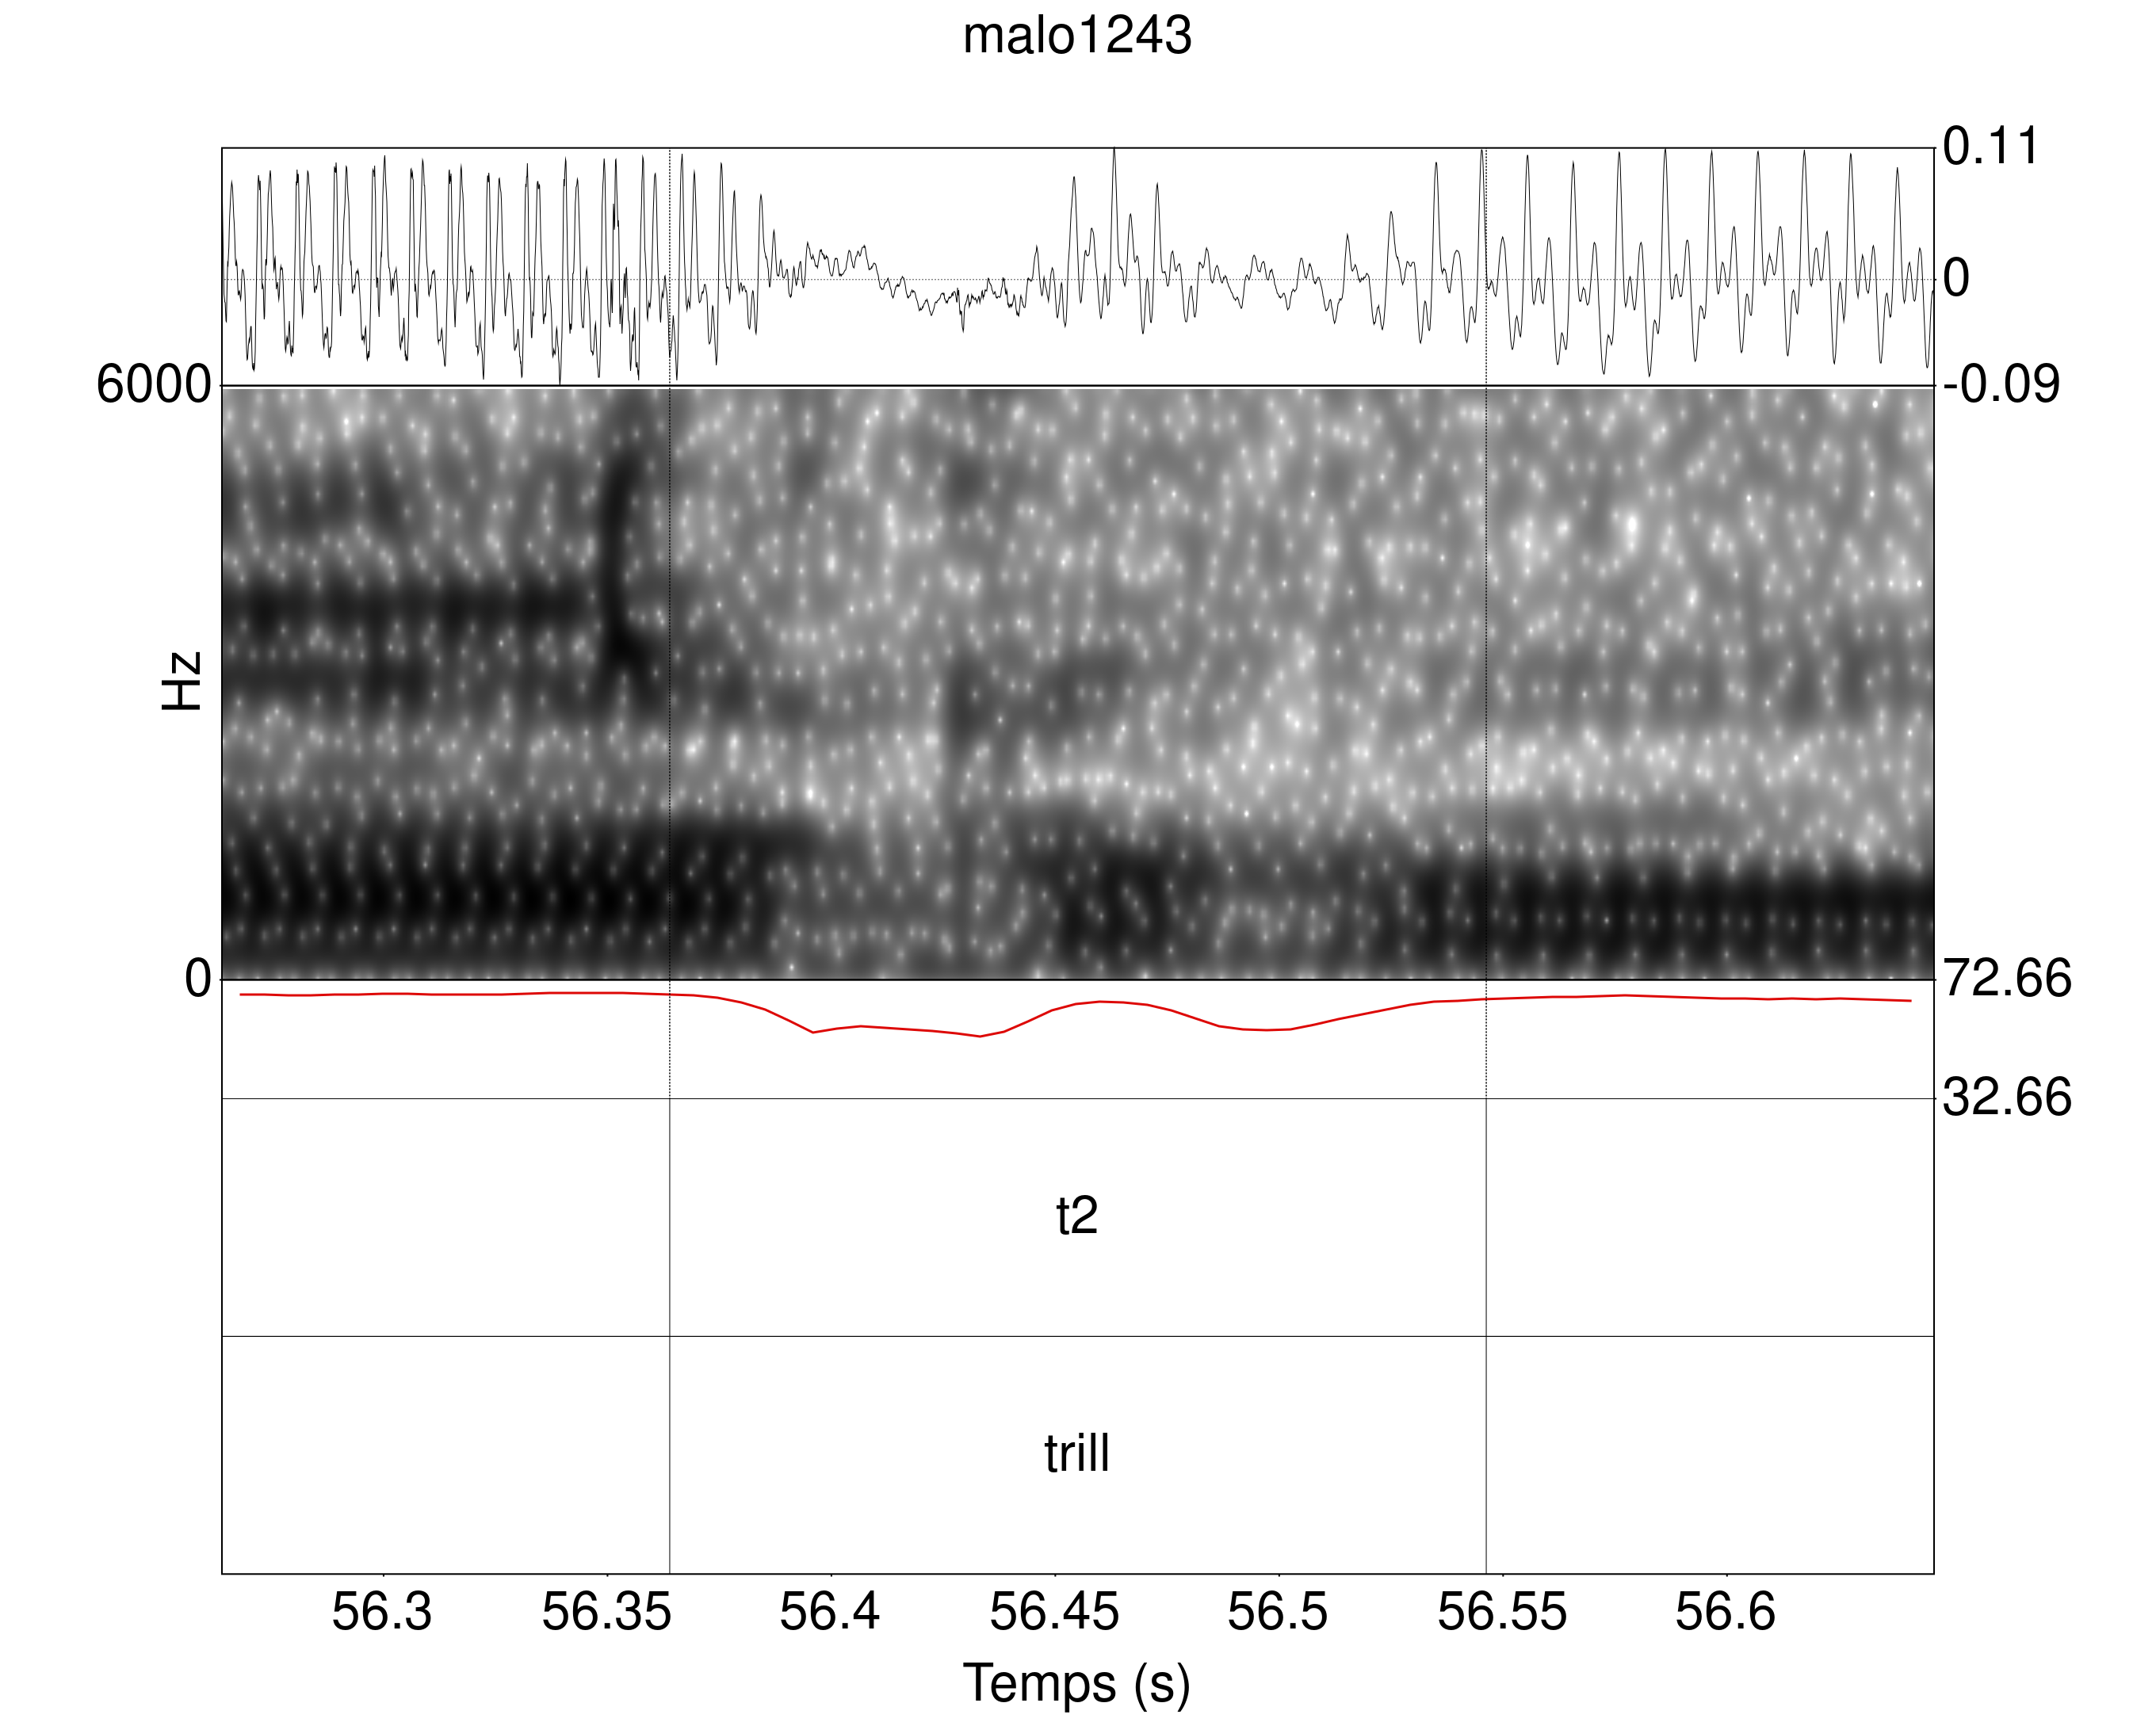
\includegraphics[width=0.45\linewidth]{substance/spectro_images/malo1243_1132_28}
	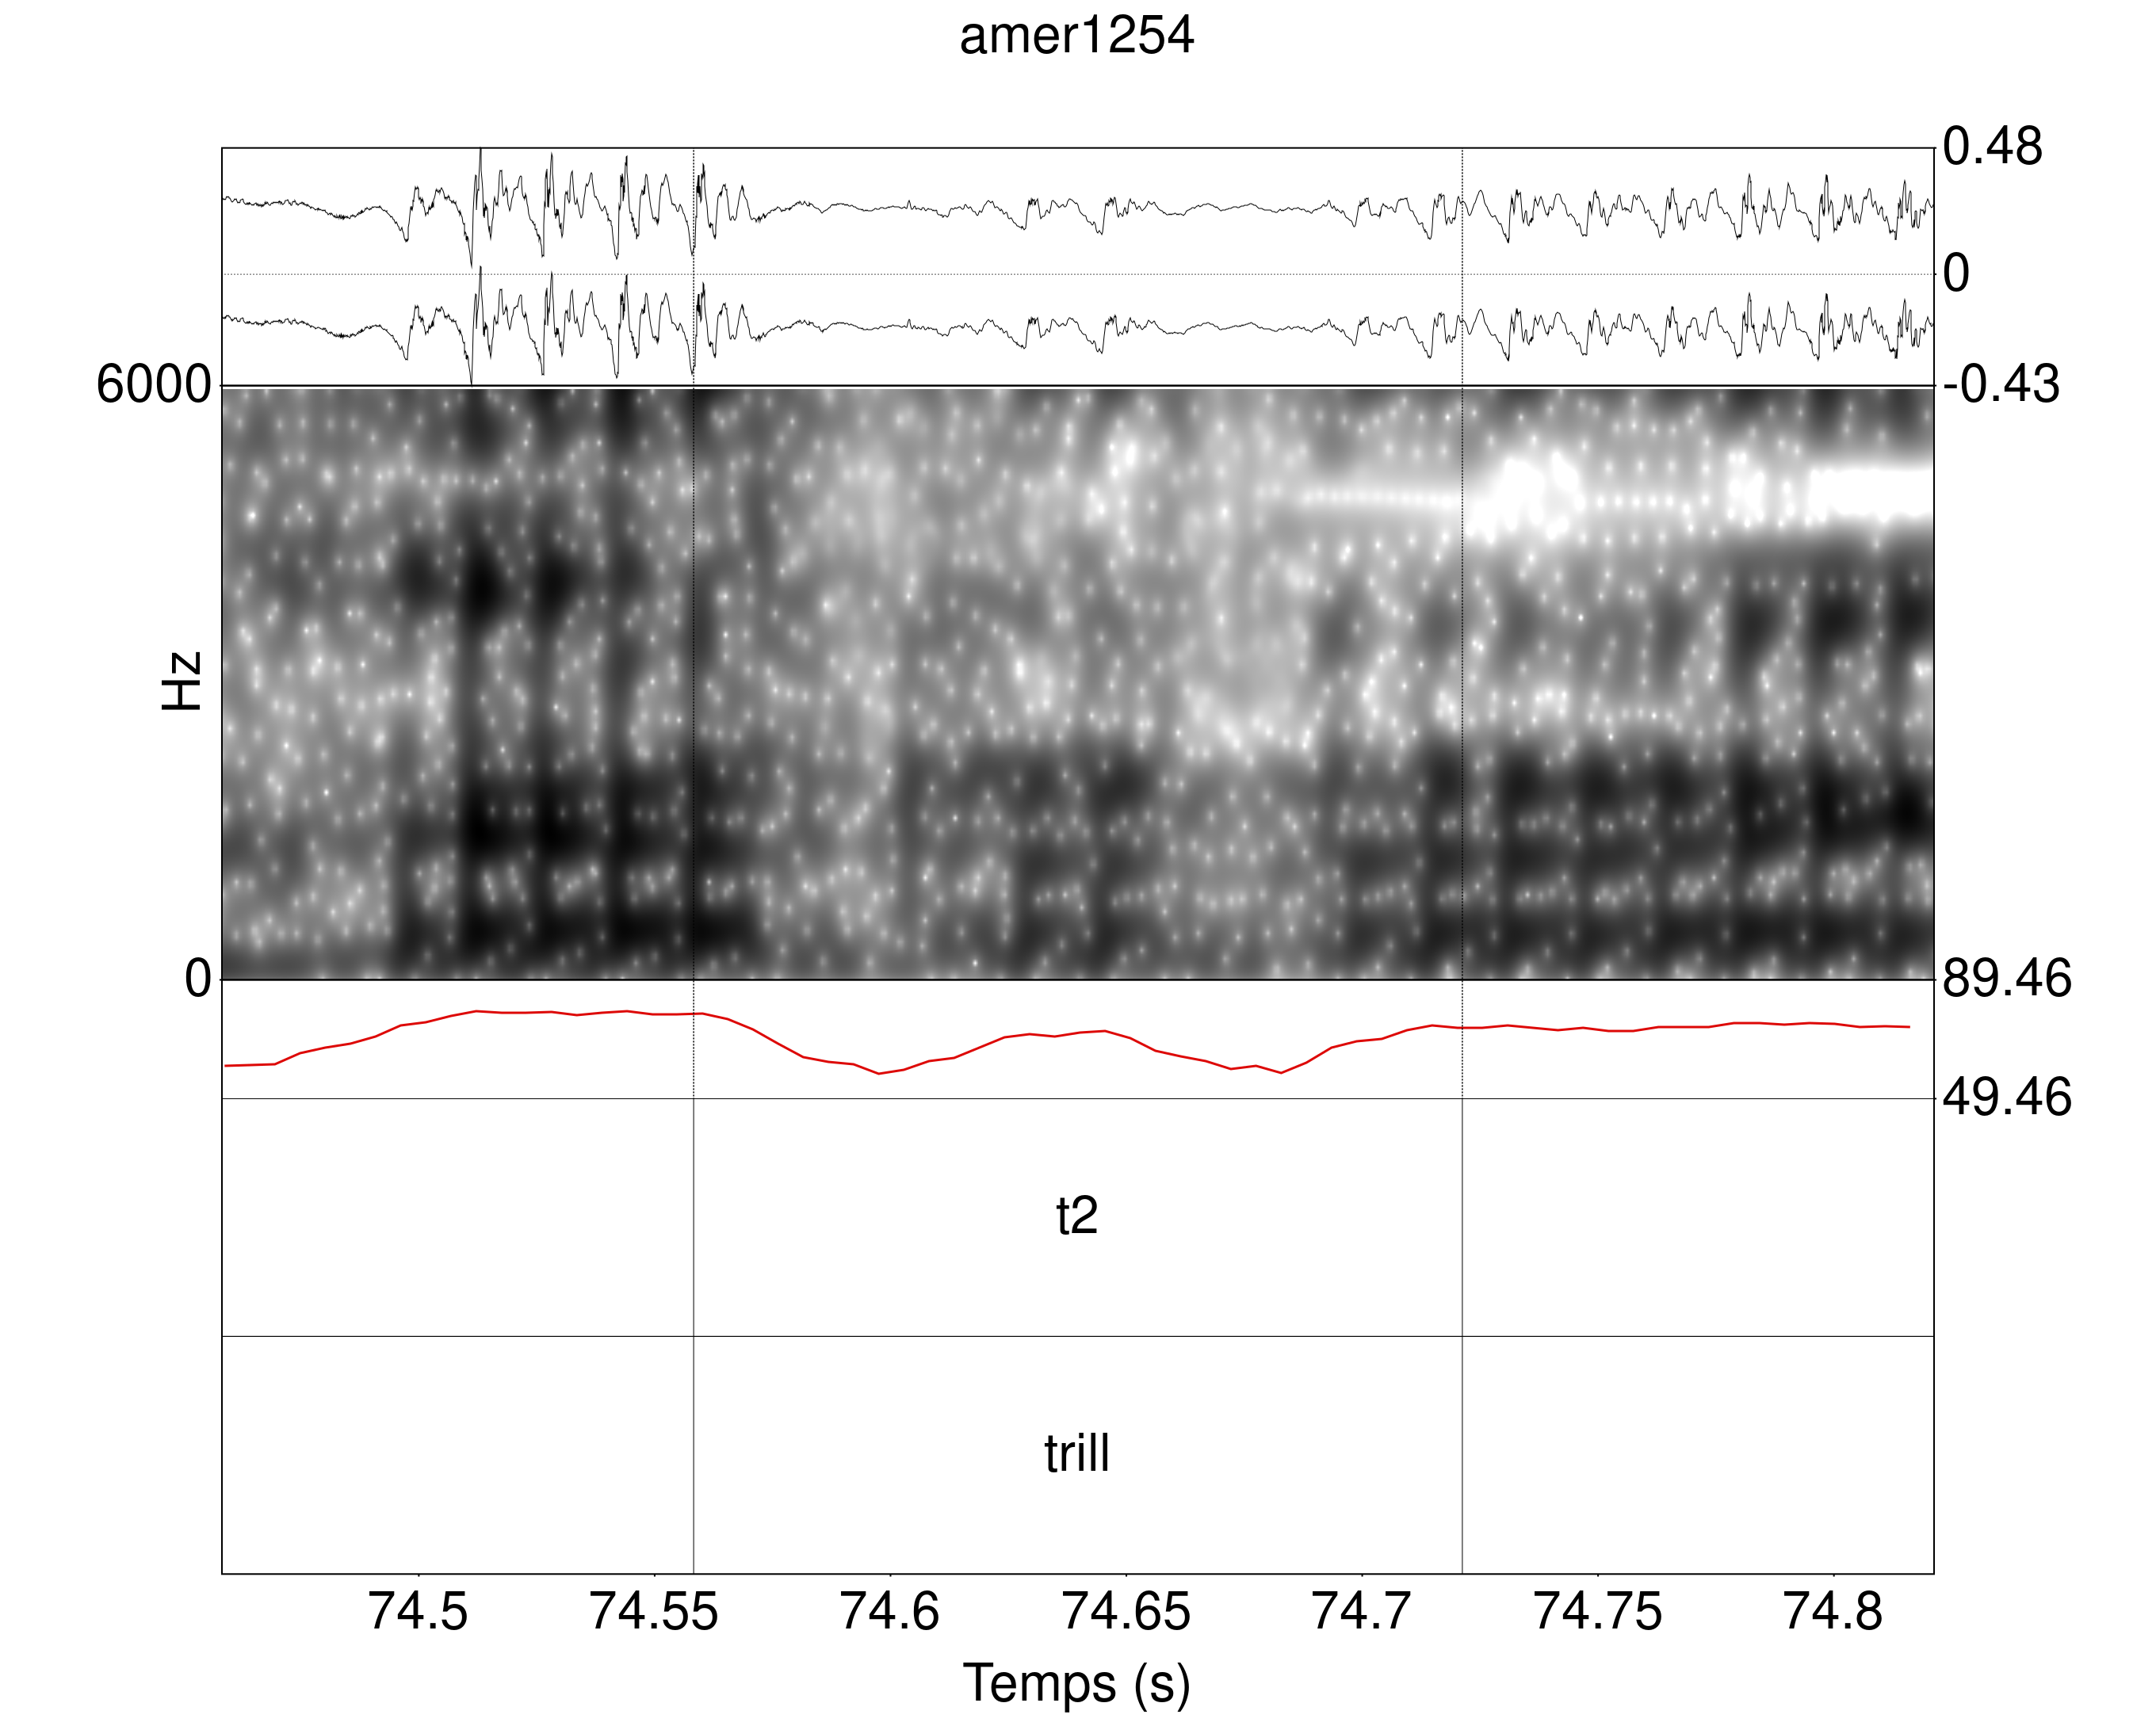
\includegraphics[width=0.45\linewidth]{substance/spectro_images/amer1254_67_62}
	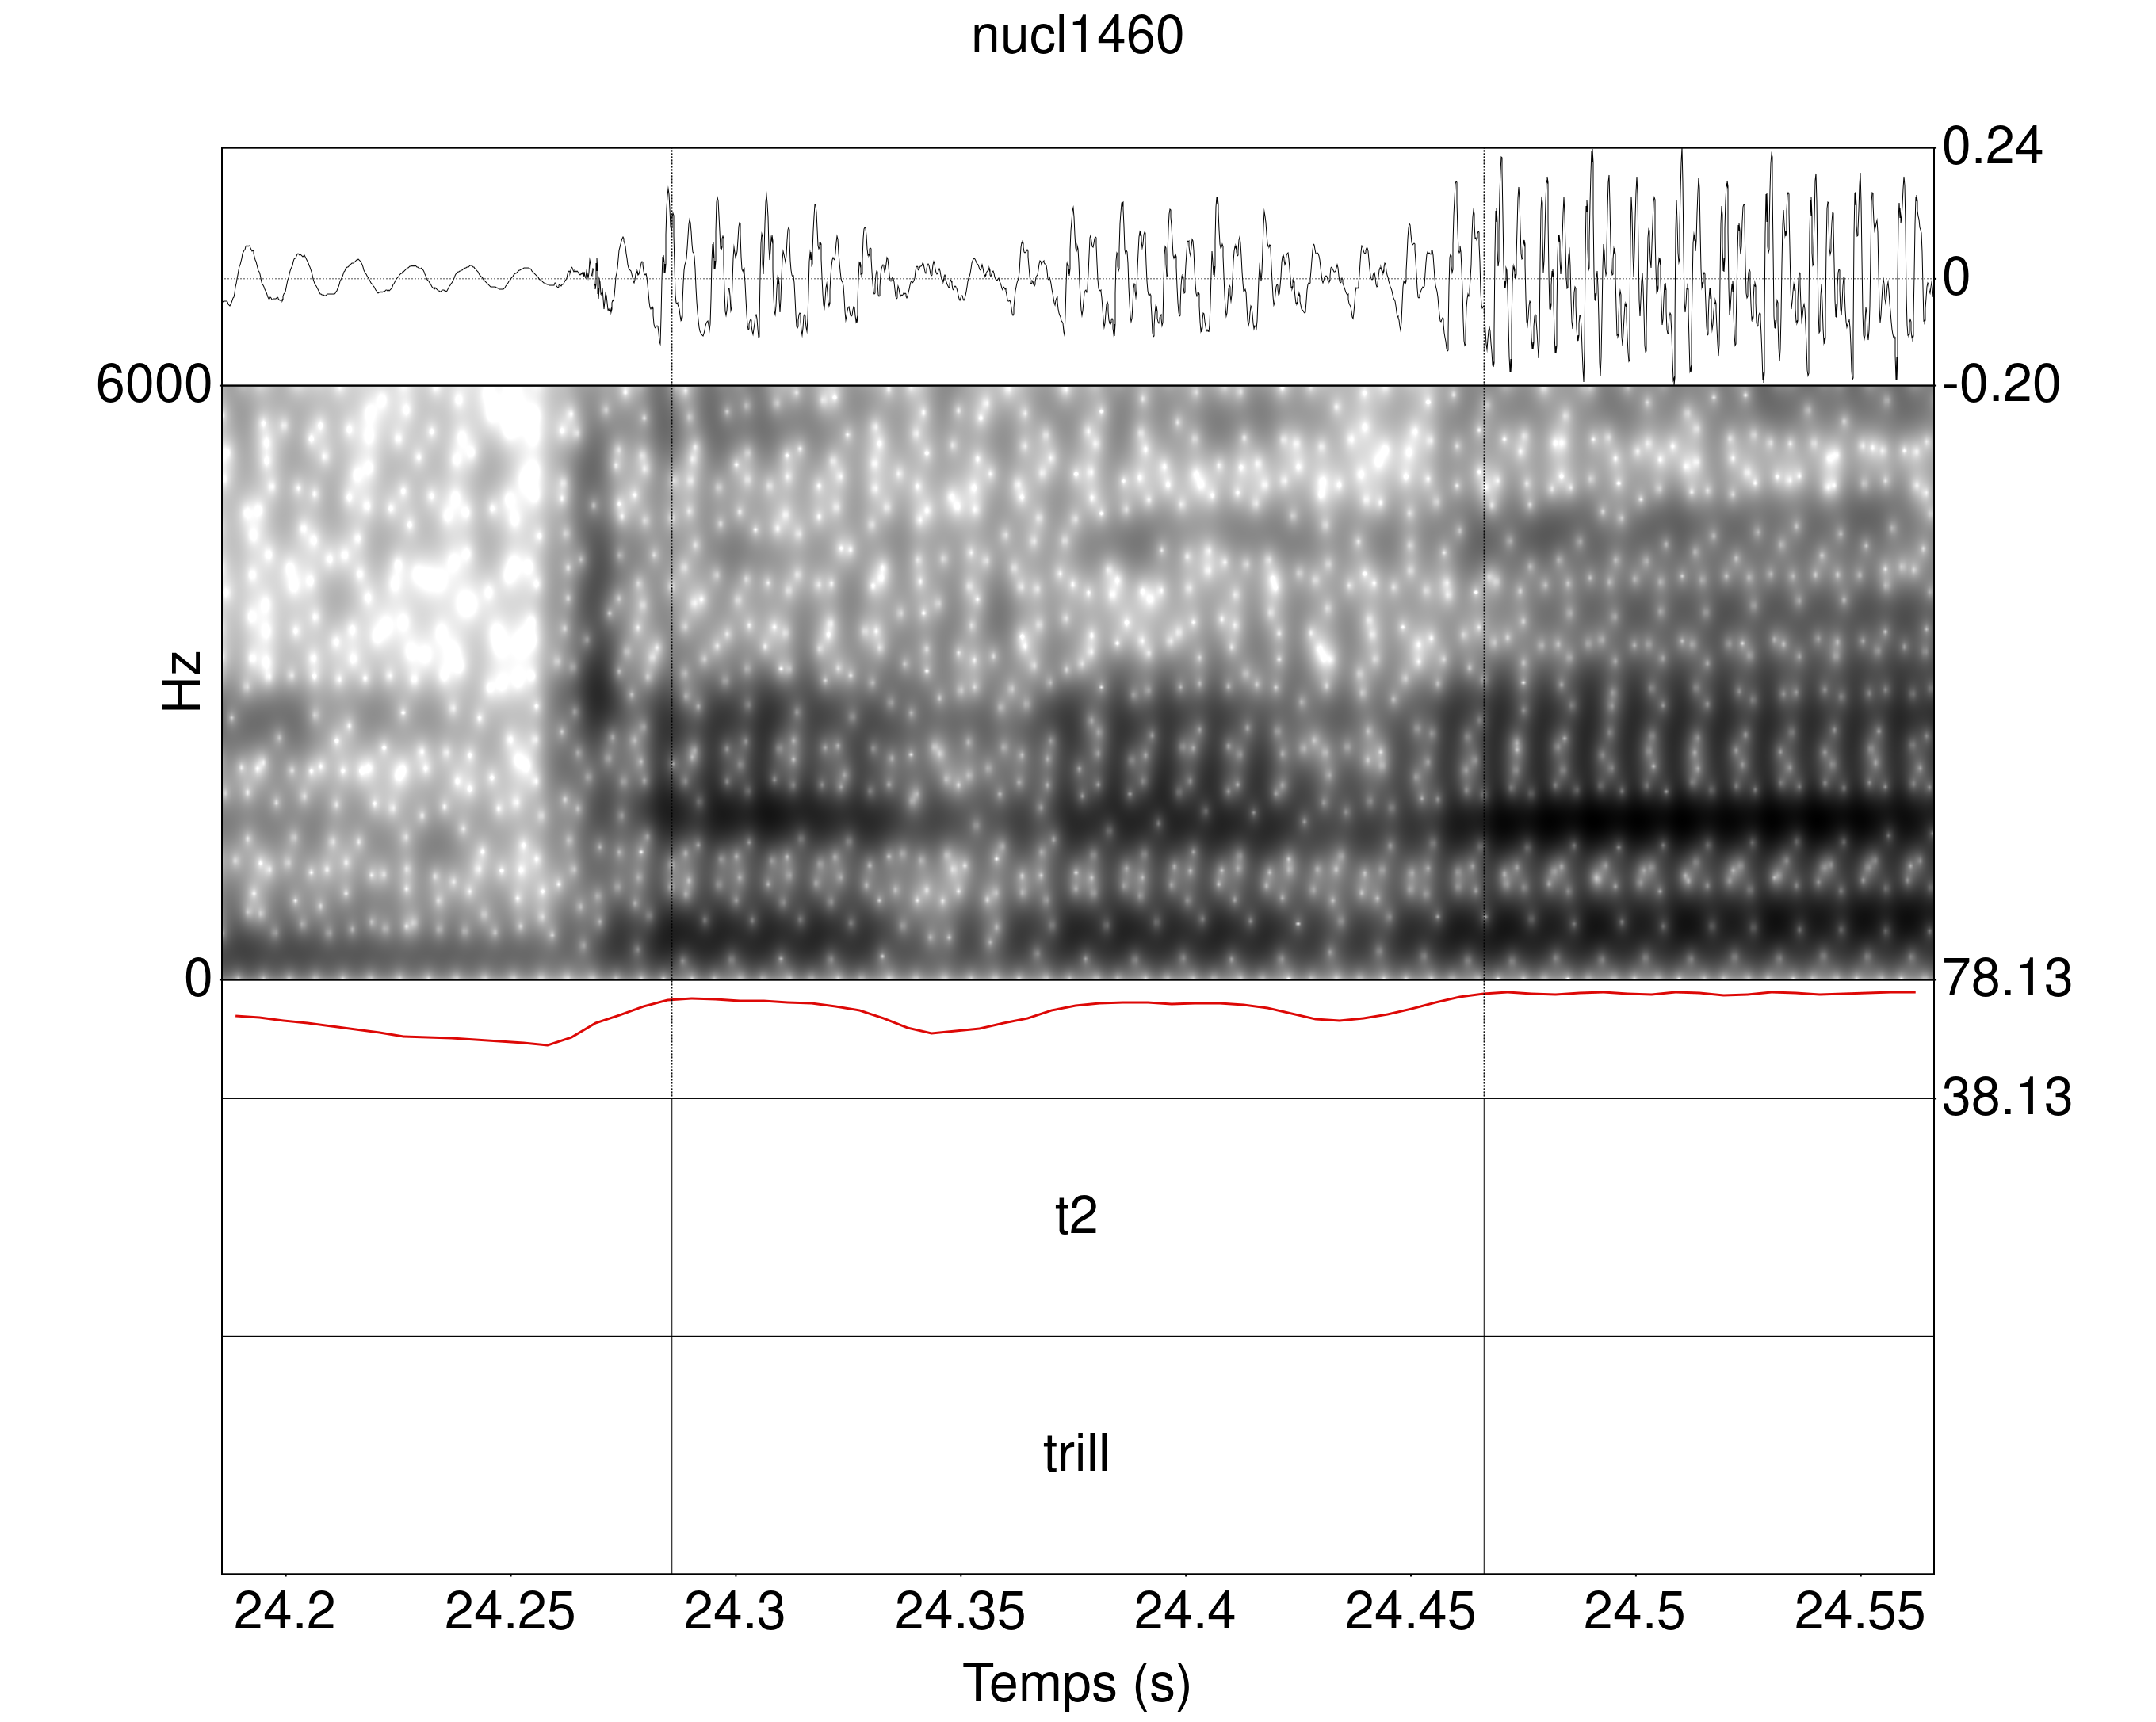
\includegraphics[width=0.45\linewidth]{substance/spectro_images/nucl1460_1338_16}
	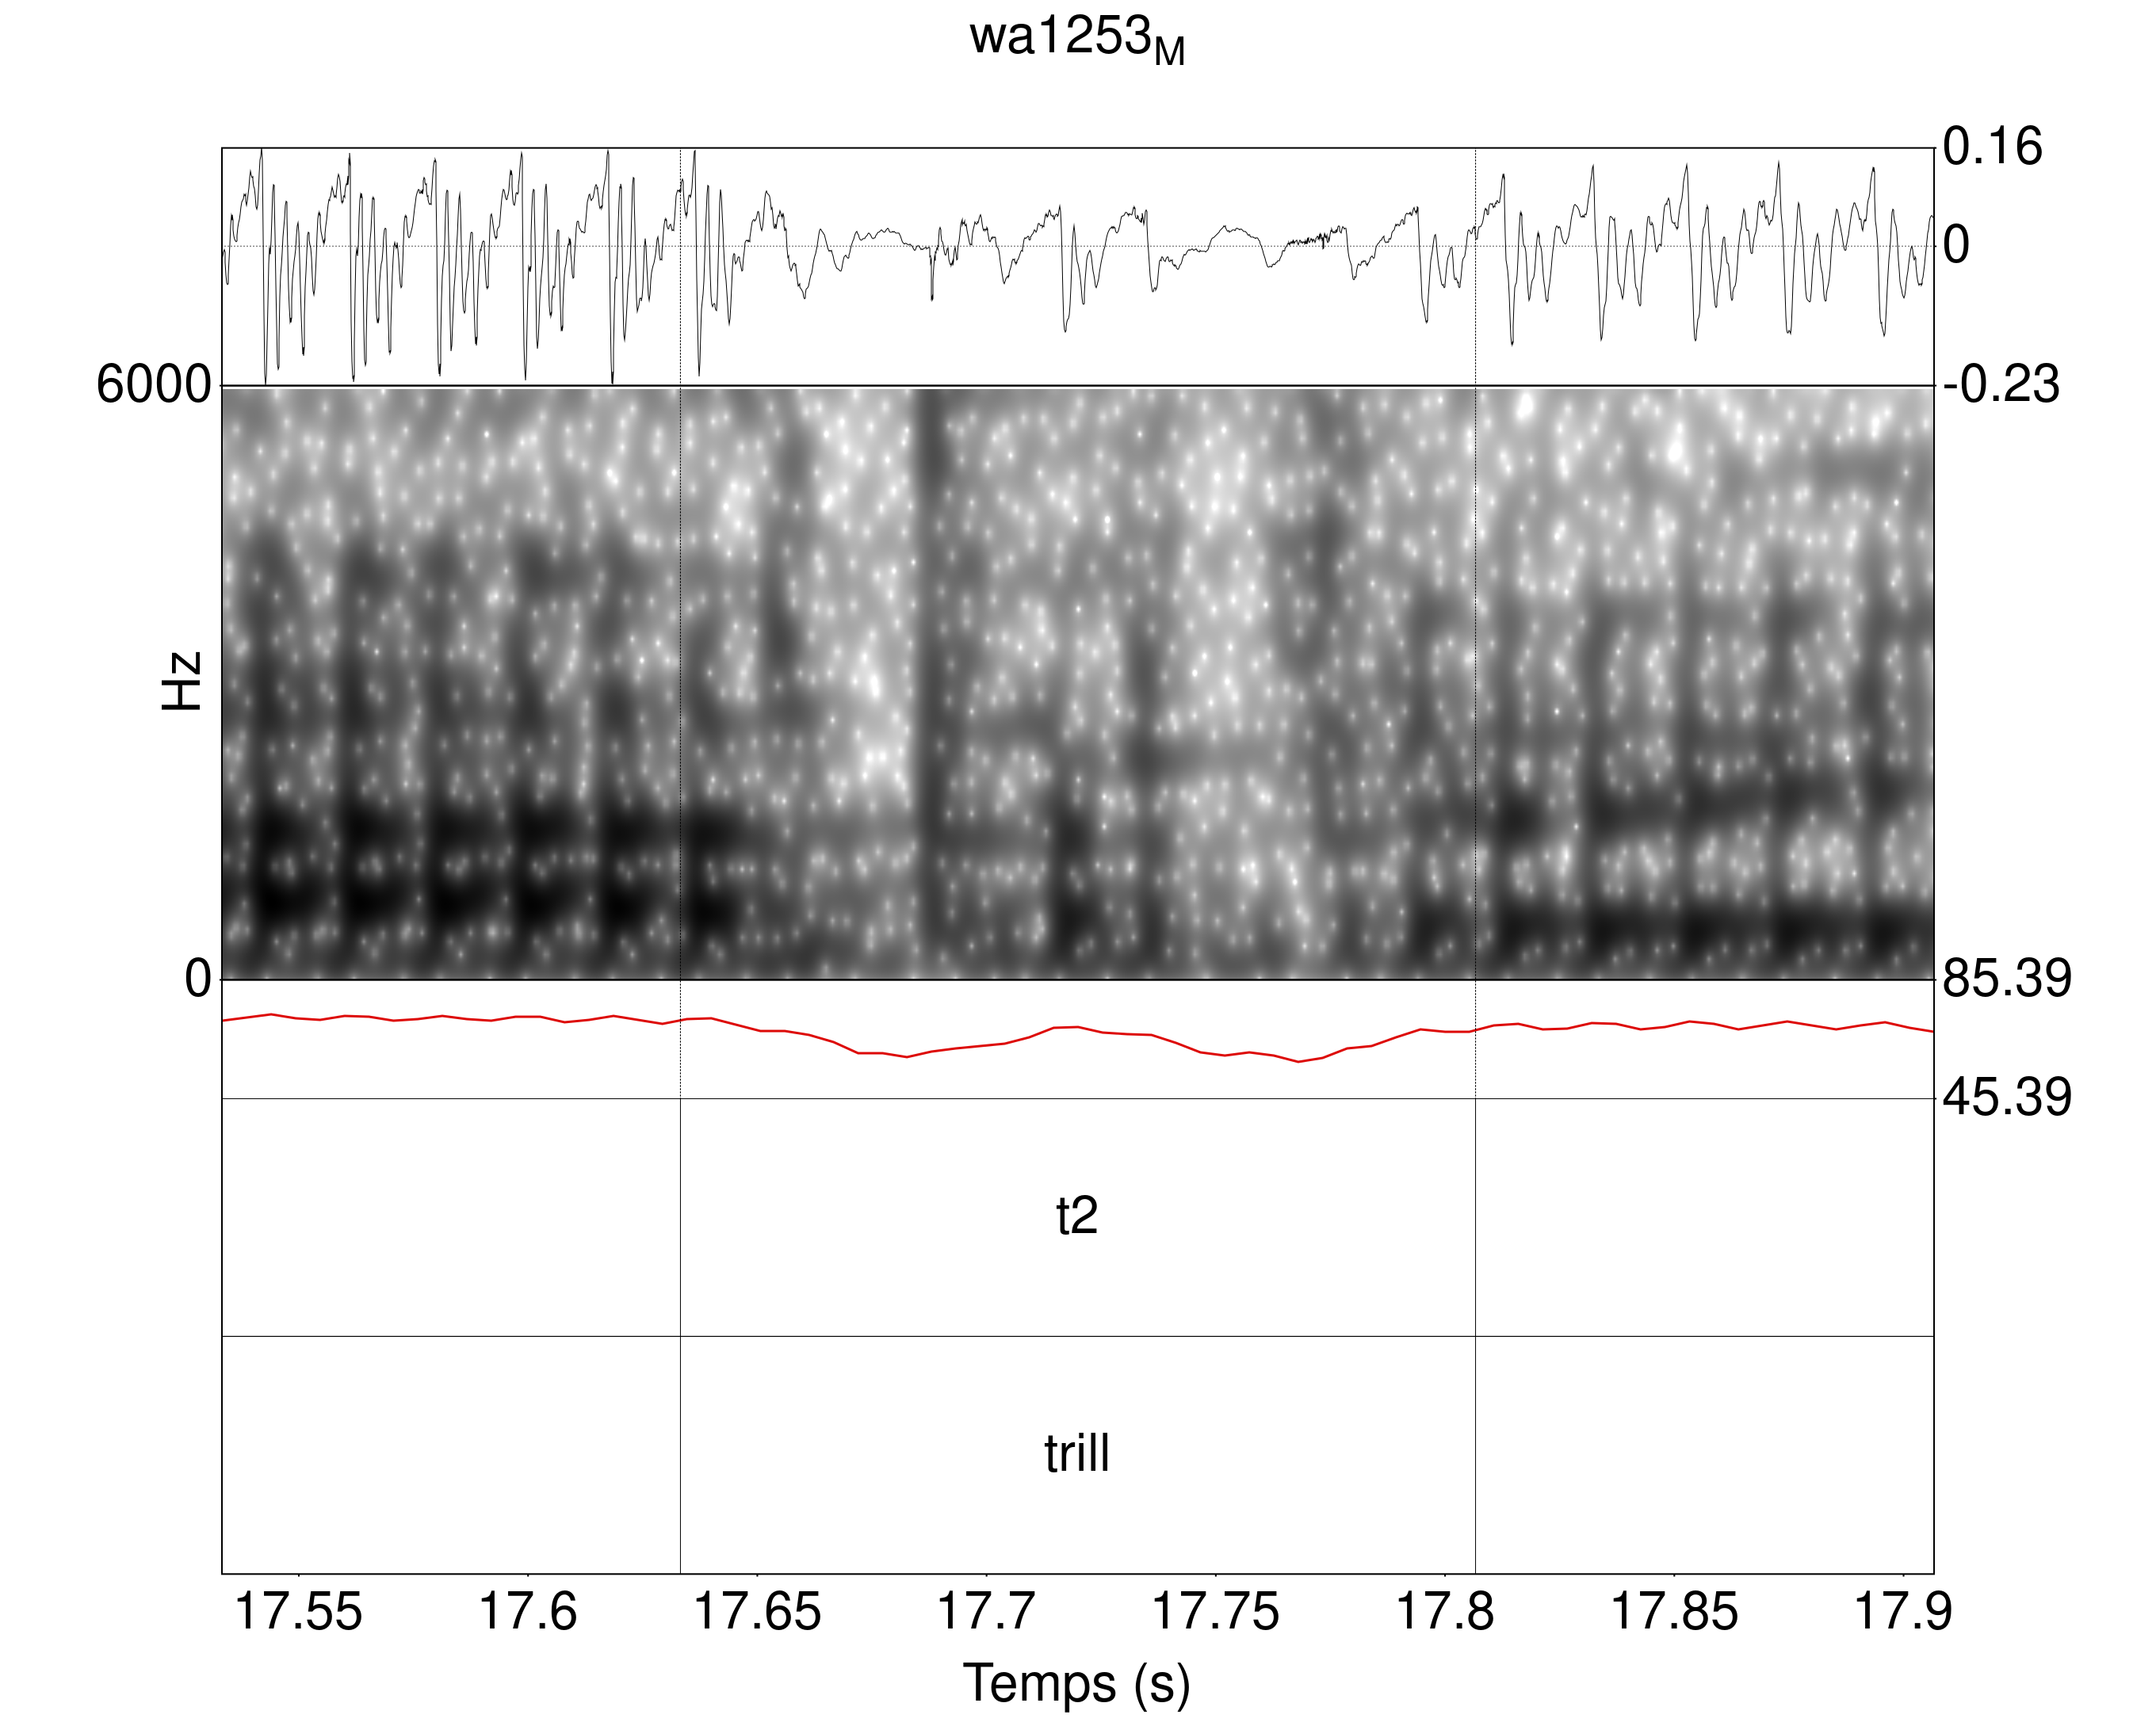
\includegraphics[width=0.45\linewidth]{substance/spectro_images/tswa1253_1703_6}
	\caption[Illustrations des \textg{t2} issus de 6 locuteurs et locutrices]{Illustrations avec oscillogrammes et spectrogrammes des \textg{t2} issus de locuteurs et locutrices
			du galicien \glotto{gali1258} (1 occurrence sur 1 de t2 soit 100\% des trills),
		    de l'espagnol castillan \glotto{cast1244} (2 occurrences sur 2 de t2 soit 100\% des trills),
		     du tamambo \glotto{malo1243} (15 occurrences sur 19 de t2 soit 78,9\% des trills),
		     de l'espagnol argentin \glotto{amer1254} (2 occurrences sur 3 de t2 soit 66,7\% des trills),
		     du madurais \glotto{nucl1460} (6 occurrences sur 8 de t2 soit 75\% des trills),
		     et du tswana \glotto{tswa1253} (3 occurrences sur 7 de t2 soit 42,9\% des trills).}
	\label{fig:galicastmalotswa}
\end{figure}

Dans un deuxième temps, nous nous intéressons aux segments labellisés comme taps, flaps et taps/flaps.
Sur les 27 locuteurs/trices qui produisent ces segments (\autoref{fig:variationtapflap}), cinq ont produit au moins un \textg{t2} (voir \autoref{fig:pashsanm} pour les illustrations acoustiques de deux segments issus de ces cinq locuteurs/trices).

\begin{figure}
	\centering
	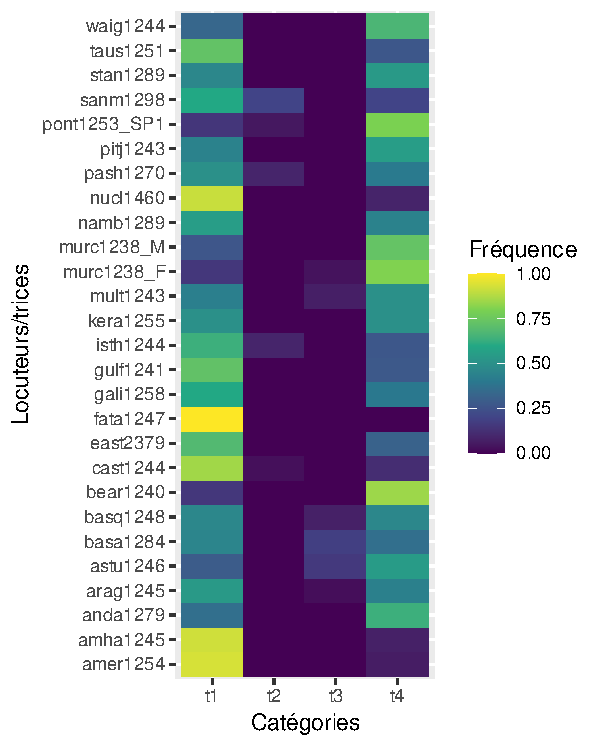
\includegraphics[width=0.45\linewidth]{substance/images/variation_tapflap}
	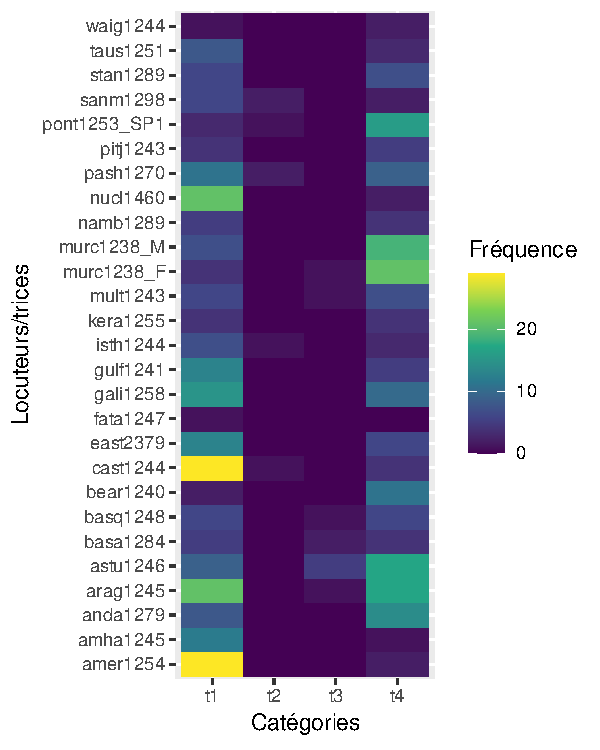
\includegraphics[width=0.45\linewidth]{substance/images/variation_tapflap_abs}
	\caption[Fréquences des différentes catégories illustrant la variation pour les segments ayant été catégorisés comme des \textg{taps, flaps et taps/flaps}]{Fréquences relatives (à gauche) et absolues (à droite) des différentes catégories illustrant la variation pour les segments ayant été catégorisés par les auteurs des illustrations comme des \textg{taps, flaps et taps/flaps}. Les fréquences sont calculées par ligne. Une case jaune est associée à une haute fréquence, cela veut dire que le/la locuteur/trice tend à produire une seule catégorie. Une case violette est associée à une catégorie non produite par le/la locuteur/trice.}
	\label{fig:variationtapflap}
\end{figure}

\begin{figure}
	\centering
	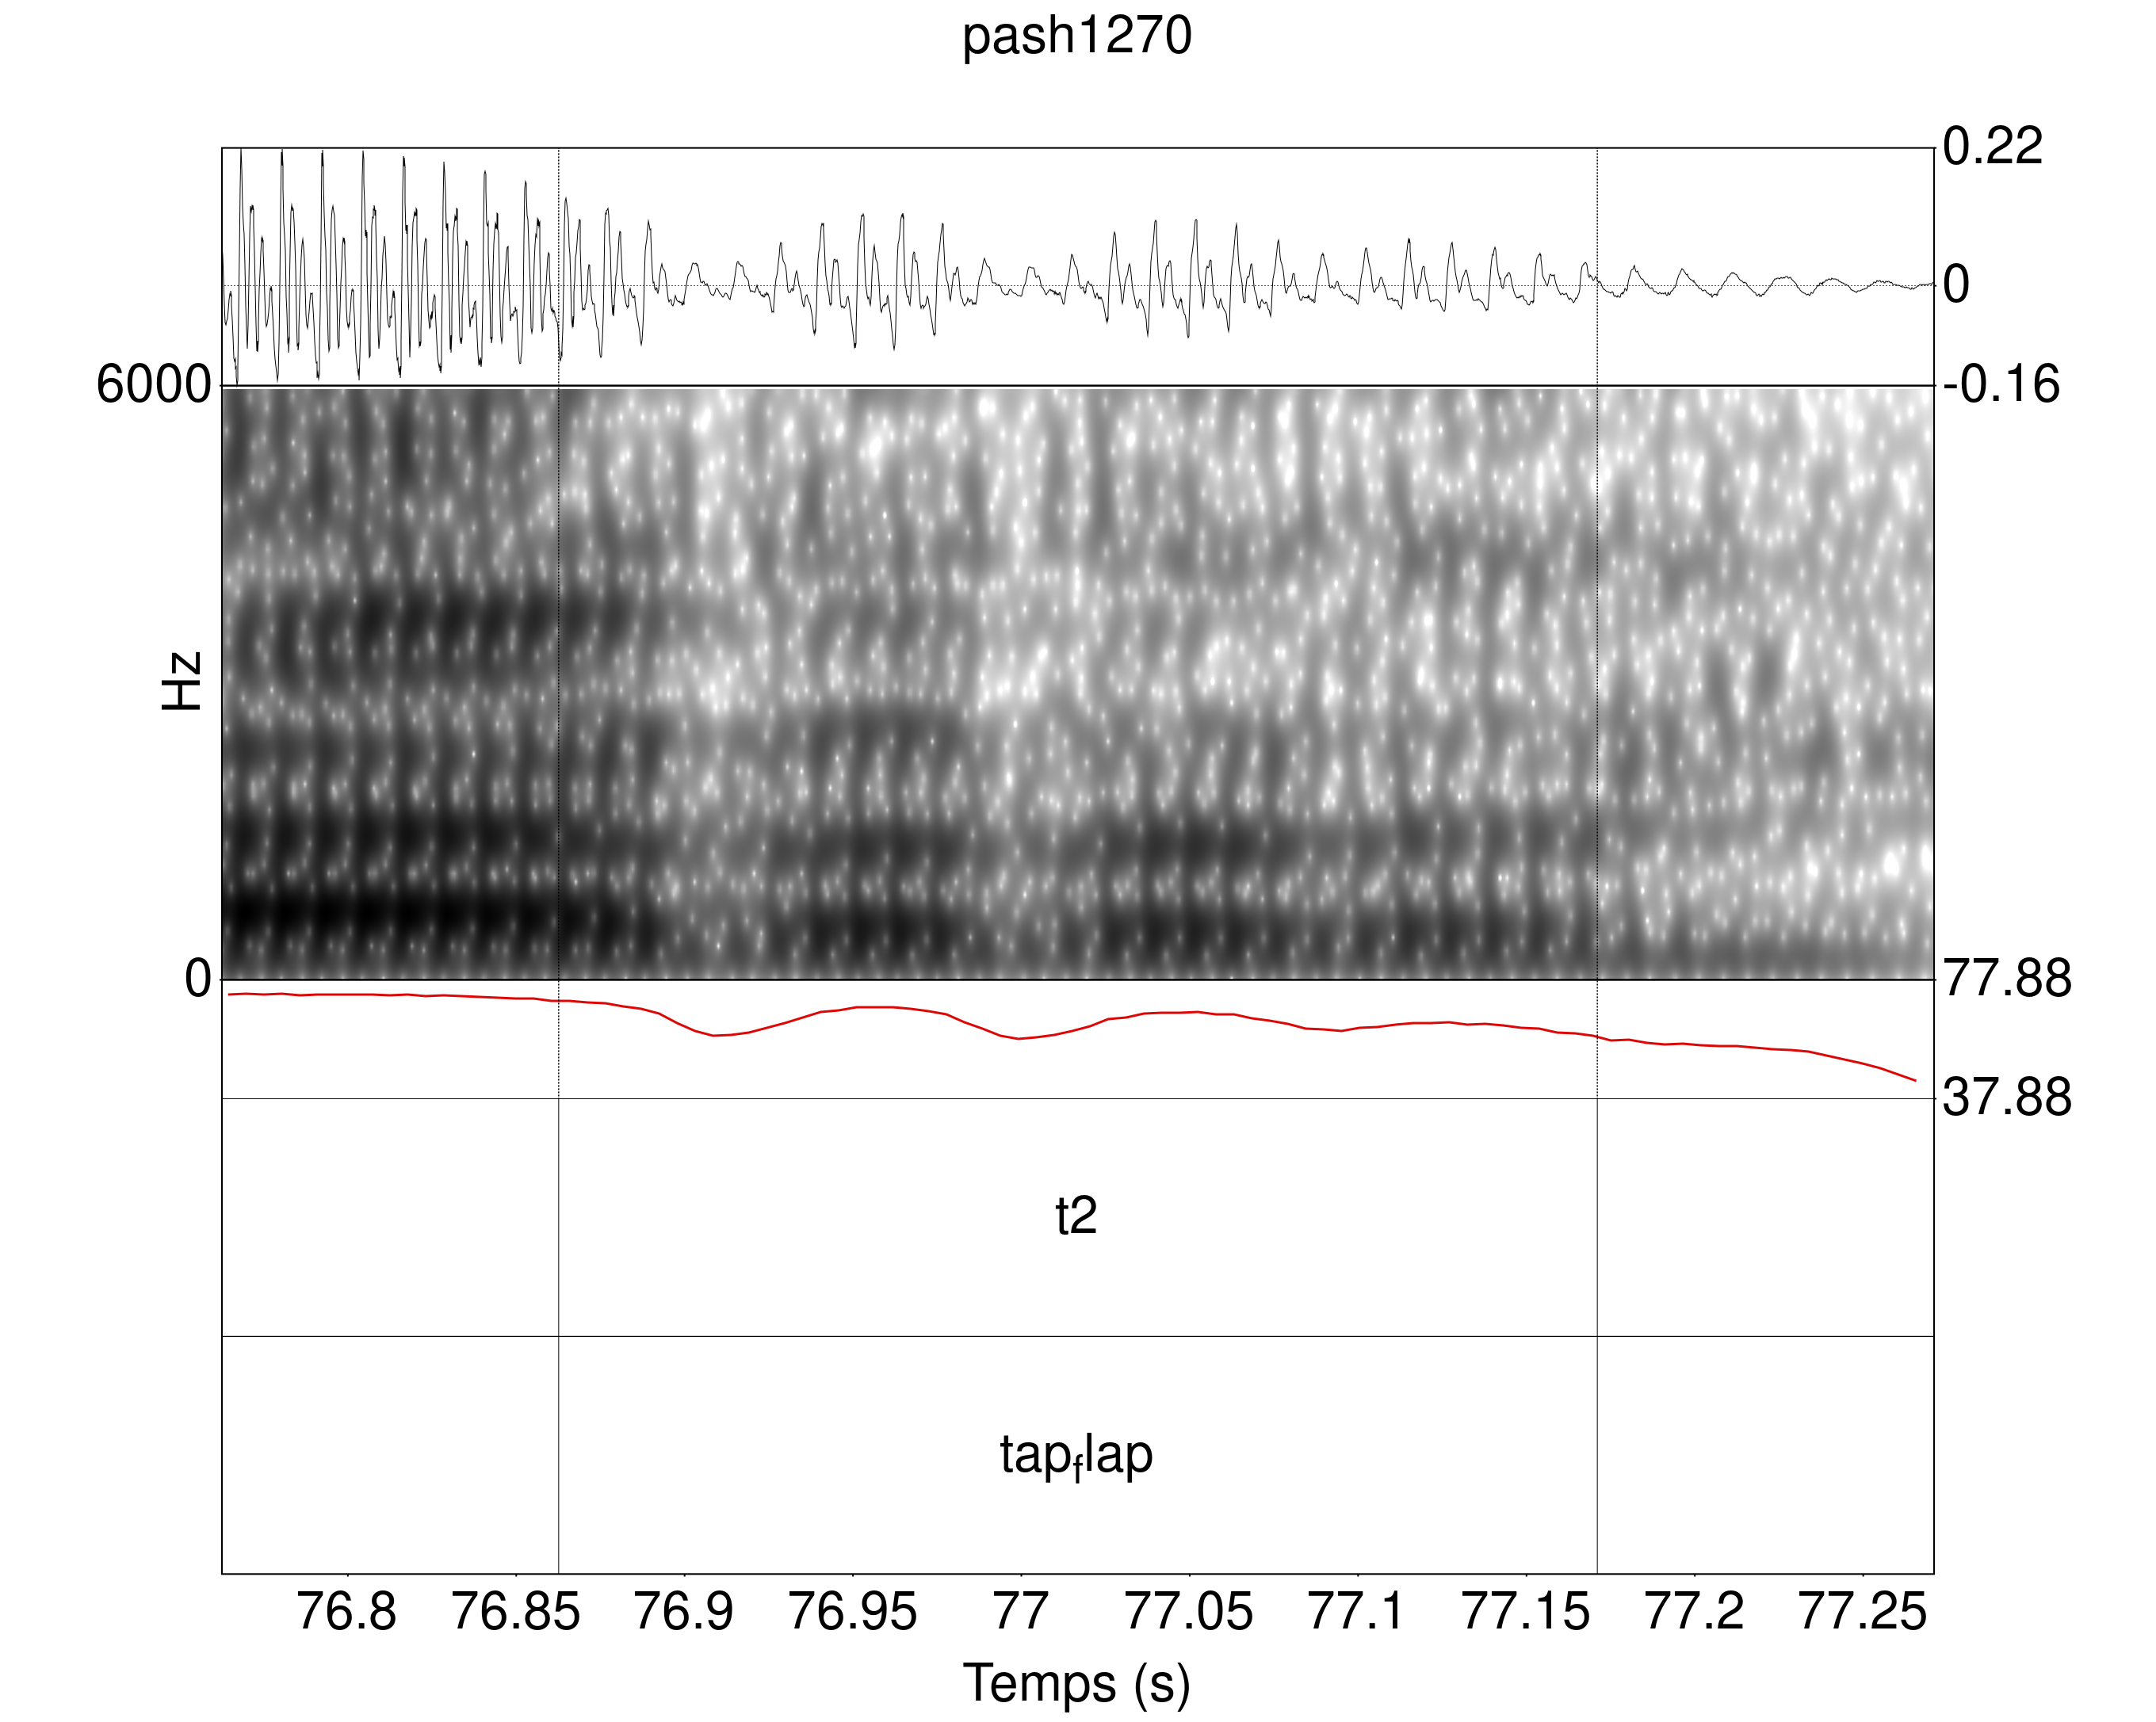
\includegraphics[width=0.45\linewidth]{substance/spectro_images/pash1270_1400_28}
	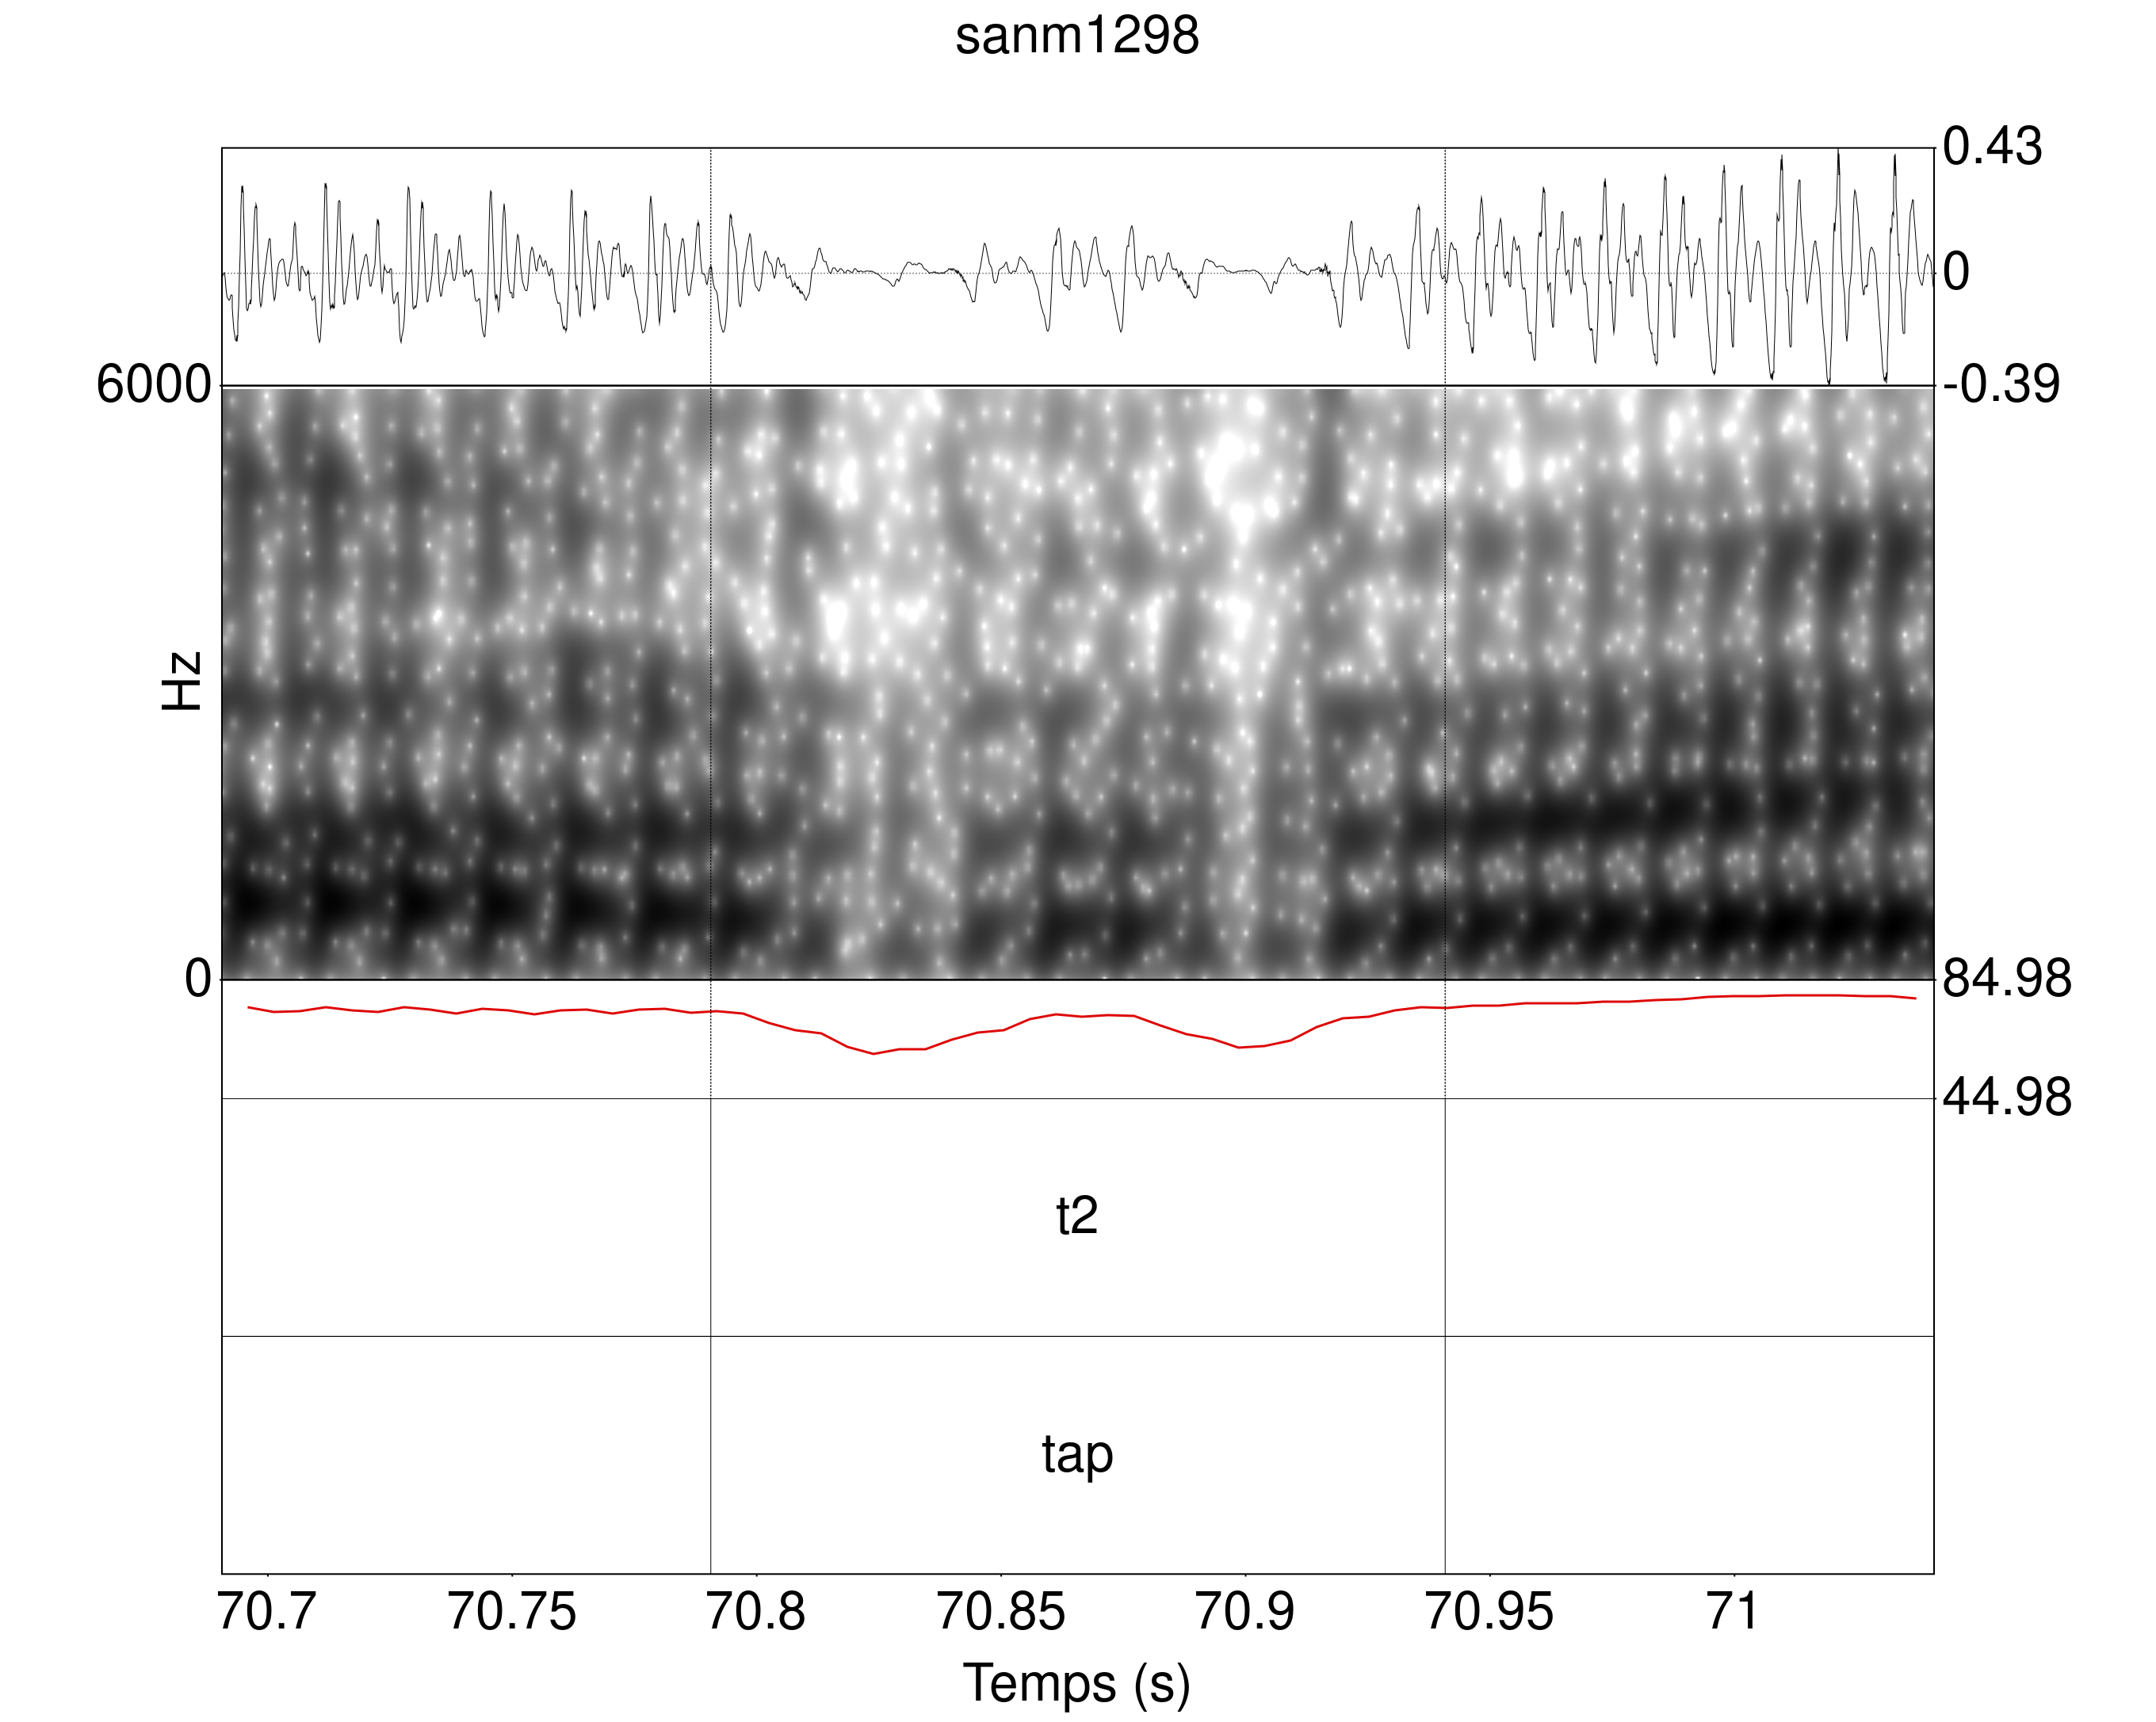
\includegraphics[width=0.45\linewidth]{substance/spectro_images/sanm1298_1558_6}
	\caption[Illustrations des \textg{t2} issus de 2 locuteurs/trices]{Illustrations des \textg{t2} issus de locuteurs/trices
		du pashai du sud est \glotto{pash1270} (2 occurrences sur 22 de t2 soit 9,1\% des trills) et 
		du galicien \glotto{gali1258} (2 occurrences sur 10 de t2 soit 100\% des trills). De haut en bas pour chacune des illustrations, nous avons l'oscillogramme, le spectrogramme, la courbe d'intensité, un palier intervallique avec la catégorie segmentée, et un palier intervallique comprenant le label descriptif du segment d'intérêt.}
	\label{fig:pashsanm}
\end{figure}


Finalement, nous nous intéressons aux segments labellisés comme \textg{trills/taps} et \textg{trills/flaps} avec quatre locuteurs/trices (\autoref{fig:variationtrillother}) dont deux produisent au moins un \textg{t2} comme illustré dans la \autoref{fig:platindo}.

\begin{figure}
	\centering
	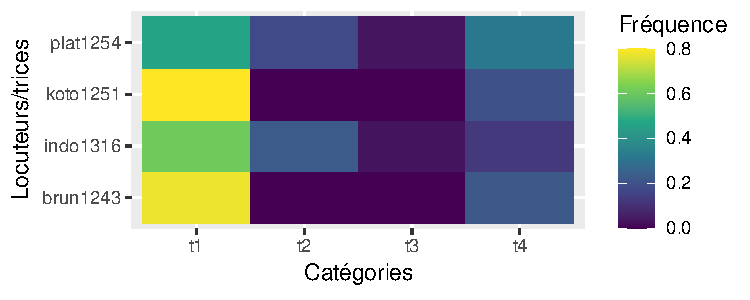
\includegraphics[width=0.45\linewidth]{substance/images/variation_trillother}
	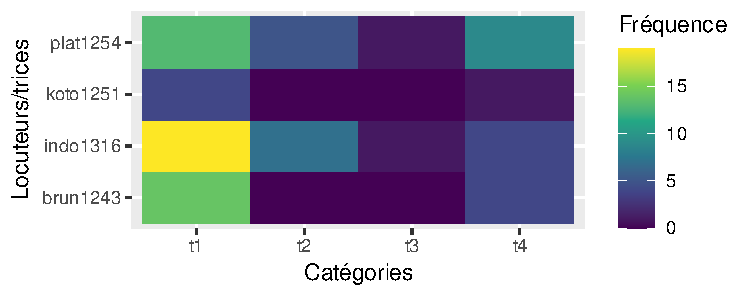
\includegraphics[width=0.45\linewidth]{substance/images/variation_trillother_abs}
	\caption[Fréquences relatives des différentes catégories illustrant la variation pour les segments ayant été catégorisés comme des \textg{trills/taps et trills/flaps}]{Fréquences relatives (à gauche) et absolues (à droite) des différentes catégories illustrant la variation pour les segments ayant été catégorisés par les auteurs des illustrations comme des \textg{trills/taps et trills/flaps}. Les fréquences sont calculées par ligne. Une case jaune est associée à une haute fréquence, cela veut dire que le/la locuteur/trice tend à produire une seule catégorie. Une case violette est associée à une catégorie non produite par le/la locuteur/trice.}
	\label{fig:variationtrillother}
\end{figure}


\begin{figure}
	\centering
	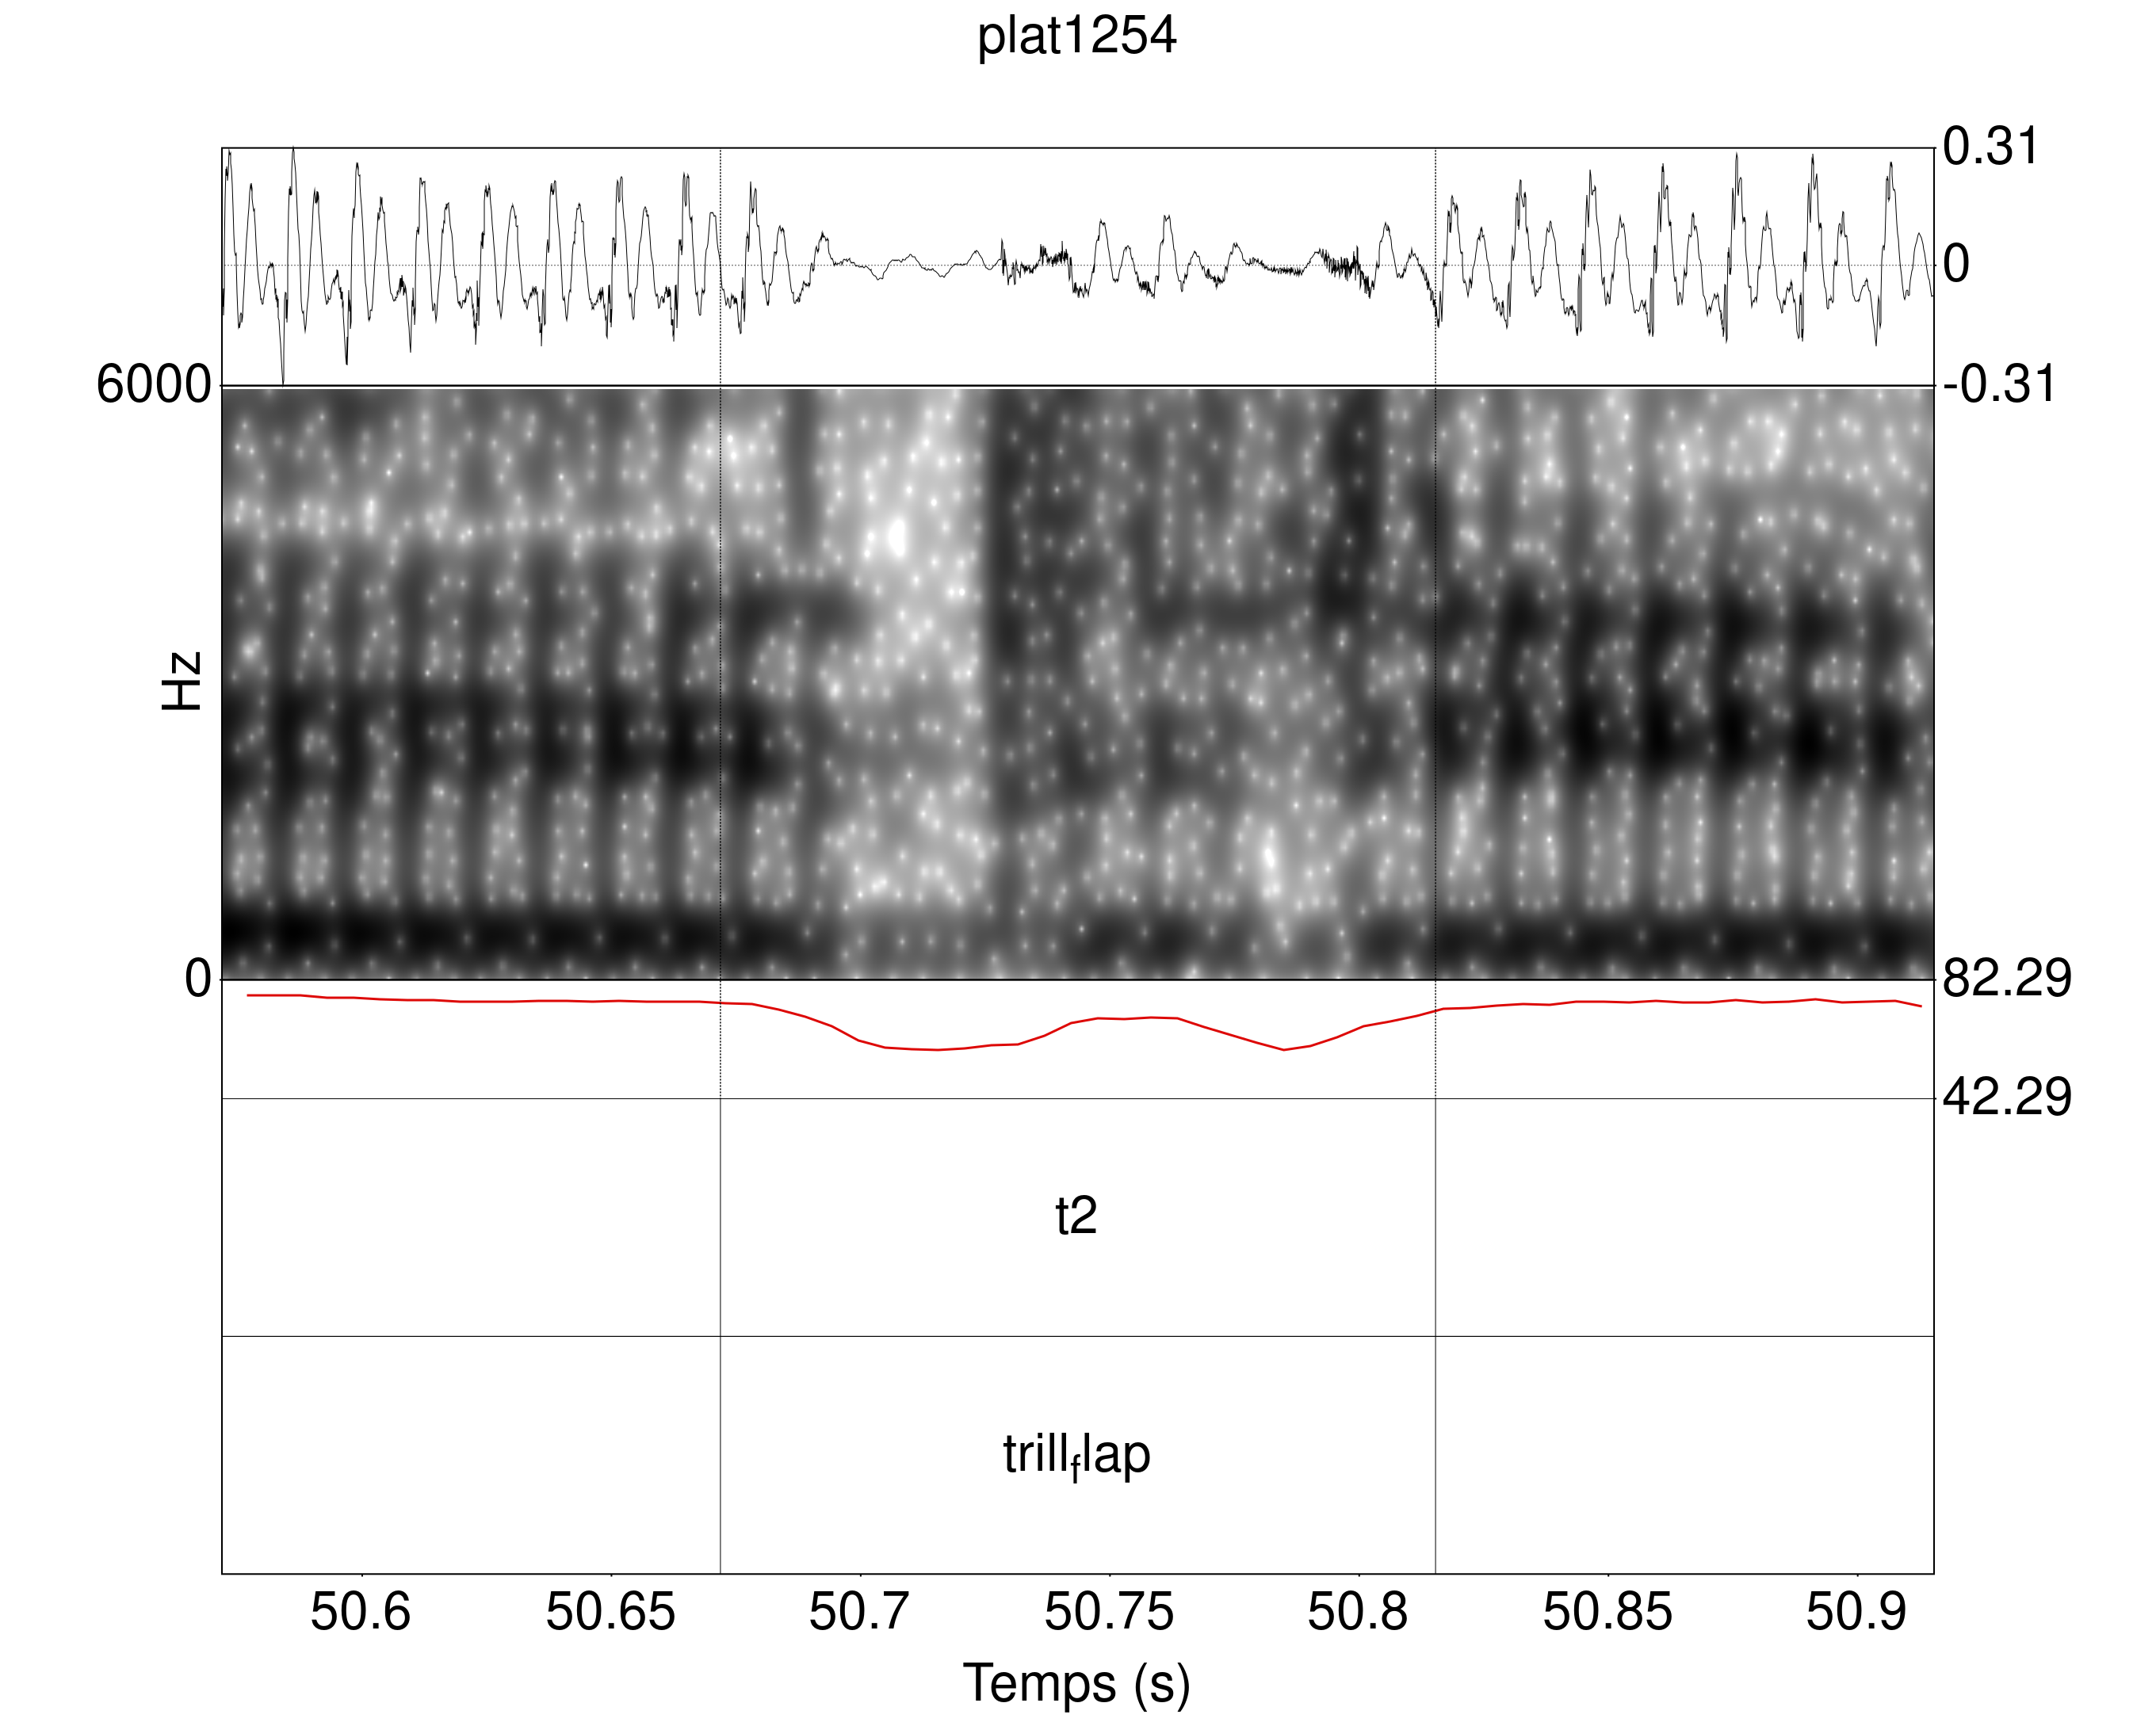
\includegraphics[width=0.45\linewidth]{substance/spectro_images/plat1254_1457_34}
	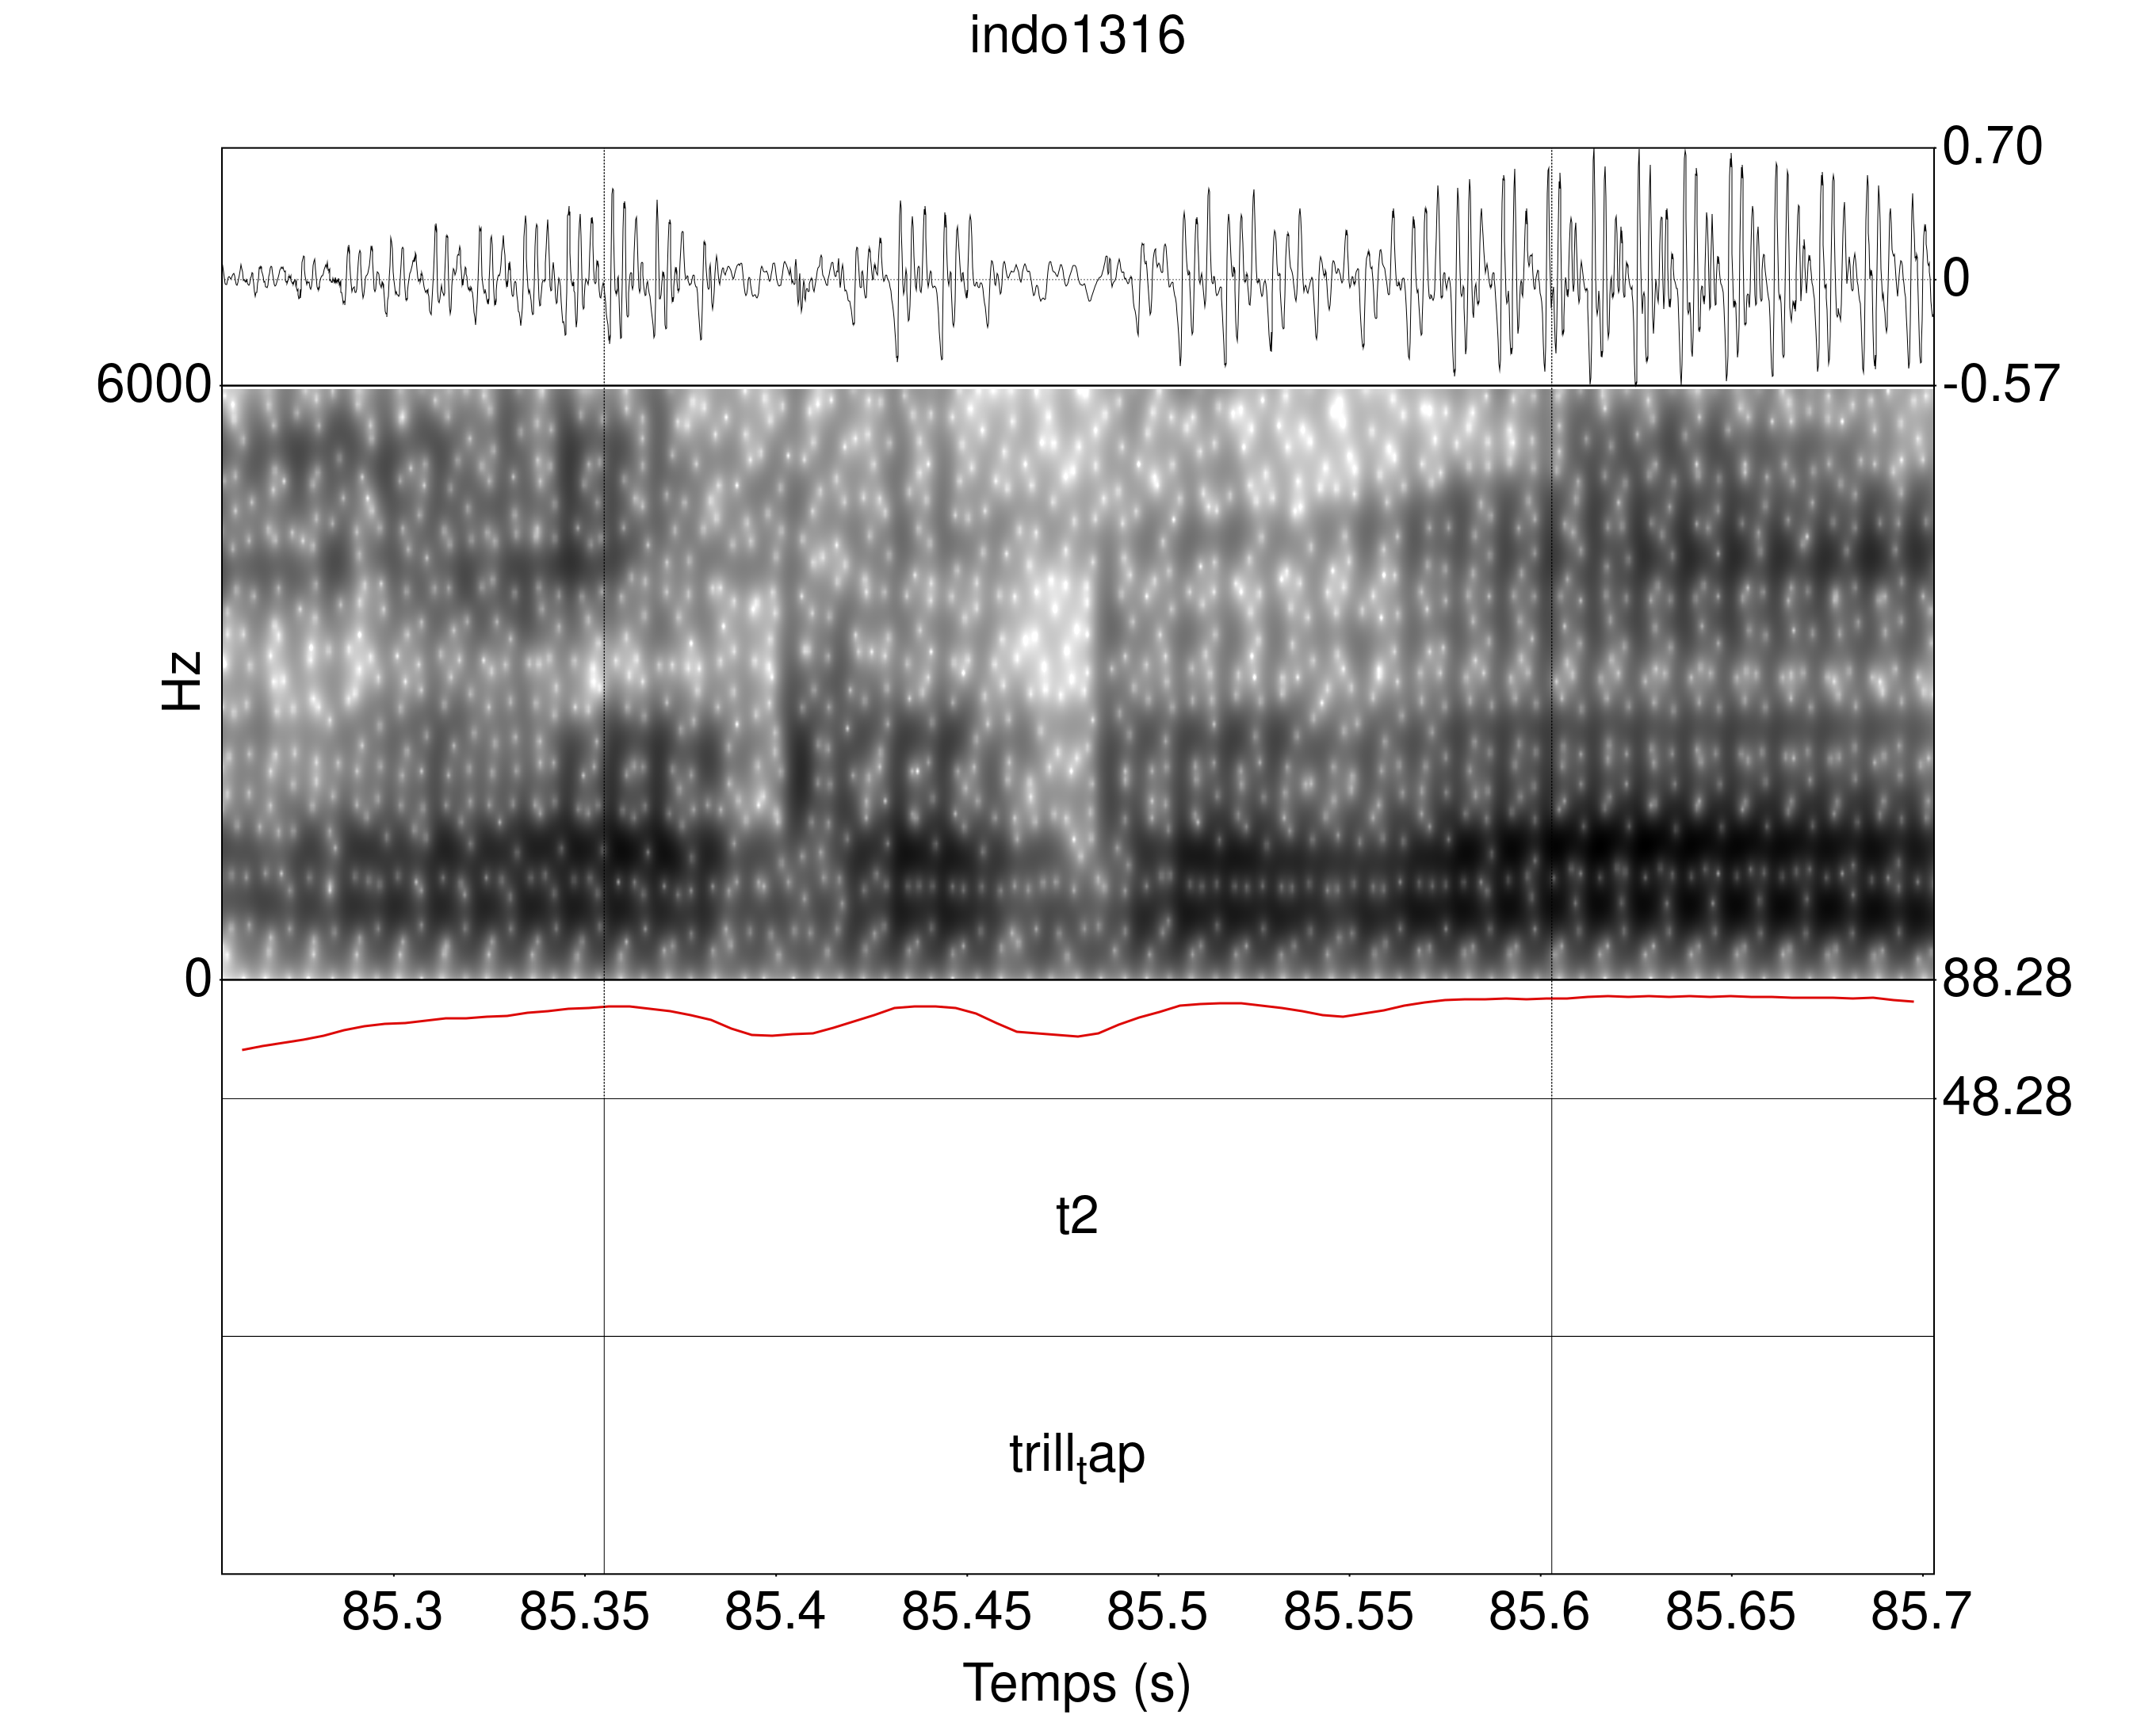
\includegraphics[width=0.45\linewidth]{substance/spectro_images/indo1316_858_34}
	\caption[Illustrations des \textg{t2} issus de locuteurs/trices]{Illustrations des \textg{t2} issus de locuteurs/trices
		de l'indonésien \glotto{indo1316} (7 occurrences sur 31 de t2 soit 22,6\% des trills) et 
		du malgache central \glotto{plat1254} (5 occurrences sur 28 de t2 soit 17,9\% des trills). De haut en bas pour chacune des illustrations, nous avons l'oscillogramme, le spectrogramme, la courbe d'intensité, un palier intervallique avec la catégorie segmentée, et un palier intervallique comprenant le label descriptif du segment d'intérêt.}
	\label{fig:platindo}
\end{figure}


\section{Deuxième étude : étude des composants des trills et taps}

La deuxième étude fait appel à une méthodologie plus précise que la première. Cette étude fait particulièrement attention à la segmentation. Du fait du peu de données, cette étude présente aussi des schémas idiosyncratiques. Les productions des rhotiques entre et au sein des individus varient.\\

Pour l'annotation, nous avons choisi de prendre en compte quatre unités de base pour la segmentation, que nous appellerons les \textg{éléments}.
Dans cette partie, nous illustrons les différents éléments ainsi que les motifs (les combinaisons d'éléments) avec des spectrogrammes. Nous considérons ces spectrogrammes comme \textg{prototypiques}, cependant, il faut prendre en compte que nous avons fait face à beaucoup de variation pendant le processus de segmentation et d'annotation. La mise en place des frontières sur le signal n'est pas toujours évidente. De plus, l'étape de segmentation a été mise en difficulté par la qualité des audios qui diffère d'une langue à une autre. Ainsi, dans certains cas, il a fallu s'appuyer plus sur la perception du son que sur la visualisation du signal acoustique\footnote{C'est le cas principalement des audios du mavea \glotto{mafe1237}.} (les TextGrids des différentes annotations sont mises à disposition sur \href{https://github.com/ranselme}{github.com/ranselme}).

Dans un premier temps, nous nous intéressons à la description des différents éléments, puis nous analysons la diversité des motifs obtenus. Nous nous concentrons sur la durée des motifs ainsi que sur les contextes des motifs les plus fréquents.

\subsection{Le \textg{o} : élément d'occlusion}

\begin{figure}
	\centering
	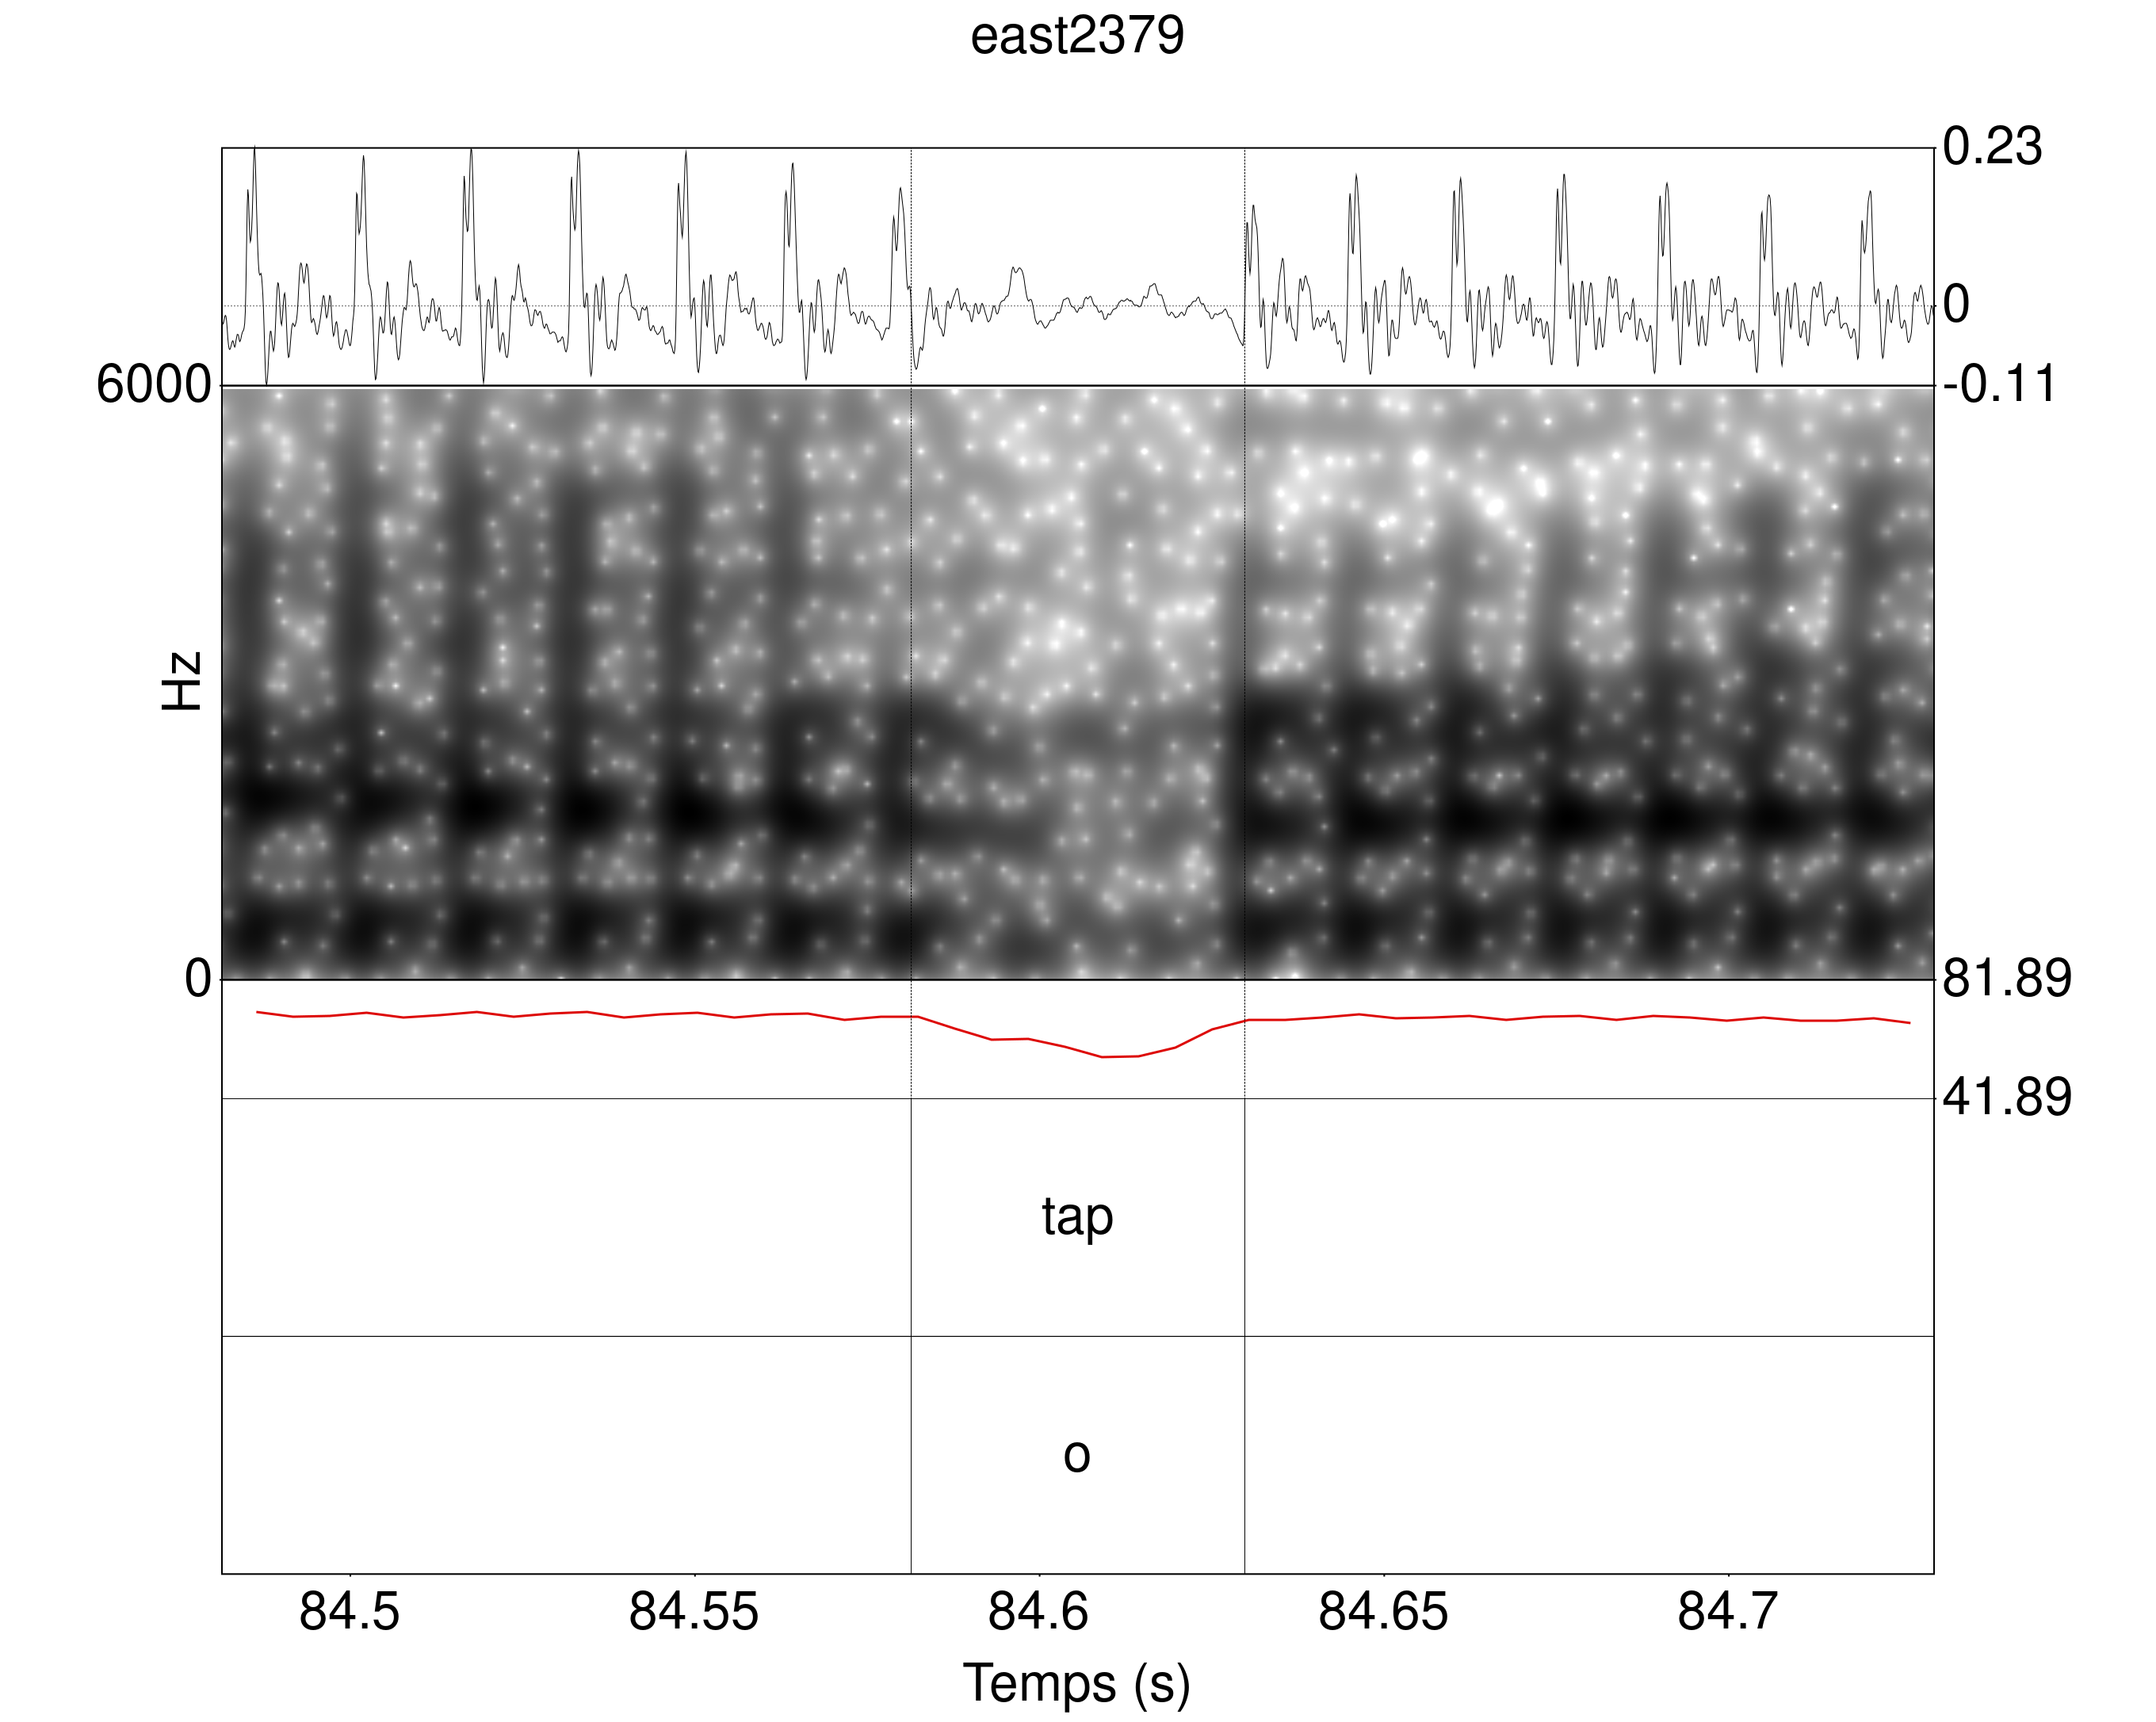
\includegraphics[width=0.8\linewidth]{substance/spectro_images/east2379_584_ɛrə}
	\caption[Illustration de l'élément \textg{o}]{Illustration de l'élément \textg{o} dans le contexte [ɛɾə] en arrernte central. De haut en bas, nous avons l'oscillogramme, le spectrogramme, la courbe d'intensité, un palier intervallique avec la catégorie segmentée, et un palier intervallique comprenant le label descriptif du segment d'intérêt.}
	\label{fig:east2379584r}
\end{figure}


Le premier élément que nous choisissons de décrire est l'élément \textg{o}. \textcite[65]{blecuaVibrantesEspanolManifestaciones2002} parle d'un élément correspondant à une phase brève de silence avec une barre de voisement. Cet élément peut se rencontrer indépendamment et former un segment à lui seul, ou peut se combiner avec d'autres éléments. \\

Sur le spectrogramme cet élément est reconnaissable par une baisse de l'énergie se traduisant par une zone plus \textg{blanche} (\autoref{fig:east2379584r}). De plus, on retrouve une baisse de l'intensité ainsi qu'une baisse de l'amplitude. Le signal n'est généralement pas périodique. Nous avons fait le choix de ne pas nous intéresser au voisement, ainsi nous ne faisons pas de distinction entre les \textg{o} voisés et les \textg{o} non-voisés.\\

La durée moyenne, tous contextes confondus, de l'élément \textg{o} est de 21,30 ms, sa médiane de 20,88 ms (minimum de 8,60 ms, maximum de 42,31 ms, IQR [écart interquartile] de 7,38 ms).


\subsection{Le \textg{b} : élément de relâchement (burst)}

\begin{figure}
	\centering
	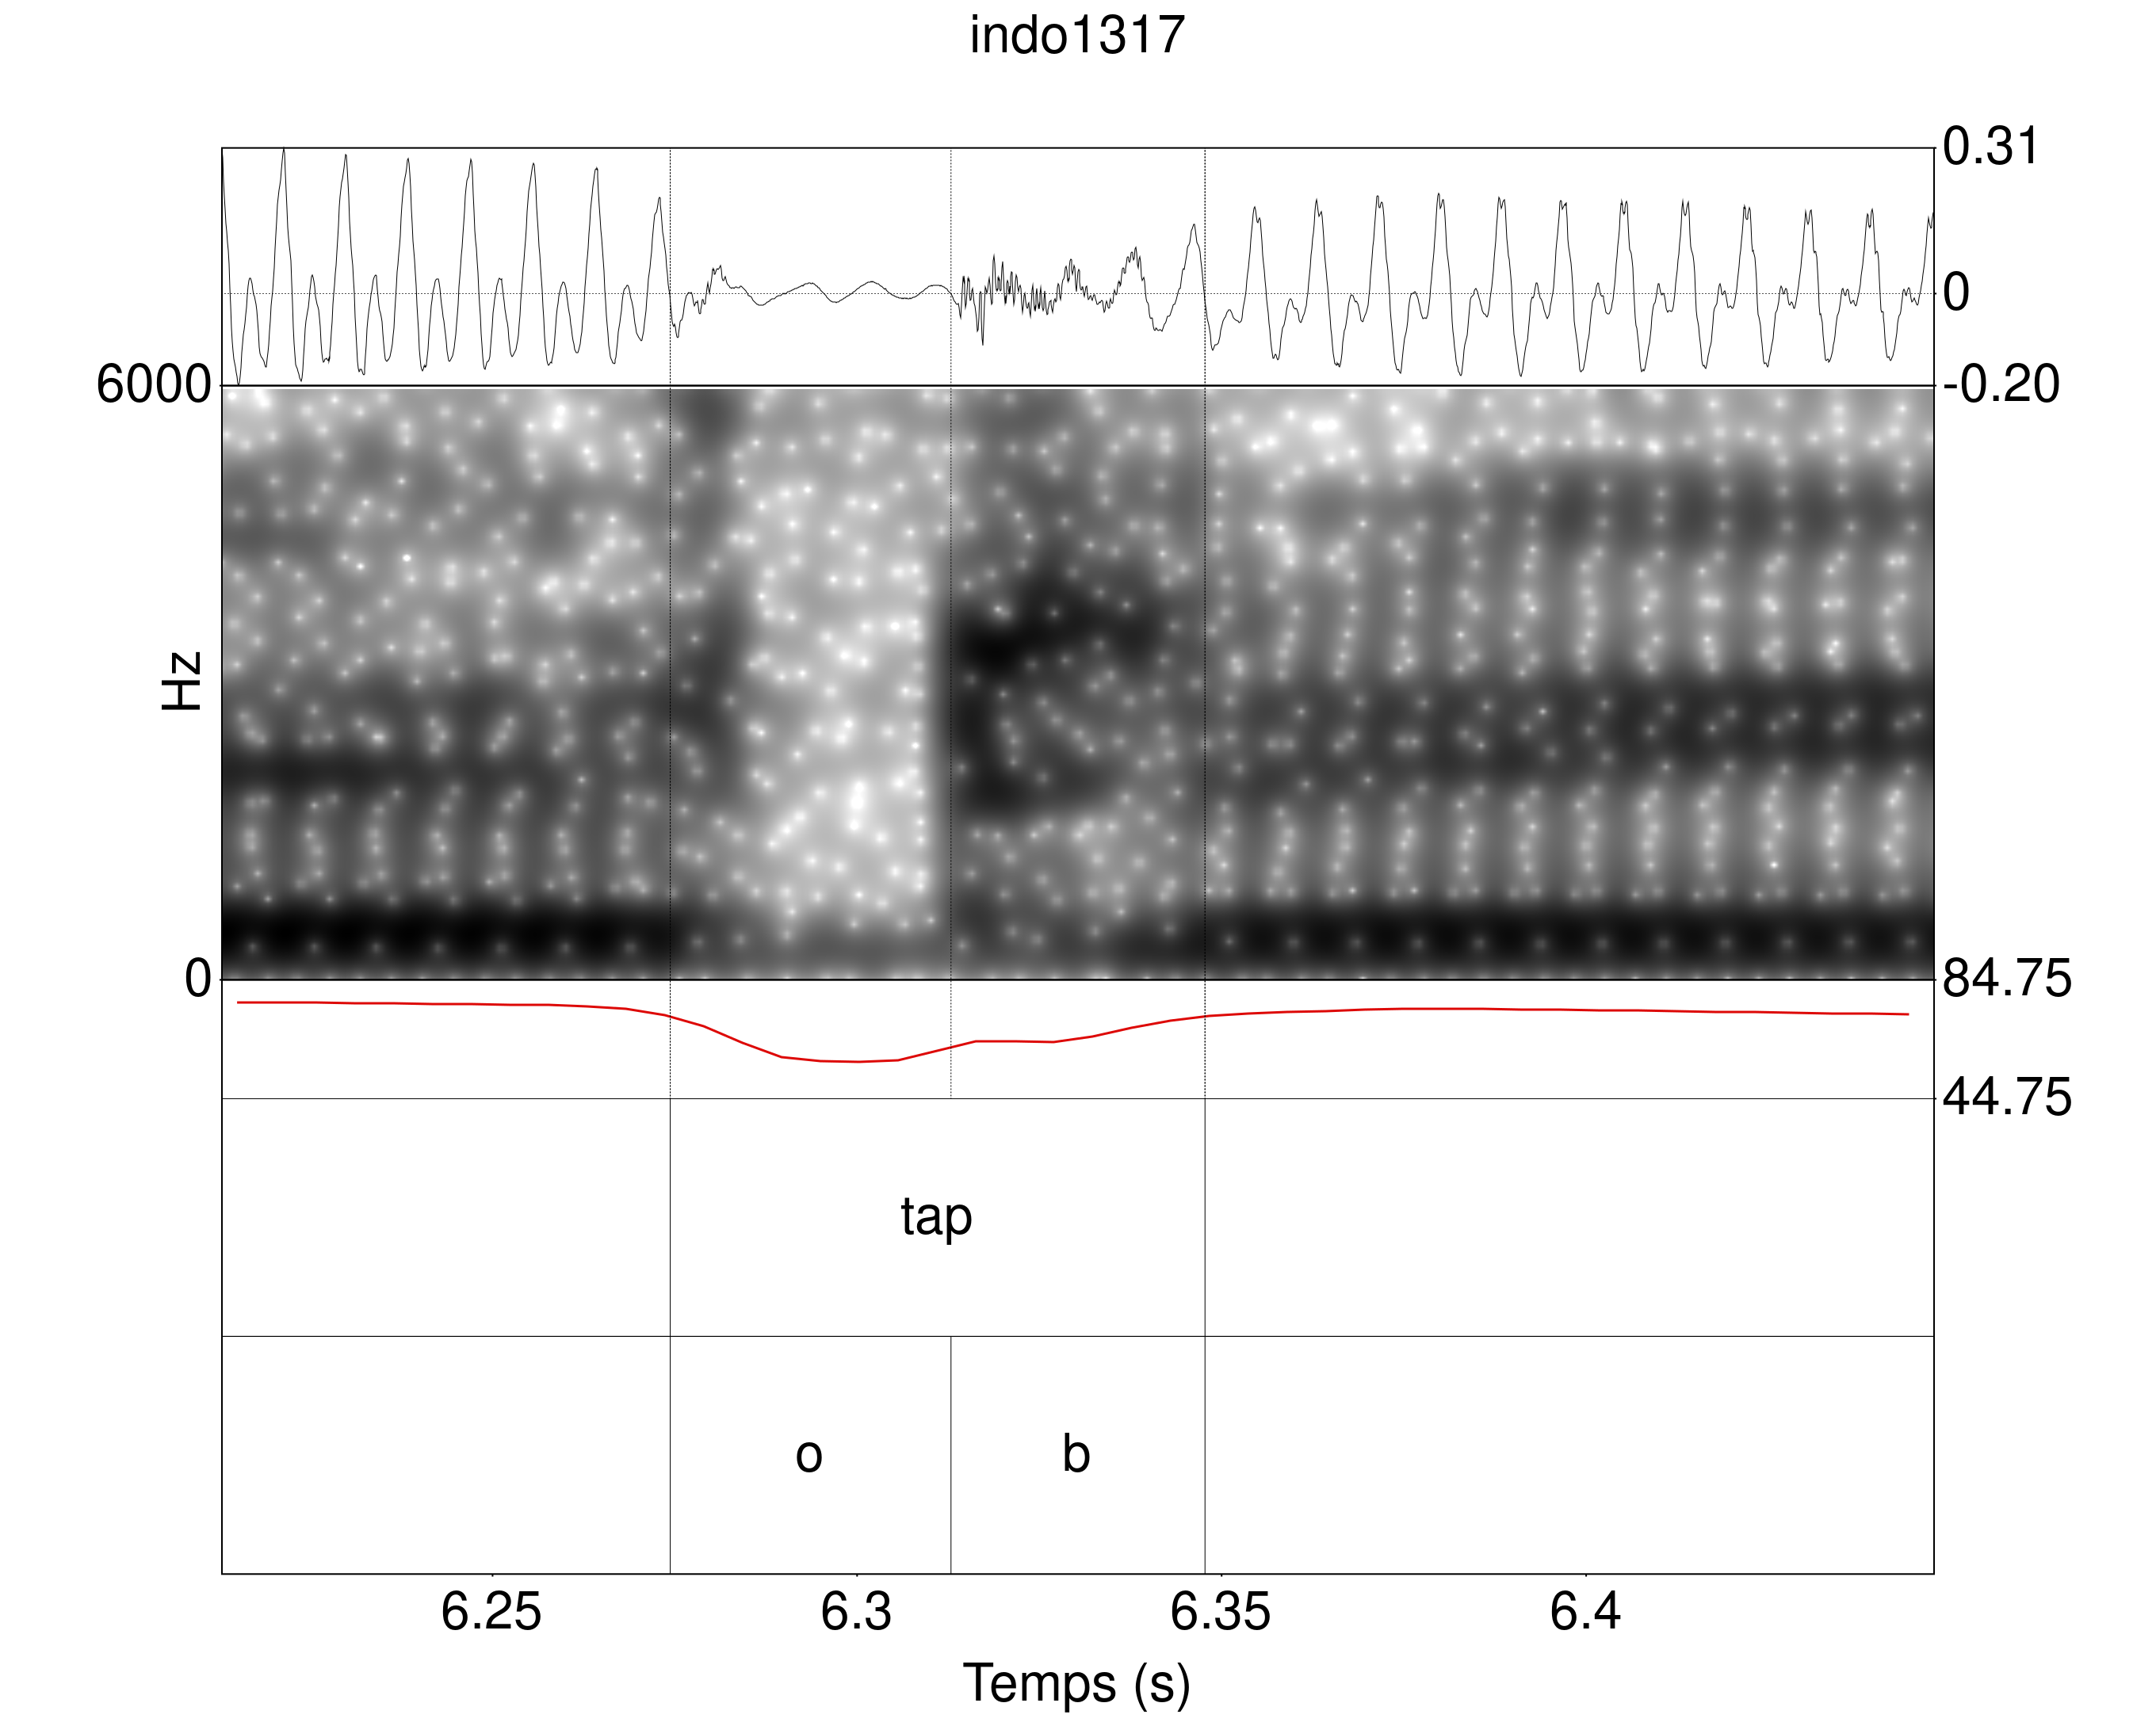
\includegraphics[width=0.8\linewidth]{substance/spectro_images/indo1317_477_}
	\caption[Illustration de l'élément \textg{b}]{Illustration de l'élément \textg{b} dans le contexte [ɯɾi] en indonésien des Bajau (Lombok de l'est). De haut en bas, nous avons l'oscillogramme, le spectrogramme, la courbe d'intensité, un palier intervallique avec la catégorie segmentée, et un palier intervallique comprenant le label descriptif du segment d'intérêt.}
	\label{fig:indo1317477}
\end{figure}

Le deuxième élément \textg{b} n'apparaît jamais en isolation et est systématiquement précédé d'un élément \textg{o} alors que le contraire n'est pas vrai. En effet, c'est la pression lors de l'occlusion qui entraîne cet élément \textg{b}. Il ne s'agit pas d'un élément vocalique mais d'un élément similaire à une occlusive avec une barre d'explosion (plus ou moins marquée) suivie d'un signal apériodique similaire (\autoref{fig:indo1317477}). \textcite[28]{skarnitzlPrinciplesPhoneticSegmentation2011} rappellent que les occlusives sont composées de plusieurs propriétés phonétiques inhérentes, parmi lesquelles on retrouve entre autres une fermeture complète au niveau du lieu d'articulation entraînant l'absence de structure formantique, et expliquant ainsi la présence d'un relâchement sous la forme de bruit d'explosion. \textcite[72]{skarnitzlPrinciplesPhoneticSegmentation2011} mentionnent que le cycle du [r] (à partir du spectrogramme qui accompagne sa description, on peut dire qu'ils illustrent leurs propos avec un motif \textg{ob}) peut être accompagné de \textg{plosion-like noise}.
Il n'y a donc pas de contre-indications à voir ce signal apériodique comme comparable au moment du relâchement dans une occlusive. On retrouve beaucoup d'énergie similaire à de la friction dans certains cas, avec parfois le début d'un signal périodique bruité.\\

\textcite[87]{blecuaVibrantesEspanolManifestaciones2002} mentionne cet élément dans sa section des taps en attaques complexes sans le catégoriser comme tel en parlant de certains éléments vocaliques : \textg{también se observan realizaciones en las que el elemento esvarabático es muy breve, e incluso podría llegar a confundirse con una barra de explosión}\footnote{Trad. : \textg{on observe aussi des réalisations dans lesquelles l'élément svarabhaktique est très bref, et qui pourrait être confondu avec une barre d'explosion}}. La mention de cet élément est aussi présente dans sa section sur les taps en codas (p. 152), sur les taps en position intervocalique (p. 198), ainsi que sur les trills en position intervocalique (cf. figure 96 page 238 reproduite en \autoref{fig:blecuafigure96}).\\

\begin{figure}
	\centering
	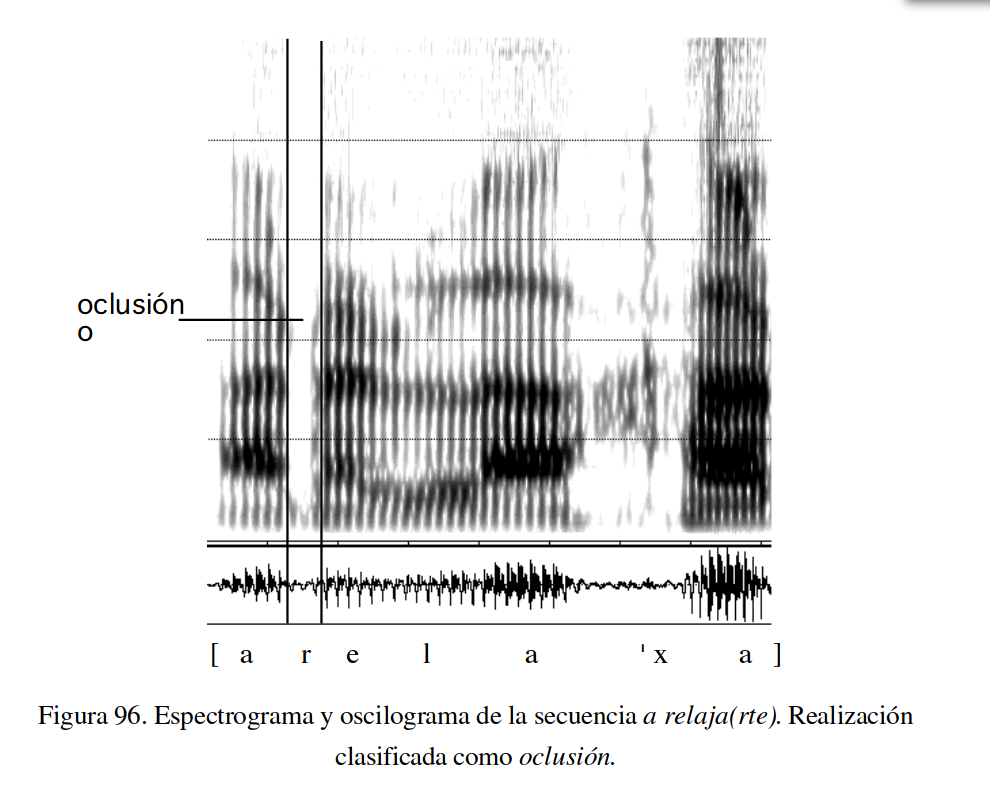
\includegraphics[width=0.8\linewidth]{substance/spectro_images/blecua_figure96}
	\caption[Illustration d'un élément \textg{o} par \textcite{blecuaVibrantesEspanolManifestaciones2002}]{Illustration d'un élément \textg{o} par \textcite[238]{blecuaVibrantesEspanolManifestaciones2002} où on retrouve aussi l'élément \textg{b}. [Trad : Spectrogramme et oscillogramme de la séquence \textit{a relaja(rte)}. Réalisation classifiée comme \textit{occlusion}].}
	\label{fig:blecuafigure96}
\end{figure}

La durée moyenne, tous contextes confondus, de l'élément \textg{b} est de 14,46 ms, sa médiane de 12,54 ms (minimum de 4,85 ms, maximum de 55,33 ms, IQR [écart interquartile] de 6,81 ms).\\



\subsection[Le \textg{a} : élément de constriction sans occlusion complète]{Le \textg{a} : élément de constriction sans occlusion complète (approximante)}

L'élément \textg{a} est un élément qui a été caractérisé par \textg{cualquier realización en la que se observe estructura formántica}\footnote{Trad. : \textg{n'importe quelle réalisation dans laquelle on observe une structure formantique}} \textcite[68]{blecuaVibrantesEspanolManifestaciones2002}. Pour qu'un élément appartienne à cette catégorie, il doit avoir une structure formantique au niveau du spectrogramme et un signal relativement similaire à un signal périodique (\autoref{fig:sout26041312r}). Nous avons aussi pris en compte une diminution de l'intensité nécessaire (même légère) pour que l'élément puisse être classé dans cette catégorie.

\begin{figure}
	\centering
	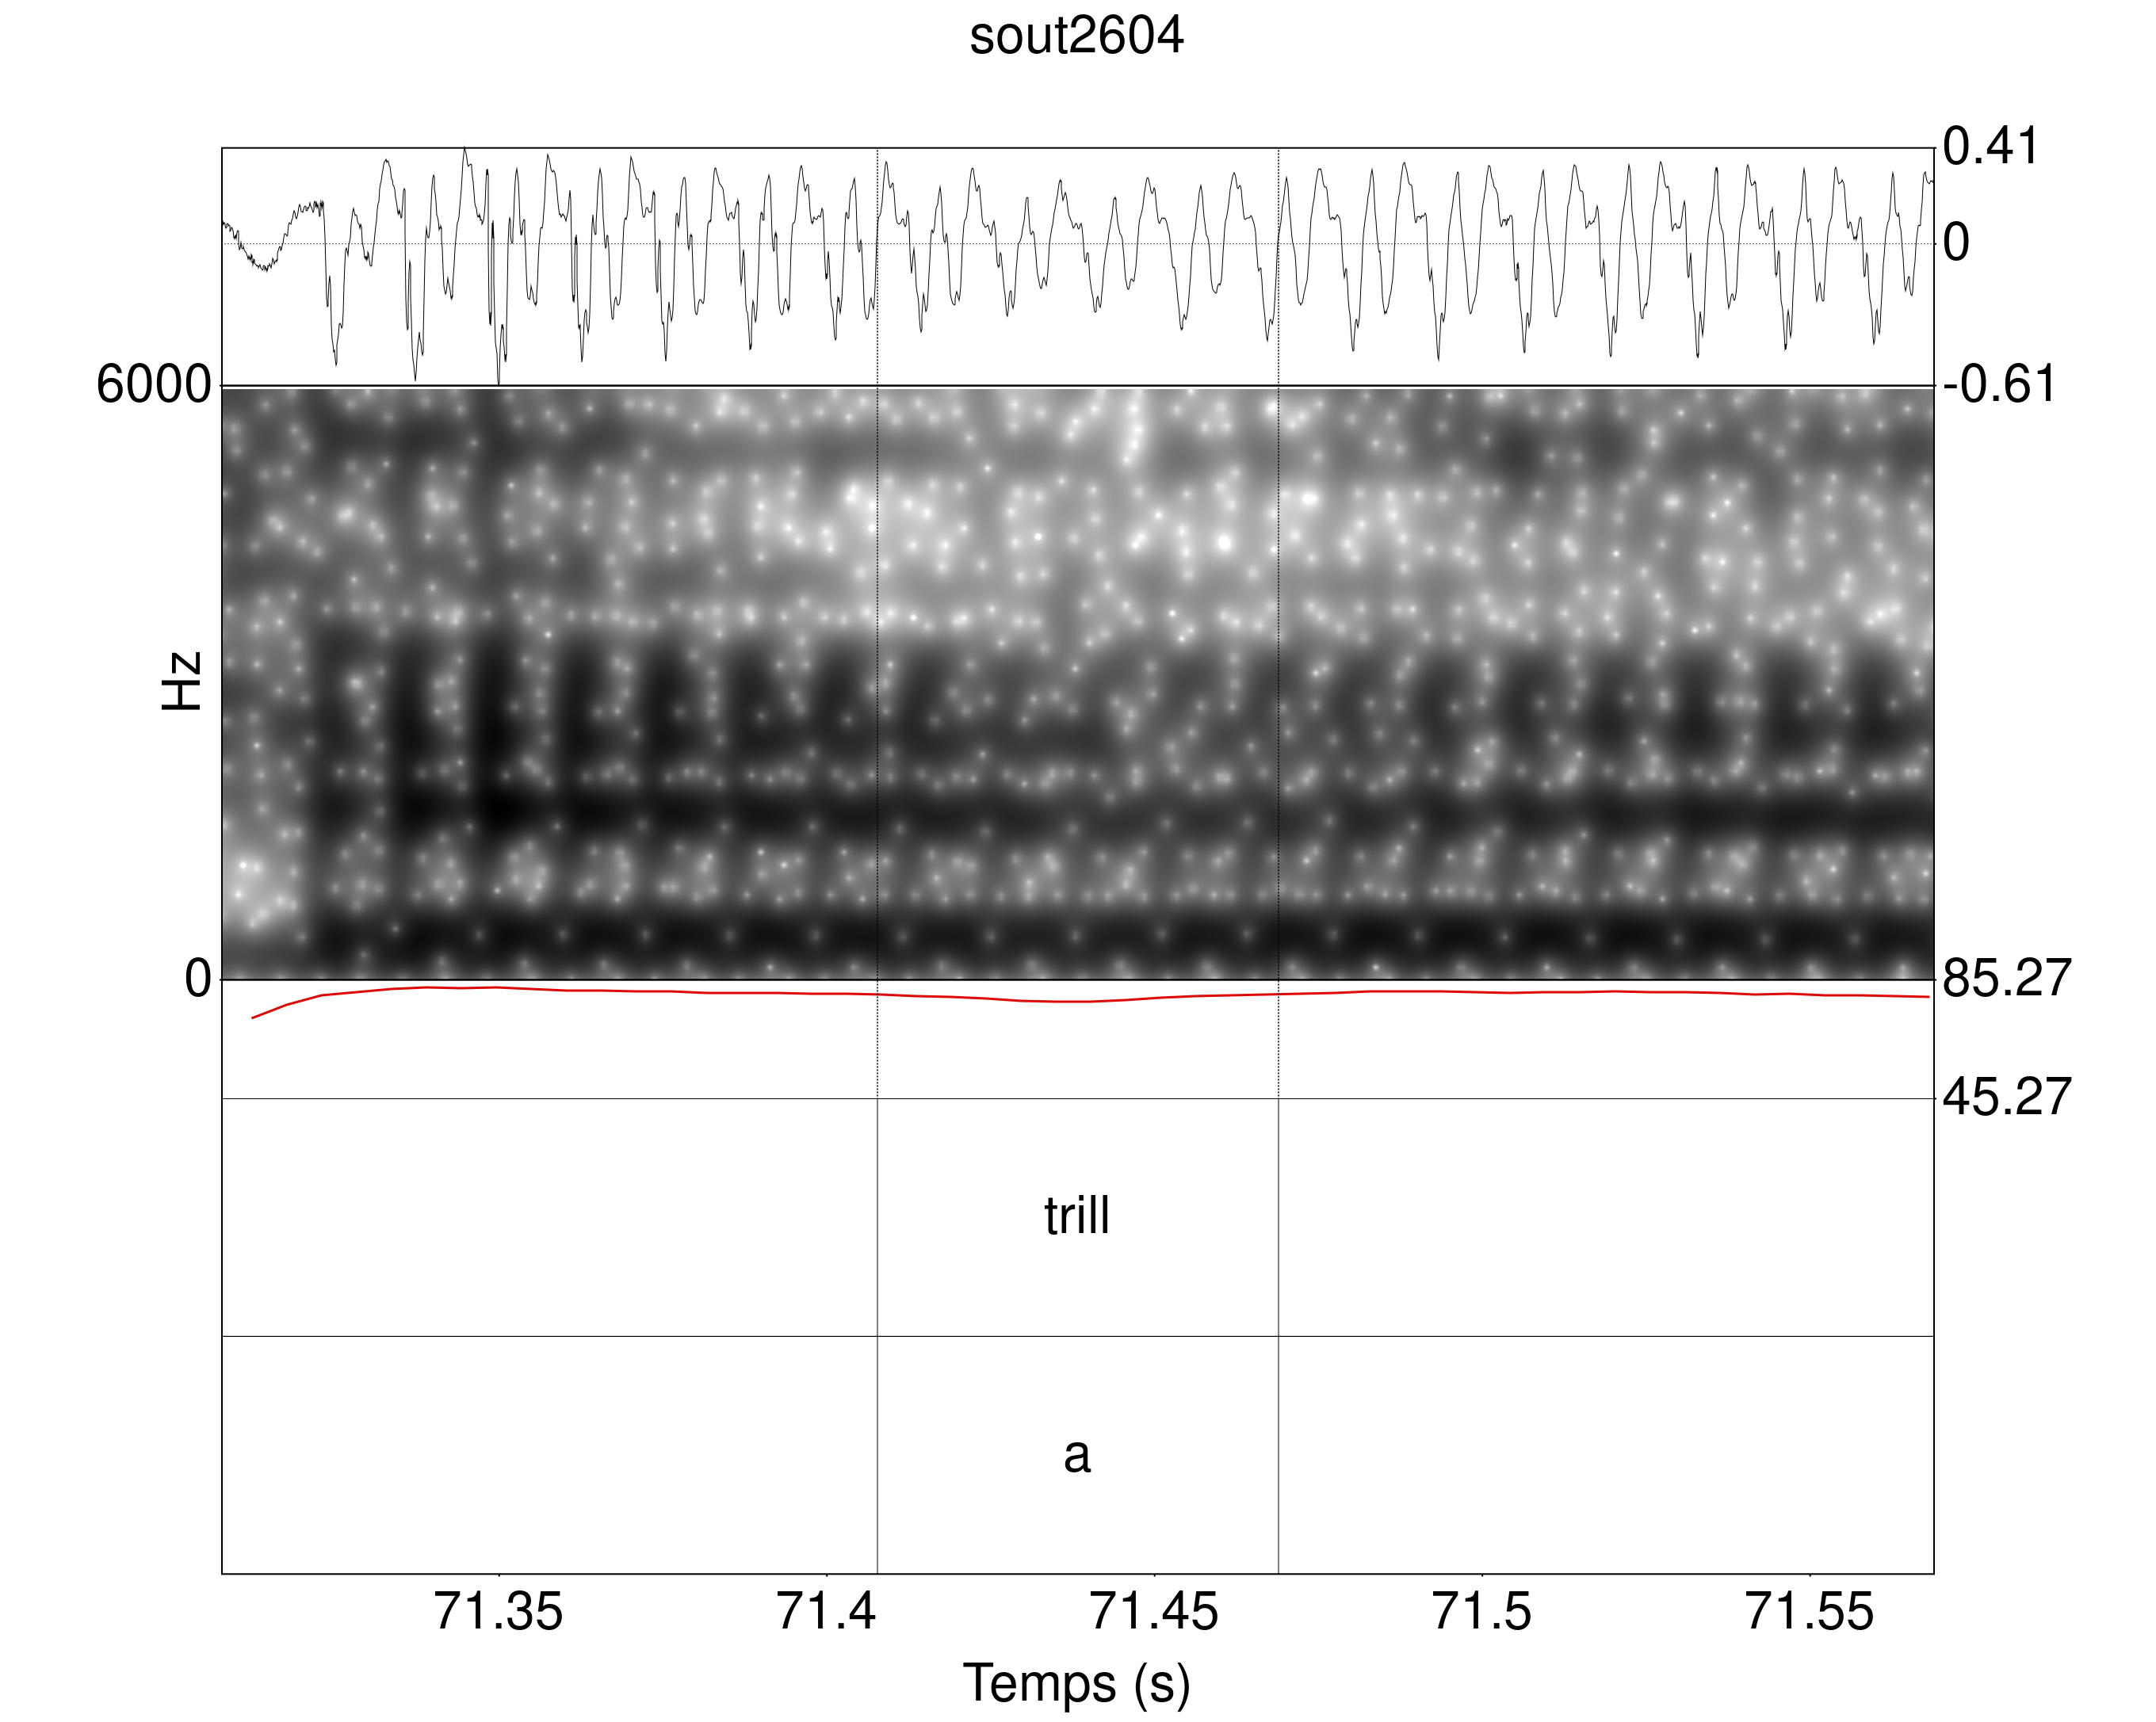
\includegraphics[width=0.7\linewidth]{substance/spectro_images/sout2604_1312_ɛrɛ}
	\caption[Illustration de l'élément \textg{a}]{Illustration de l'élément \textg{a} dans le contexte [ɛrɛ] en ukrainien. De haut en bas, nous avons l'oscillogramme, le spectrogramme, la courbe d'intensité, un palier intervallique avec la catégorie segmentée, et un palier intervallique comprenant le label descriptif du segment d'intérêt.}
	\label{fig:sout26041312r}
\end{figure}

La durée moyenne, tous contextes confondus, de l'élément \textg{a} est de 31,34 ms, sa médiane de 25,56 ms (minimum de 10,71 ms, maximum de 123,71 ms, IQR [écart interquartile] de 14,61 ms).


\subsection[Le \textg{c} : élément épenthétique vocalique]{Le \textg{c} : élément épenthétique vocalique\\ (élément \textg{svarabhaktique})}


Enfin, le dernier élément que nous avons décidé d'annoter est le \textg{c}. \textcite[38]{blecuaVibrantesEspanolManifestaciones2002} mentionne qu'il s'agit d'un élément avec des caractéristiques similaires à celles d'une voyelle courte, et qui possède donc des formants, bien que son intensité soit inférieure à celle de la voyelle suivante. Elle rapporte en citant Quilis (1970)\footnote{Quilis, A.(1970): \textg{El elemento esvarabático en los grupos [pr, br, tr...]}, dans \textit{Phonétique et linguistique romanes : Mélanges offerts à M.Georges Straka}, Lyon-Strasbourg, Societé de Linguistique Romane, I. pp. 99-104.} que sa durée est comprise entre 8 et 56 ms avec une durée moyenne de 32 ms.\\

\begin{figure}
	\centering
	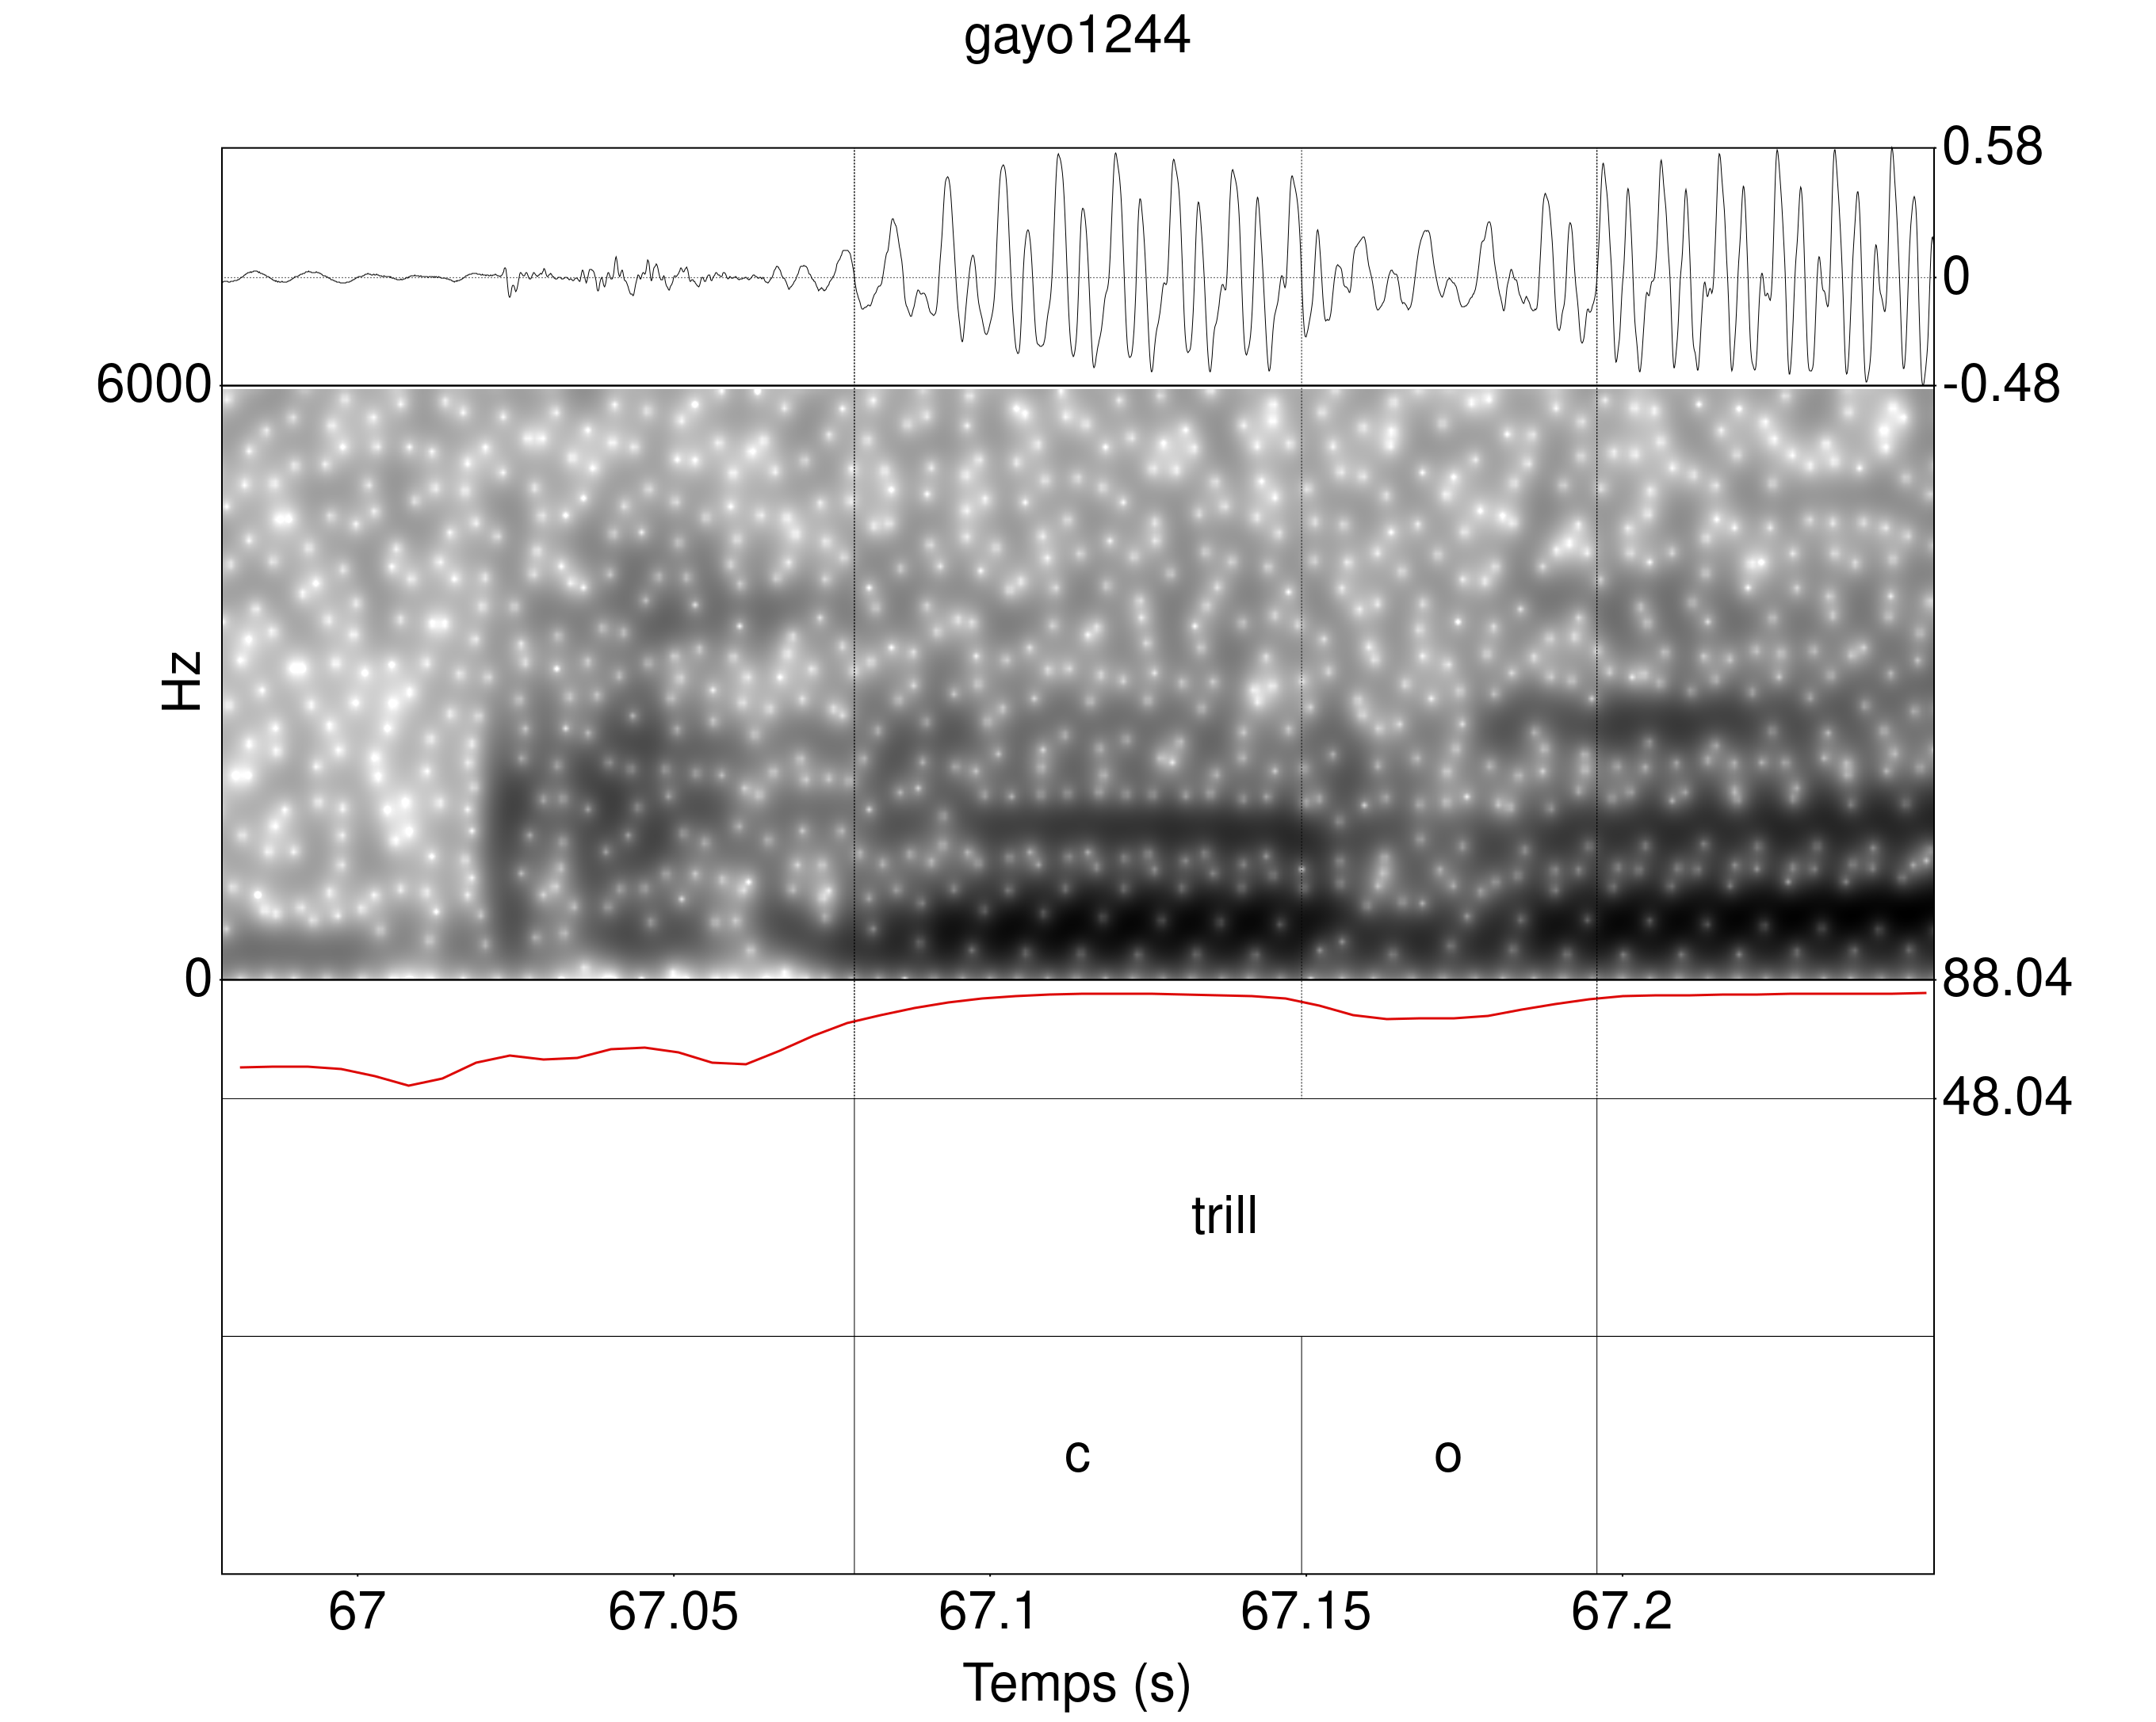
\includegraphics[width=0.8\linewidth]{substance/spectro_images/gayo1244_446_}
	\caption[Illustration de l'élément \textg{c}]{Illustration de l'élément \textg{c} dans le contexte [ˈkras] en gayo. De haut en bas, nous avons l'oscillogramme, le spectrogramme, la courbe d'intensité, un palier intervallique avec la catégorie segmentée, et un palier intervallique comprenant le label descriptif du segment d'intérêt.}
	\label{fig:gayo1244446}
\end{figure}

Il était parfois difficile de faire la différence entre un élément \textg{a} et un élément \textg{c}.
Par conséquent, nous avons essayé de nous référer à l'intensité qui a tendance à augmenter pour les éléments \textg{c} contrairement aux \textg{a} où elle diminue. Nous notons que certains cas restent problématiques à cause de structures non périodiques que nous avons tout de même choisi d'annoter comme \textg{c} (\autoref{fig:gayo1244446}).

La durée moyenne, tous contextes confondus, de l'élément \textg{c} est de 21,40 ms, sa médiane de 19,31 ms (minimum de 10,71 ms, maximum de 59,69 ms, IQR [écart interquartile] de 10,04 ms).

\section{Présentation des 18 langues segmentées et annotées}

Avec notre nouvelle méthode de segmentation et d'annotation, nous avons sélectionné 18 langues (\autoref{tab:description18langues}). La seule motivation sous-tendant ce choix est la présence de trills dans ces langues. Nous avons ensuite segmenté et annoté 400 segments. Le point commun de ces 18 langues est qu'elles ont toutes une \textit{Illustration of the IPA} contenant une transcription étroite et une transcription large. De ces transcriptions nous n'avons gardé que les transcriptions étroites que nous avons comparées avec le signal acoustique.\\

\begin{table}
	\centering
	%\resizebox{\linewidth}{!}{\csvautobooktabular{substance/tables/table_18langues.csv}}
	\resizebox{\linewidth}{!}{
\begin{tabular}{p{3.5cm} l l l l l}
\hline
Langue	&	Glottocode	&	Famille linguistique	&	Pays	&	Sexe	&	Age	\\
\hline
Afrikaans	&	afri1274	&	Indo-européen	&	Afrique du Sud	&	F	&	58	\\
Amarasi	&	koto1251	&	Austronésien	&	Timor	&	F	&	25	\\
Espagnol d’Argentine	&	amer1254	&	Indo-européen	&	Argentine	&	M	&	49	\\
Biélorusse	&	cent1954	&	Indo-européen	&	Biélorussie	&	M	&	30	\\
Malais du Brunei	&	brun1243	&	Austronésien	&	Brunei	&	F	&	22	\\
Sarde de Cagliari	&	meri1242	&	Indo-européen	&	Italie	&	F	&	73	\\
Castilian Spanish	&	cast1244	&	Indo-européen	&	Espagne	&	F	&	NA	\\
Arrernte central	&	east2379	&	Pama-Nyungan	&	Australie	&	F	&	NA	\\
Gayo	&	gayo1244	&	Austronésien	&	Indonésie	&	M	&	25	\\
Basque de Goizueta	&	basq1248	&	Basque	&	Espagne	&	F	&	NA	\\
Indonésien des Bajau (Lombok de l’est)	&	indo1317	&	Austronésien	&	Indonésie	&	F	&	22	\\
Trique d’Itunyoso	&	sanm1298	&	Oto-mangue	&	Mexique	&	M	&	27	\\
Kazakh	&	kaza1248	&	Turcique	&	Kazakhstan	&	F	&	30	\\
Mavea	&	mafe1237	&	Austronésien	&	Vanuatu	&	F	&	62	\\
Sasak, dialecte de Meno-Mené	&	meno1251	&	Austronésien	&	Indonésie	&	M	&	23	\\
Seenku	&	nort2820	&	Mandé	&	Mali	&	M	&	27	\\
Tamambo	&	malo1243	&	Austronésien	&	Vanuatu	&	F	&	27	\\
Ukrainien	&	sout2604	&	Indo-européen	&	Ukraine	&	M	&	38	\\
\hline
\end{tabular}
}
	\caption[Description des 18 langues.]{Description des 18 langues. Le seenku ne provient pas de l'échantillon des 73 langues car la rhotique n'est pas considérée comme phonémique dans la langue. La langue a été incluse grâce à la présence d'un [r] dans la transcription étroite fournie \parencite[18]{mcphersonSeenku2019}.}
	\label{tab:description18langues}
\end{table}

Les 18 langues appartiennent à sept familles linguistiques, avec une surreprésentation des langues indo-européennes et austronésiennes. Les enregistrements ont été réalisés sur sept hommes et onze femmes, avec un âge moyen de 37 ans et un âge médian de 27 ans (les données d'âge sont manquantes pour trois locutrices).\\


En ce qui concerne les différents labels descriptifs dans cet échantillon de langue, nous reportons les informations suivantes à partir des \textit{illustrations of the IPA} pour les langues correspondantes :

\begin{itemize}
	\item 5 segments sont issus de rhotiques décrites phonémiquement comme des approximantes /ɹ/
	\item 147 segments sont issus de rhotiques décrites phonémiquement comme des taps /ɾ/
	\item 217 segments sont issus de rhotiques décrites phonémiquement comme des trills /r/
	\item 6 segments sont issus de rhotiques décrites phonémiquement comme des trills palatalisés /rʲ/
	\item 23 segments sont issus de rhotiques décrites phonémiquement comme des trills/taps /r/\footnote{Les auteurs des deux illustrations qui mentionnent \textg{Trill/Tap} comme label descriptif pour la rhotique ont choisi d'utiliser le symbole <r>.}
	\item 2 segments sont issus de rhotiques décrites phonémiquement comme des trills géminés /rr/
\end{itemize}

Malgré la variation dans les labels descriptifs, nous n'allons pas considérer le niveau phonémique (le niveau spécifique à chaque langue) pour les descriptions acoustiques, pour nous concentrer uniquement sur les différences et les similitudes entre les motifs acoustiques. Nous avons eu accès aux différents contextes grâce aux transcriptions étroites fournies par les auteurs et autrices.\footnote{Nous avons choisi de reproduire les transcriptions en \autoref{chap:ann_trans} pour illustrer la variation. Toutes les transcriptions ne suivent pas intégralement les directives de l'Association de Phonétique Internationale, cependant, il s'agit d'une source d'information importante pour comprendre les contextes de production des différents segments.}
Nous mentionnerons ce niveau phonémique pour essayer d'apporter des éléments de réponses aux différences possibles entre ce que les auteurs des illustrations considèrent comme un trill et ce qu'ils considèrent comme un tap.



\subsection{Descriptions des différents motifs (combinaisons d'éléments) obtenus}

Au total, nous avons annoté 32 motifs avec les différents \textg{éléments} que nous avions étudiés.
Les rhotiques segmentées n'ont pas toutes le même nombre d'éléments. La \autoref{tab:tableelementsdiff} met en évidence la pluralité de la composition des éléments pour obtenir les différents motifs. 

\begin{table}
	\centering
	%\resizebox{0.7\linewidth}{!}{\csvautobooktabular{substance/tables/table_elements_diff.csv}}
	\resizebox{\linewidth}{!}{
\begin{tabular}{l l p{2cm} ||l l p{2cm}}
\hline
Segments	&	Fréquence	&	Nombre d’élément(s)	&	Segments	&	Fréquence	&	Nombre d’élément(s)	\\
\hline
a	&	30	&	1	&	cobc	&	1	&	4	\\
o	&	84	&	1	&	coca	&	1	&	4	\\
ca	&	1	&	2	&	obca	&	5	&	4	\\
co	&	23	&	2	&	obco	&	8	&	4	\\
oa	&	2	&	2	&	ocac	&	1	&	4	\\
ob	&	72	&	2	&	ocoa	&	2	&	4	\\
oc	&	29	&	2	&	ococ	&	9	&	4	\\
aca	&	1	&	3	&	obcob	&	4	&	5	\\
aco	&	1	&	3	&	obcoc	&	2	&	5	\\
cob	&	14	&	3	&	ocaca	&	2	&	5	\\
oba	&	2	&	3	&	ococa	&	4	&	5	\\
obc	&	46	&	3	&	ococo	&	3	&	5	\\
obo	&	1	&	3	&	cocaca	&	1	&	6	\\
oca	&	29	&	3	&	obcobc	&	2	&	6	\\
oco	&	17	&	3	&	obobob	&	1	&	6	\\
caca	&	1	&	4	&	obcobco	&	1	&	7	\\
\hline
\end{tabular}
}
	\caption[Fréquence des différents motifs acoustiques segmentés]{Fréquence des différents motifs segmentés.}
	\label{tab:tableelementsdiff}
\end{table}

\begin{figure}
	\centering
	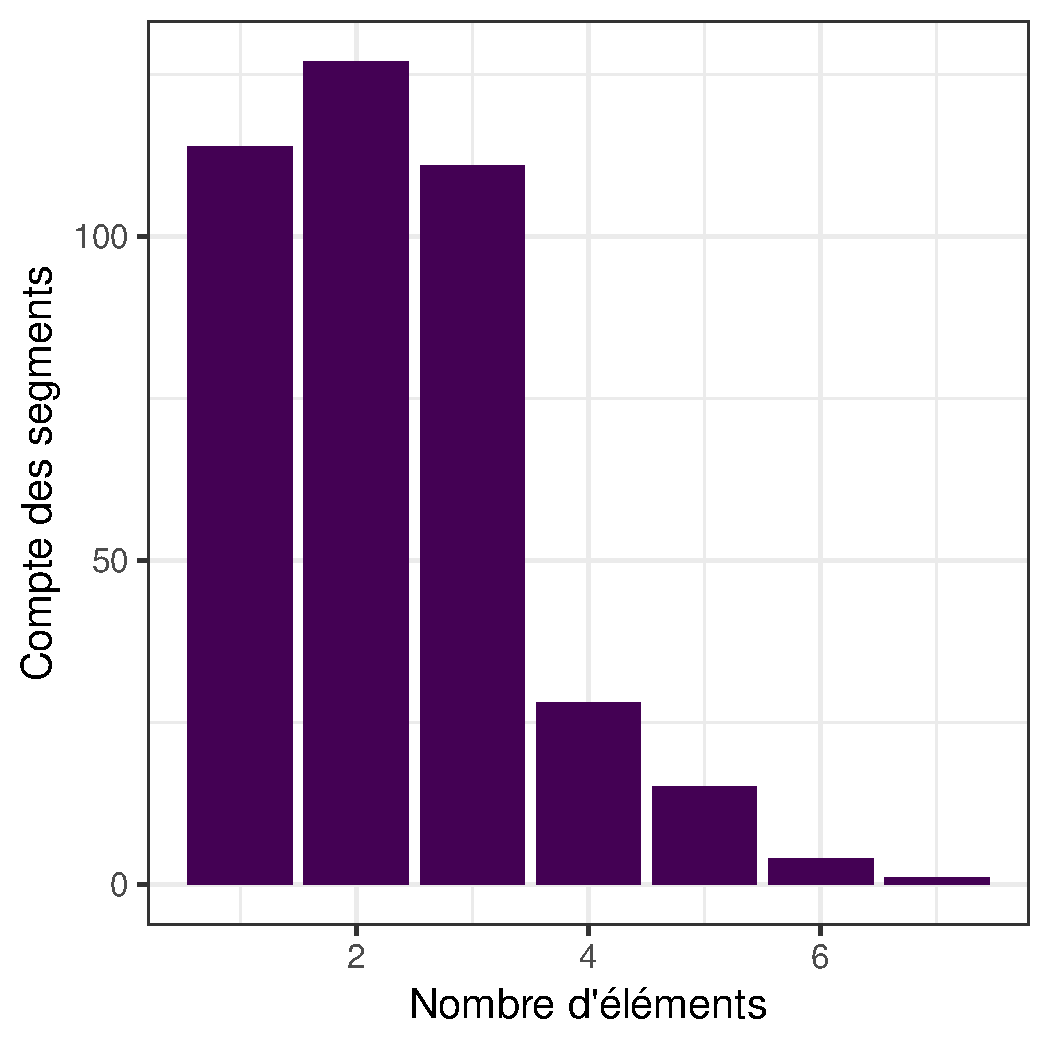
\includegraphics[width=0.45\linewidth]{substance/images/nb_elements}
	\caption[Compte des segments en fonction du nombre d'éléments]{Compte des segments en fonction du nombre d'éléments.}
	\label{fig:nbelements}
\end{figure}


La \autoref{fig:nbelements} permet de mettre en évidence que les segments annotés se composent principalement de un, deux ou trois éléments. Lorsque le segment possède un élément, il s'agit soit d'un \textg{a} soit d'un \textg{o}. Bien que les voyelles rhotiques existent, nous avons fait le choix de ne pas en annoter. Ainsi l'élément \textg{c} est obligatoirement accompagné d'un \textg{a} ou d'un \textg{o}.
Certains motifs sont plus présents, et plus un motif est composé d'éléments, moins il est fréquent. De tous les motifs annotés, nous n'avons qu'une occurrence de motif à sept éléments alors que nous avons 114 occurences de motifs à un élément.\\

L'élément \textg{b} apparaît dans 39,75\% des cas, il y a donc fréquemment dans nos données un vrai contact avec une barre d'explosion et un relâchement, bien que ce contact soit de courte durée.\\

\begin{figure}
	\centering
	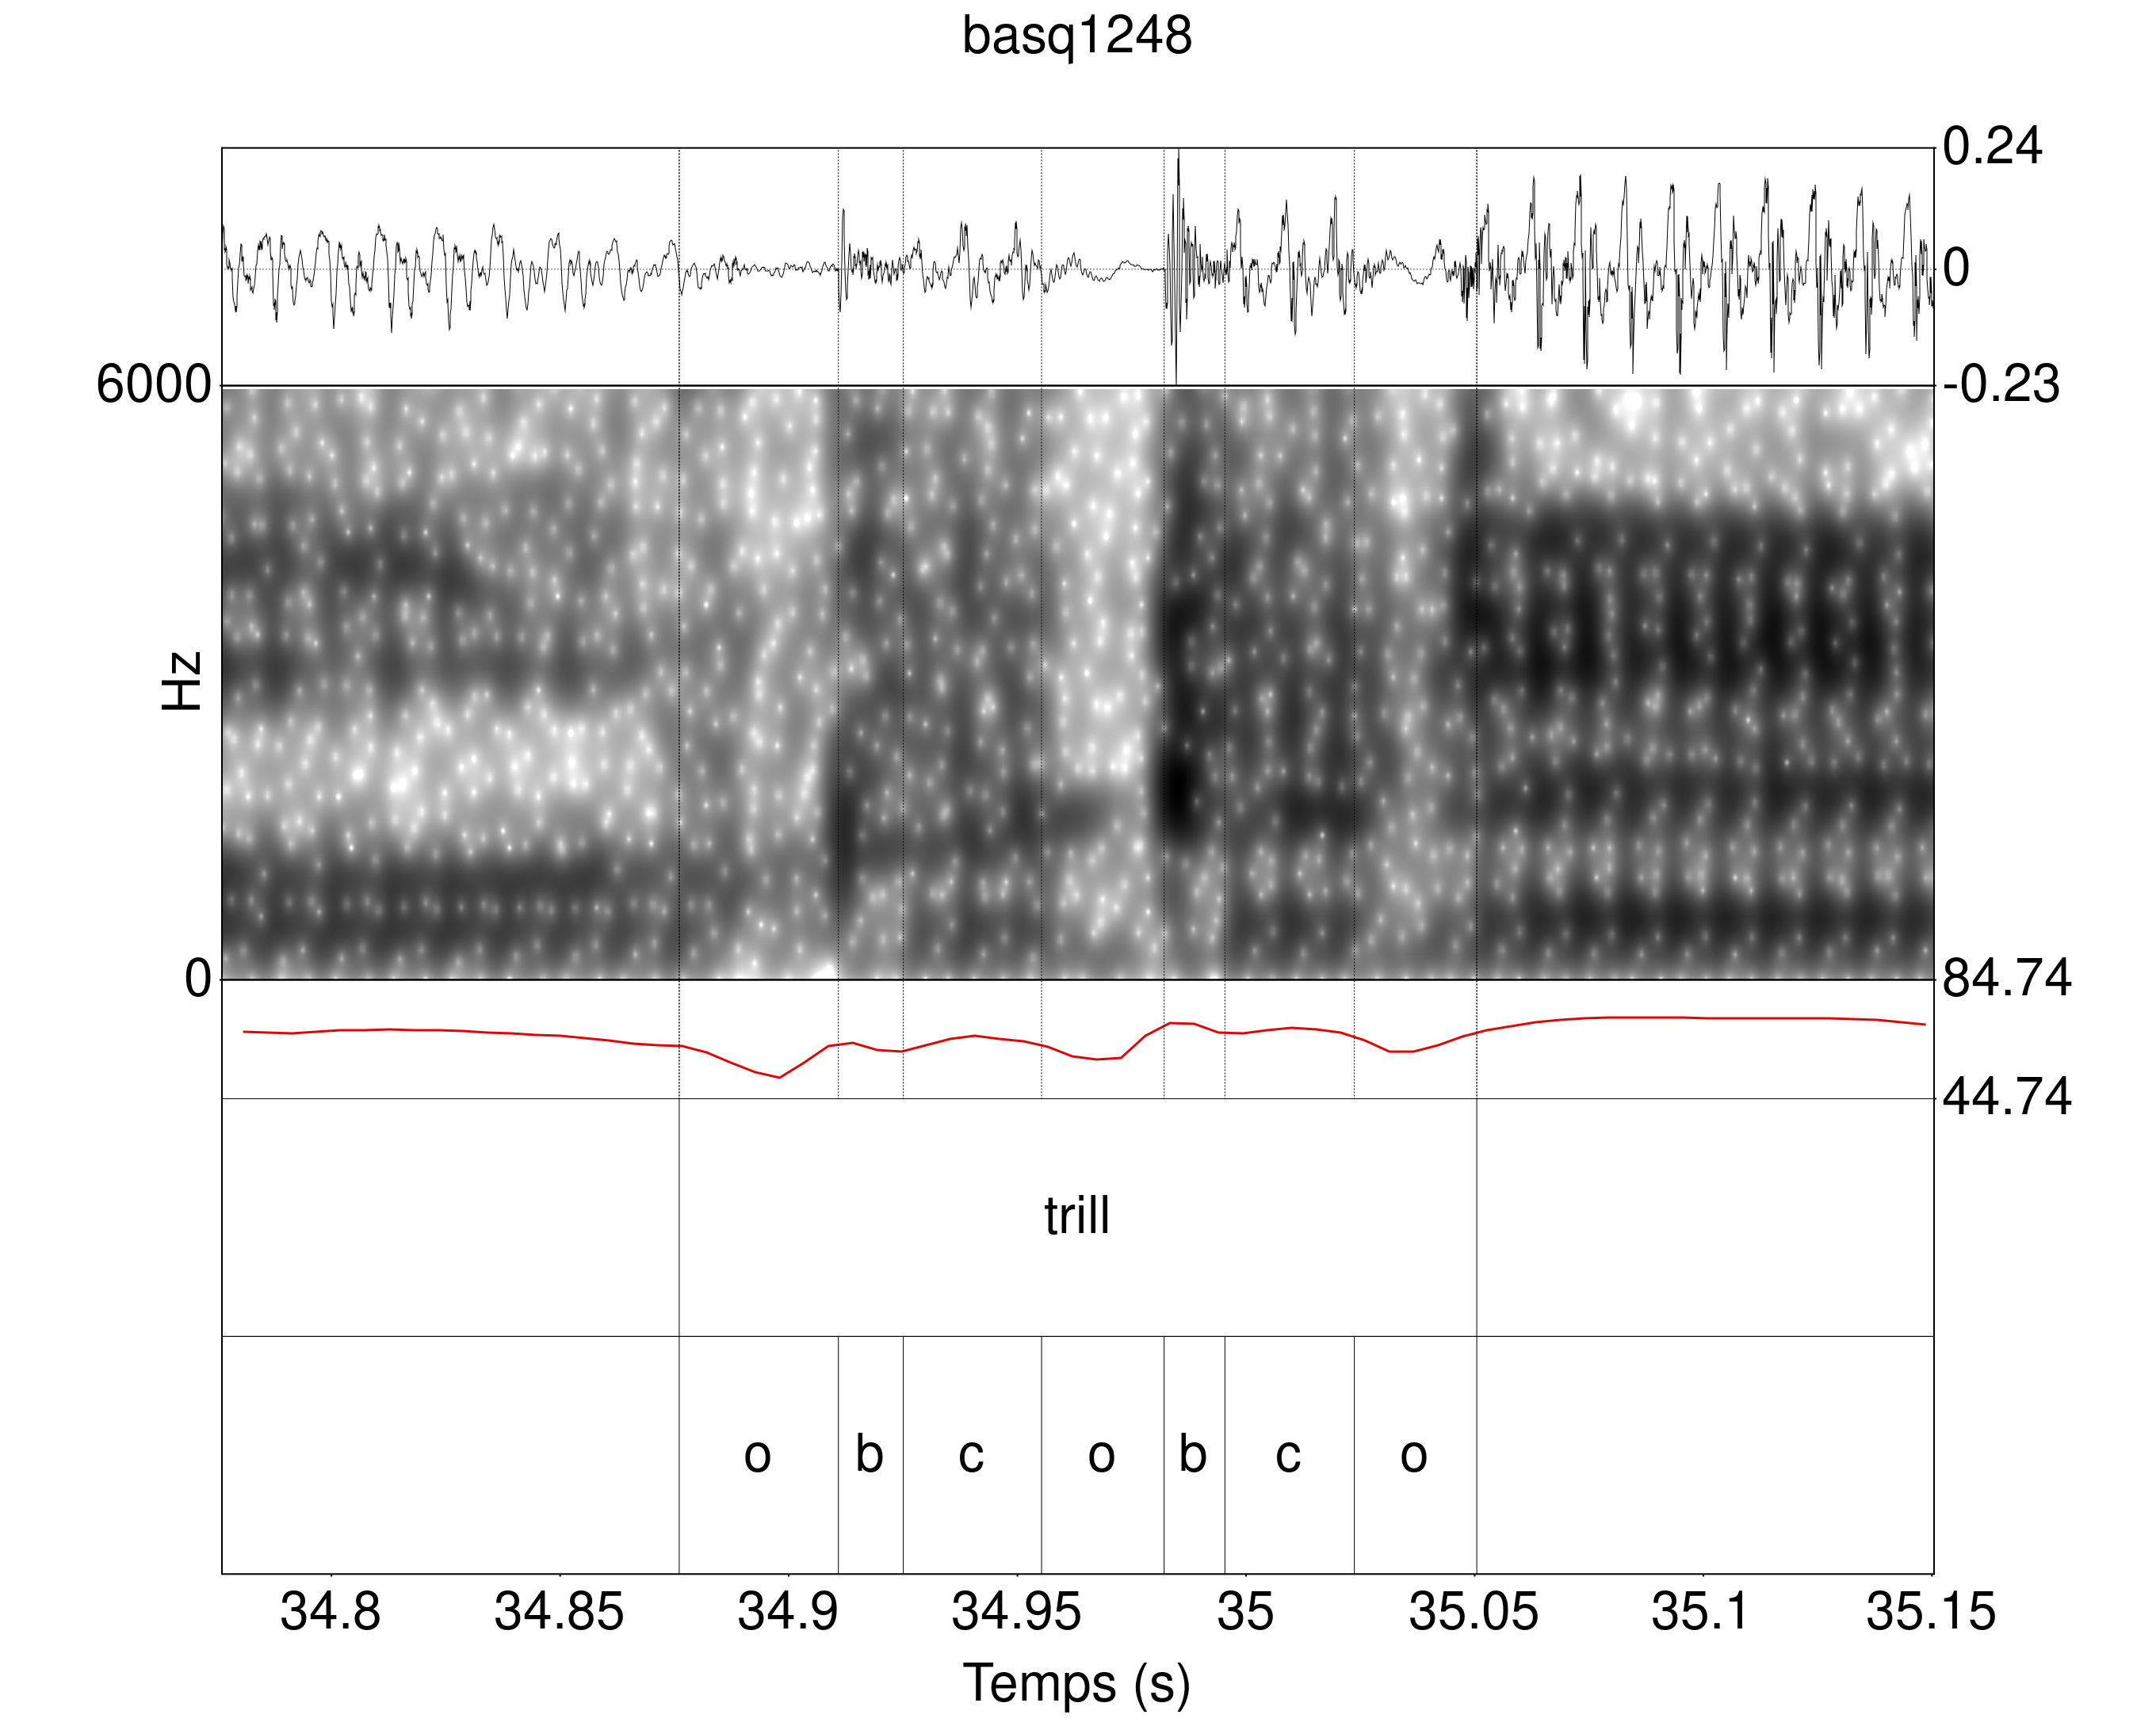
\includegraphics[width=0.7\linewidth]{substance/spectro_images/basq1248_275_ure}
	\caption[Illustration du motif \textg{obcobco}]{Illustration du motif \textg{obcobco} en basque \glotto{basq1248} dans la séquence [ʔau̯réna] orthographiée ‘aurrena’. Il s'agit du seul mot dans la fable écrit avec un <rr>. De haut en bas, nous avons l'oscillogramme, le spectrogramme, la courbe d'intensité, un palier intervallique avec la catégorie segmentée, et un palier intervallique comprenant le label descriptif du segment d'intérêt.}
	\label{fig:basq1248275ure}
\end{figure}


Le motif avec le plus d'éléments est celui \textg{obcobco} avec trois occlusions. Ce motif est illustré en \autoref{fig:basq1248275ure} pour une rhotique du basque. Nous observons dans le segment une succession de plusieurs périodes consécutives constituées de relâchements, d'éléments vocaliques et d'occlusions, avant un [e]. Les occlusions et les relâchements sont caractérisés par une diminution de l'intensité. Les éléments vocaliques sont caractérisés par une augmentation de l'intensité.\\

Dans les motifs à trois occlusions, on retrouve aussi le motif \textg{ococo} (n=3) ainsi que le motif \textg{obobob} (n=1).\\

\begin{figure}
\centering
	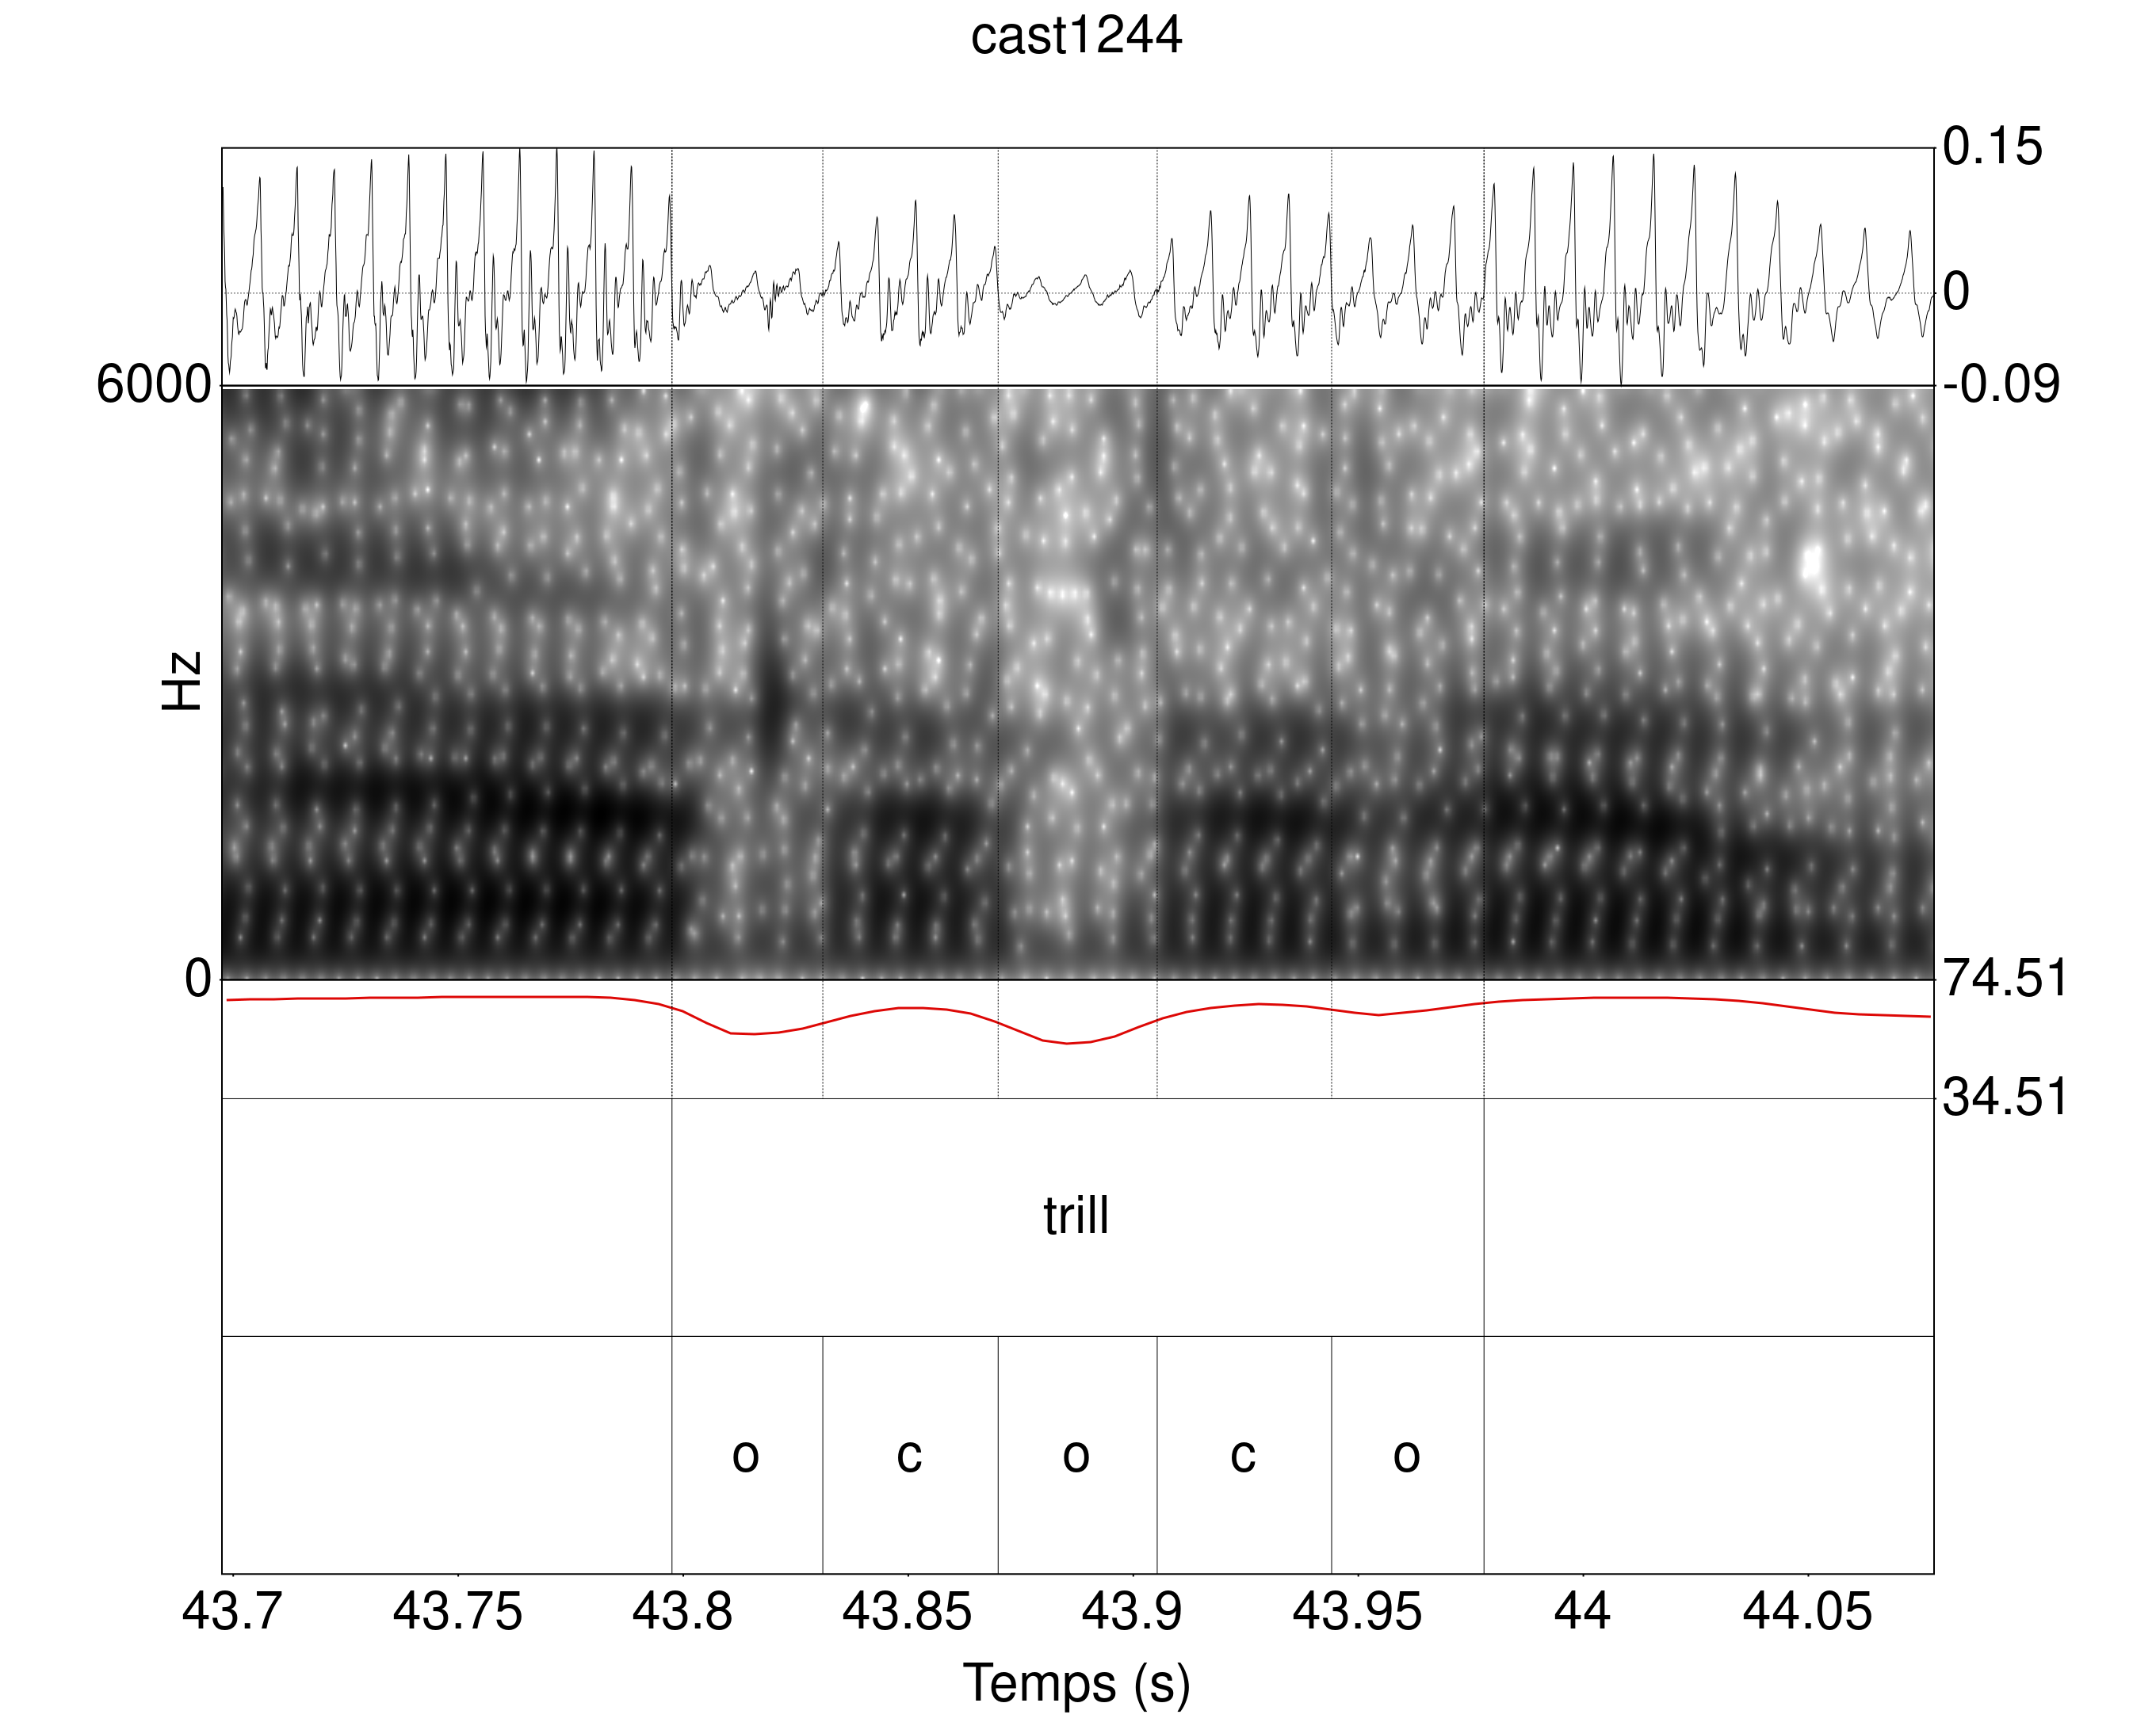
\includegraphics[width=0.7\linewidth]{substance/spectro_images/cast1244_444_are}
	\caption[Illustration du motif \textg{ococo}]{Illustration du motif \textg{ococo} dans le contexte [areβu'xaβa] <arrebujaba> en espagnol castillan \glotto{cast1244}. Nous avons choisi d'annoter le dernier élément \textg{o} et pas \textg{a} à cause de la diminution de l'intensité qui n'est pas aussi marquée que pour les autres éléments \textg{o}. De haut en bas, nous avons l'oscillogramme, le spectrogramme, la courbe d'intensité, un palier intervallique avec la catégorie segmentée, et un palier intervallique comprenant le label descriptif du segment d'intérêt.}
	\label{fig:cast1244444are}
\end{figure}

Le motif \textg{ococo} en \autoref{fig:cast1244444are} est caractérisé par trois occlusions et deux éléments vocaliques intermédiaires.\\

\begin{figure}
	\centering
	\includegraphics[width=0.7\linewidth]{substance/spectro_images/sanm1298_1242_arə}
	\caption[Illustration du motif \textg{obobo}]{Illustration du motif \textg{obobo} dans le contexte [arə] <arrebujaba> en trique d'Intunyoso \glotto{sanm1298}. De haut en bas, nous avons l'oscillogramme, le spectrogramme, la courbe d'intensité, un palier intervallique avec la catégorie segmentée, et un palier intervallique comprenant le label descriptif du segment d'intérêt.}
	\label{fig:sanm12981242ar}
\end{figure}

L'objectif de cette partie était de montrer la diversité qui peut exister dans les différents motifs. La liste de motifs obtenus n'est pas exhaustive. En effet, en segmentant et annotant d'autres enregistrements audios, nous avons eu de nouvelles combinaisons d'éléments comme \textg{obac} dans des contextes VrC\footnote{Nous référons ici aux enregistrements d'une locutrice native du mongol qui ne sont pas inclus dans cette thèse.}. Les motifs obtenus sont, dans une certaine mesure, dépendants des contextes de la fable La Bise et le Soleil.\\

Il n'existe pas une stratégie articulatoire unique pour la production d'un trill ou d'un tap, et cela se reflète dans les acoustiques.
Sur les 400 motifs obtenus, 54 (13,5\%) possèdent au minimum deux éléments \textg{o}. En considérant la possibilité d'avoir aussi des éléments \textg{a}, 100 motifs sur 400 (25\%) possèdent au moins deux éléments qui sont des \textg{a} et/ou \textg{o}. 
Si on considère uniquement les segments ayant un label descriptif \textg{trill}, ce chiffre est de 86 (soit  39,63\% des 217 trills). Pour les \textg{taps}, il existe 13 motifs sur 147 (8,84\%) avec au moins deux éléments qui sont des \textg{a} et/ou \textg{o}.\\

Un motif avec au moins deux contacts (plus ou moins complets, ce qui se traduit par \textg{o} ou \textg{a}) n'est pas fréquent même au sein des segments labellisés comme trill.

\subsection{Les durées des motifs}

\begin{figure}
	\centering
	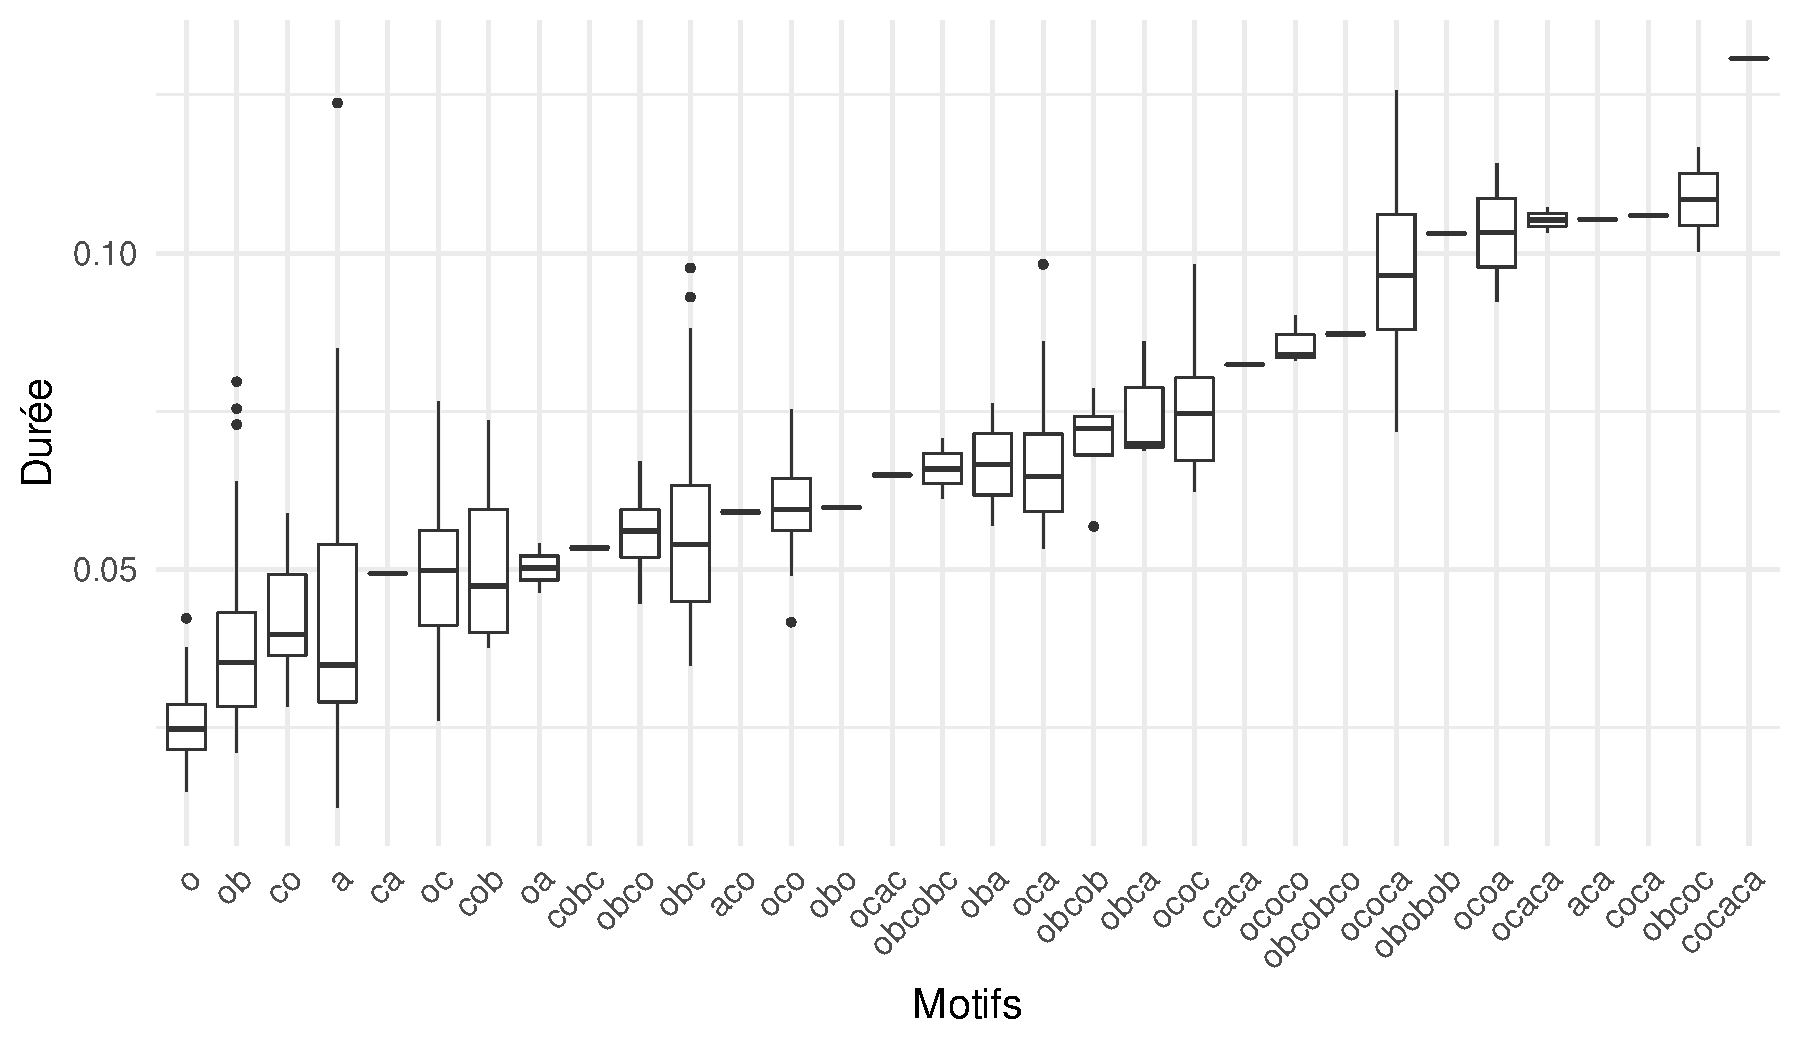
\includegraphics[width=1\linewidth]{substance/images/motifs_duree}
		\caption[La durée en secondes des différents motifs]{La durée en secondes des différents motifs.}
	\label{fig:motifsduree}
\end{figure}

Toutes rhotiques confondues, la durée moyenne était de 48,10 ms, la durée médiane était de 44,72 ms. Le minimum, 12,42 ms, a été obtenu pour le motif \textg{a} et le maximum, 130,77 ms, a été obtenu pour le motif \textg{cocaca} (\autoref{fig:koto_gayo}). L'écart interquartile est de 31,08 ms.
Un test de Kruskal–Wallis permet de mettre en évidence que les différents motifs ont des durées différentes (H(31)=274.4428, p<0.001). Un test post-hoc de Dunn montre cependant que les différences de durée entre les différentes paires ne sont pas toutes significatives. \\

Nous nous intéressons à présent aux dix motifs les plus fréquents.
Le motif \textg{o} a une durée moyenne de 25,53 ms et une médiane de 24,82 ms (maximum à 42,3 ms, minimum à 15,03 ms et IQR de 7,1 ms). Sa durée moyenne est inférieure à celle de tous les autres motifs (p<0.001 dans les neuf cas).
Le motif \textg{a} a une durée moyenne de 44,88 ms et une médiane de 34,94 ms (maximum à 123,70 ms, minimum à 12,41 ms et IQR de 24,82 ms). Le motif \textg{a} n'est significativement différent que de \textg{o}, \textg{oca} et \textg{ococ} (p<0.05 dans les trois cas).
De plus, le test montre que \textg{cob} et \textg{obc}, \textg{obc} et \textg{oco}, et \textg{oca} et \textg{oco} ne sont pas significativement différents. \textg{ob} reste différent de \textg{obc} (p<0.001) mais pas de \textg{oc}. \\

\begin{figure}
	\centering
	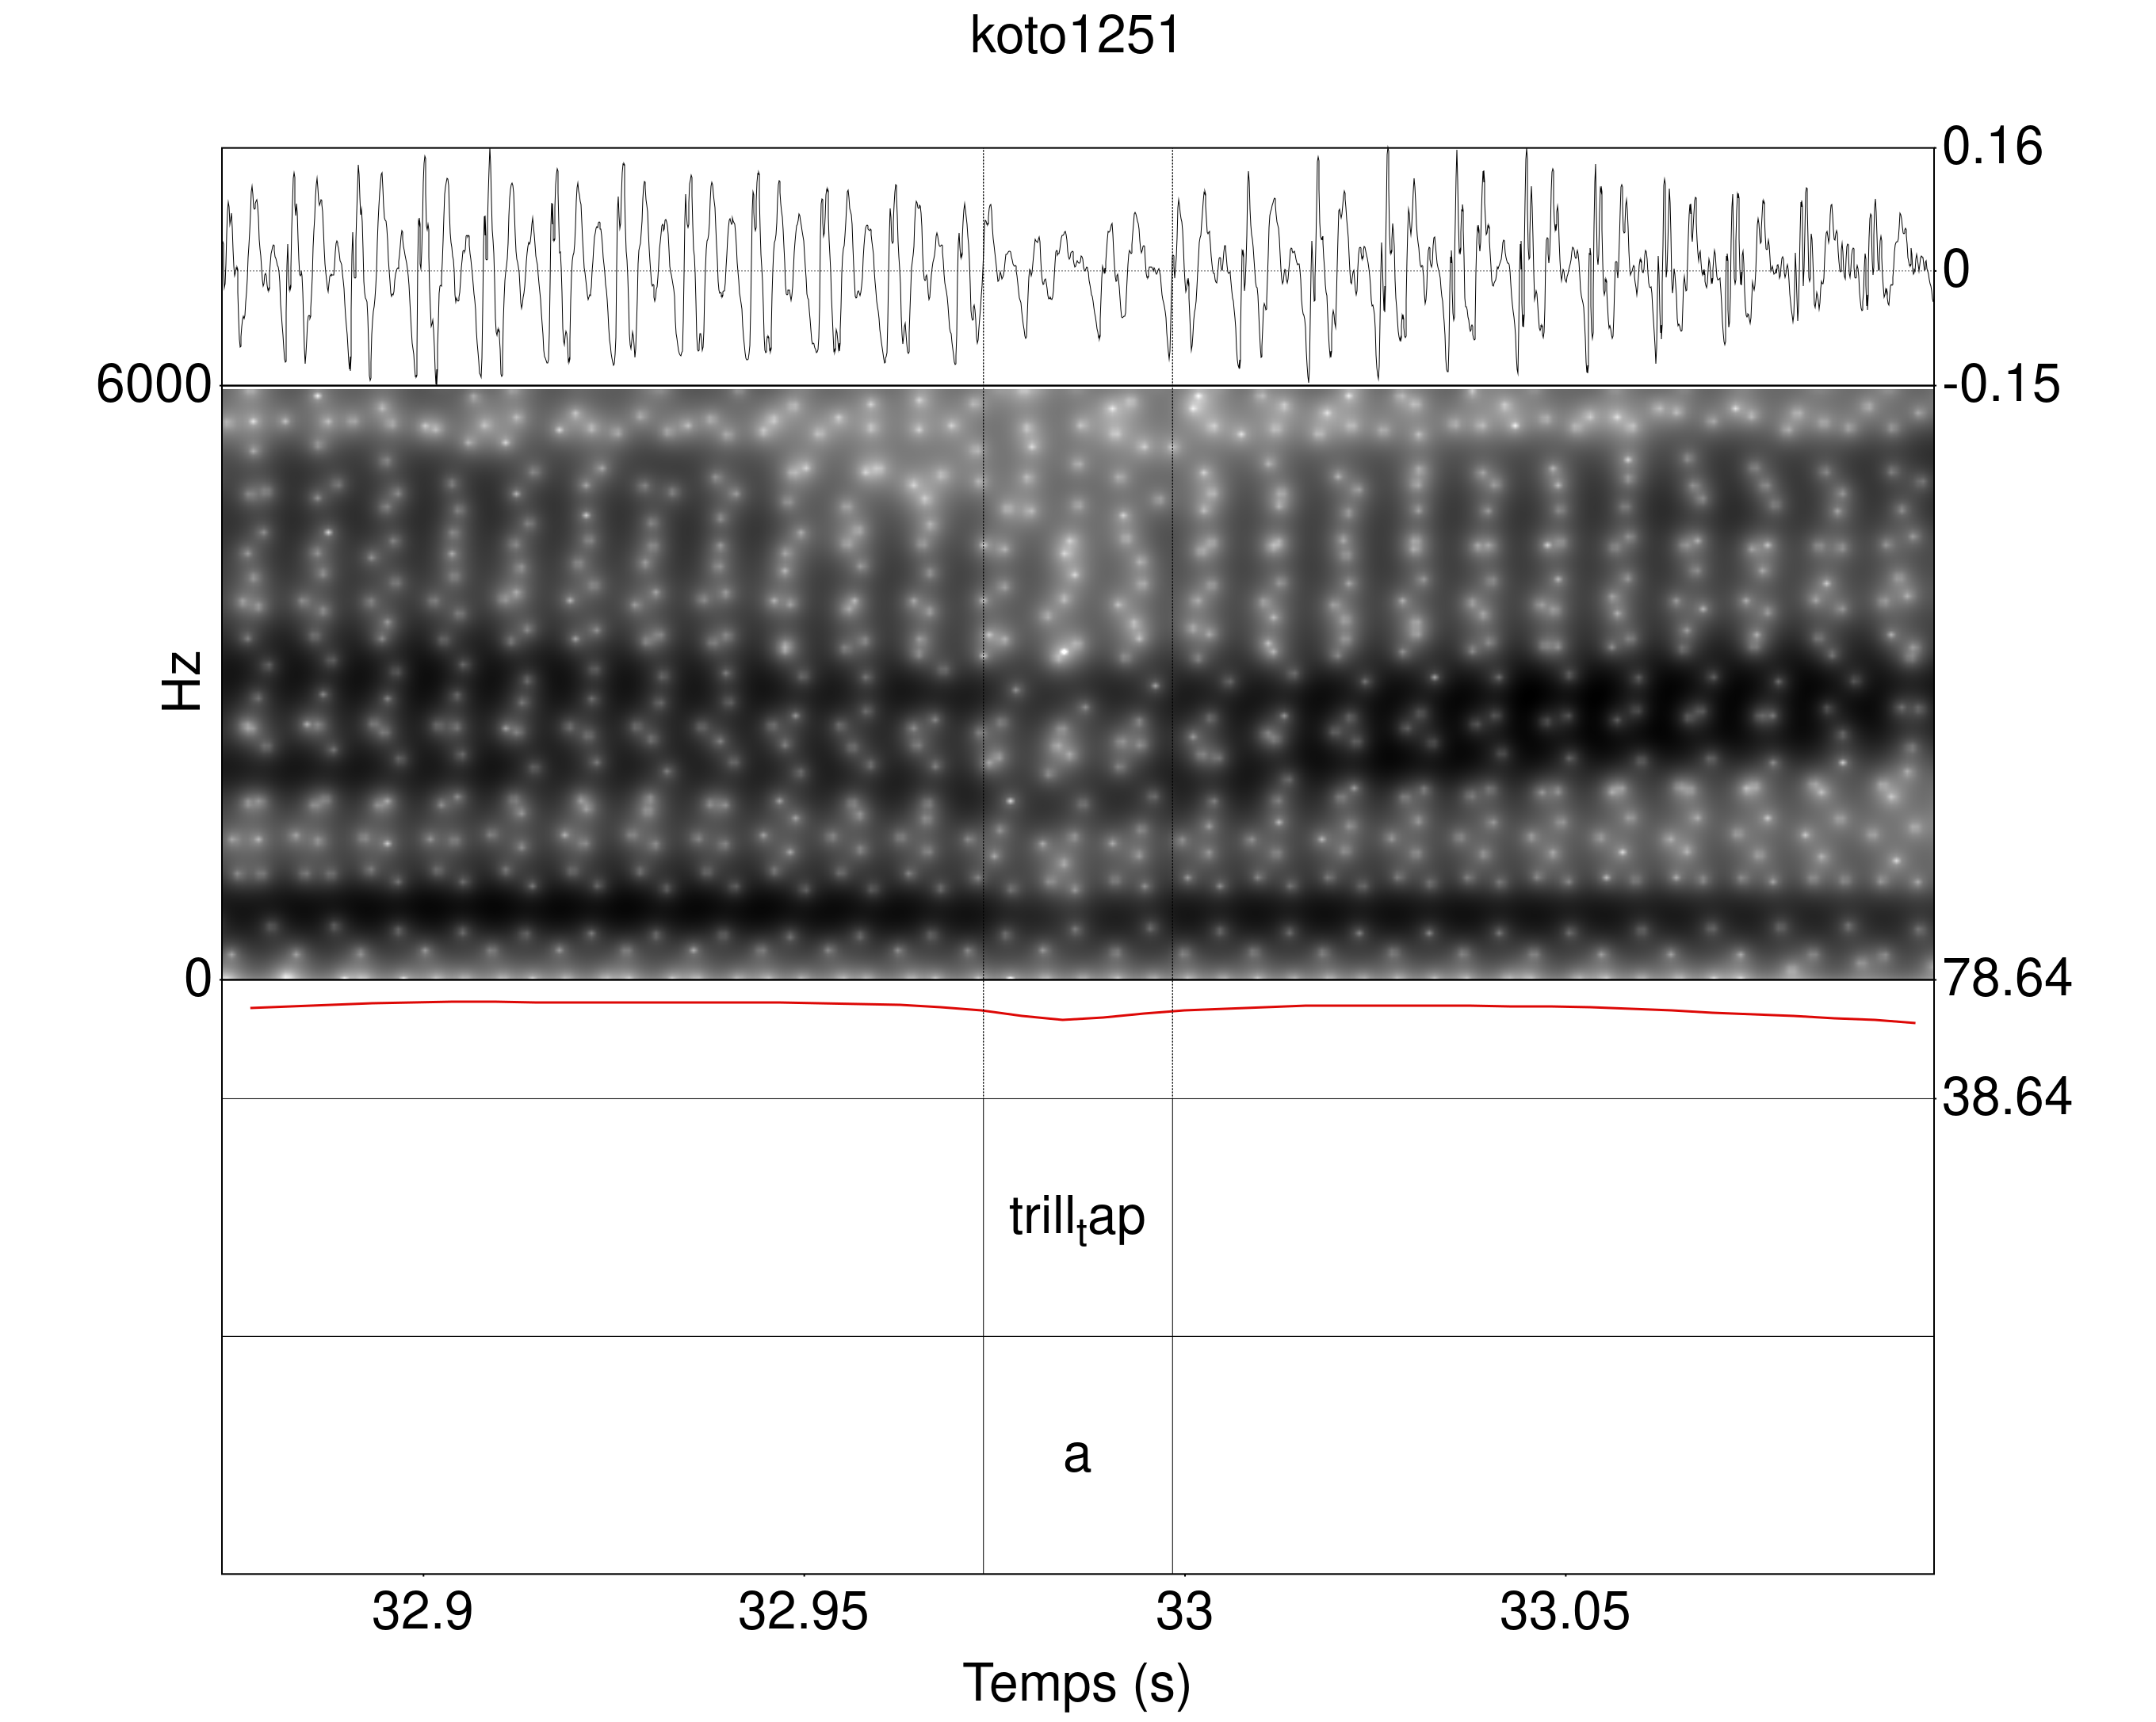
\includegraphics[width=0.45\linewidth]{substance/spectro_images/koto1251_872_ɛrɛ}
	\includegraphics[width=0.45\linewidth]{substance/spectro_images/gayo1244_672_ə}
	\caption[Illustrations des motifs \textg{a} et \textg{cocaca}]{Illustration du motif \textg{a} en amarasi dans le contexte [nɛkmɛsɛ ɾɛʔ] (à gauche) et du motif \textg{cocaca} en gayo dans le contexte [|| rəˈɲəl̪] (à droite). De haut en bas pour chaque illustration, nous avons l'oscillogramme, le spectrogramme, la courbe d'intensité, un palier intervallique avec la catégorie segmentée, et un palier intervallique comprenant le label descriptif du segment d'intérêt.}
	\label{fig:koto_gayo}
\end{figure}

Dans la suite, nous allons uniquement nous intéresser aux éléments \textg{o} dans les neuf motifs les plus fréquents.\\

\begin{figure}
	\centering
	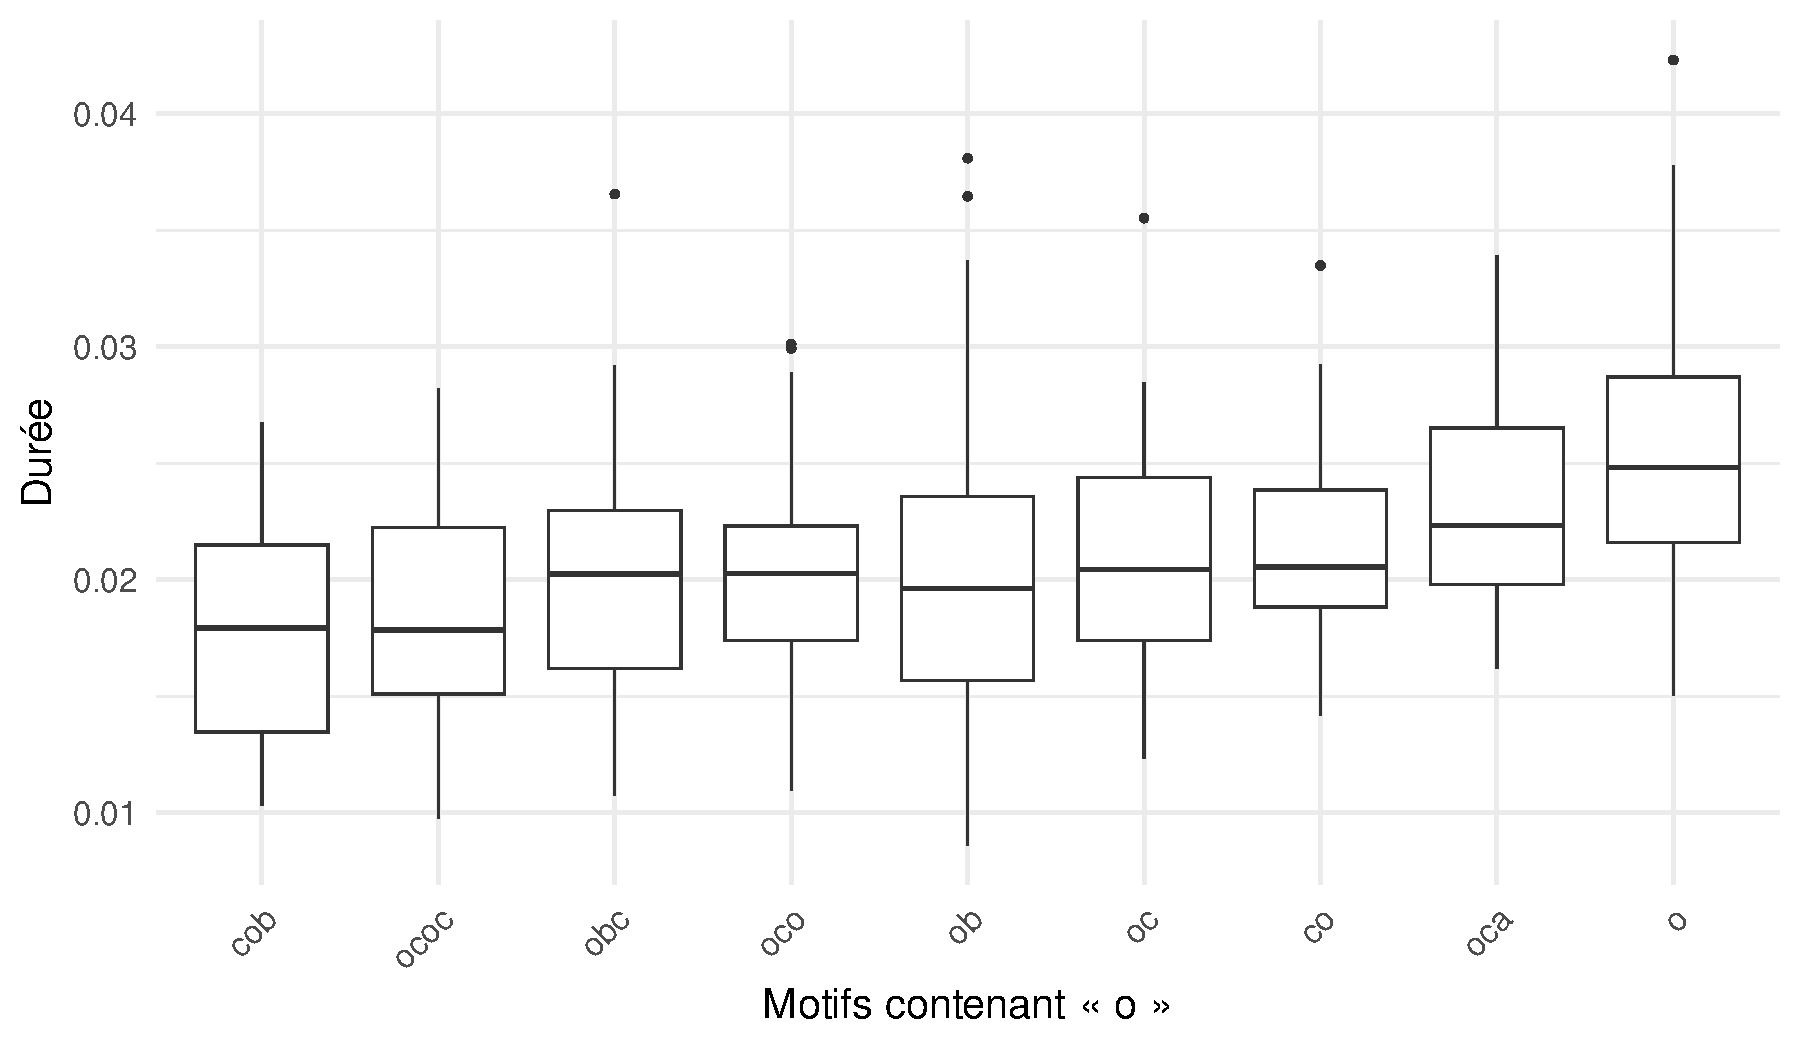
\includegraphics[width=0.7\linewidth]{substance/images/motifs_duree_o}
	\caption[Durées moyennes en secondes des \textg{o} en fonction des motifs les contenant]{Durées moyennes en secondes des \textg{o} en fonction des motifs les contenant. Aucune différence n'est faite entre le premier \textg{o} d'un motif ou le deuxième \textg{o}, bien que la durée de l'élément \textg{o} diminue lorsqu'il est placé plus à droite dans le motif.}
	\label{fig:motifsdureeo}
\end{figure}

Un test de Kruskal–Wallis permet de mettre en évidence que les éléments \textg{o} ont une durée différente en fonction du motif dans lequel ils sont inclus (H(8)=59.9273131, p<0.001). Le test post-hoc de Dunn montre que toutes les différences de durée entre un élément \textg{o} dans un motif \textg{o} et dans un autre motif (comme, par exemple, \textg{oco} ou \textg{obc}) sont significatives (p<0.05) à l'exception de \textg{oca} et de \textg{co}. Autrement dit, les durées des \textg{o} dans les motifs avec plus d'un élément ne sont pas significativement différentes (sauf pour \textg{oca} et \textg{co}).\\

La durée d'un \textg{o} en isolation sans \textg{b} est plus grande que celle d'un \textg{o} dans un motif à plusieurs éléments, comme \textg{oco} pouvant s'interpréter comme deux moyens articulatoires d'obtenir une occlusion. Soit la langue fait un mouvement délibéré, soit la langue fait un mouvement induit par des forces aérodynamiques \parencite{soleAerodynamicCharacteristicsTrills2002}.

\subsection{Les différents contextes possibles}

Travailler sur peu de langues, nous restreint aux contraintes phonotactiques des différentes langues utilisées, en notant également que les langues indo-européennes et austronésiennes sont surreprésentées dans notre échantillon. Ainsi, nos résultats ne représentent que des tendances et ont seulement vocation à être descriptifs.\\

Pour travailler sur les différents contextes, nous avons sélectionné les motifs qui avaient été annotés plus de dix fois. De plus, nous avons sélectionné uniquement des motifs contenant au moins un élément \textg{o}.\\

\begin{figure}
	\centering
	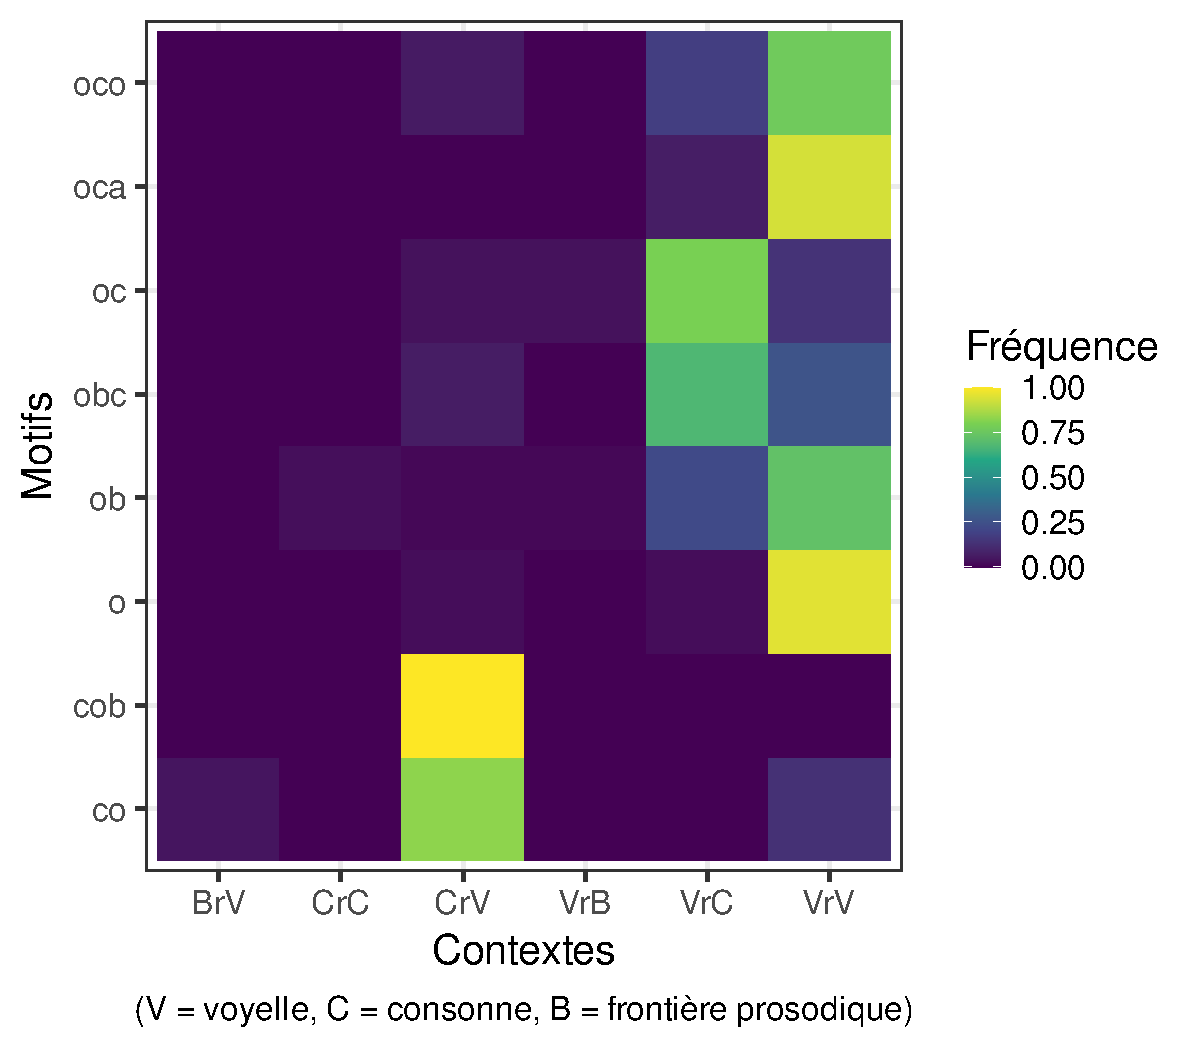
\includegraphics[width=0.45\linewidth]{substance/images/contexte_full}
	\caption[Fréquences des différents motifs en fonction des contextes]{Fréquences des différents motifs en fonction des contextes. Les fréquences sont calculées par ligne. Une case jaune signifie qu'un motif est intégralement trouvé dans un seul contexte, une case violette signifie qu'un motif n'est pas présent dans ce contexte.}
	\label{fig:contextefull}
\end{figure}

En \autoref{fig:contextefull} nous pouvons observer que les motifs se retrouvent principalement dans deux contextes : le contexte intervocalique et le contexte post-vocalique pré-consonantique. 
Les motifs avec un élément vocalique servant de transition entre la consonne et l'occlusion, entre ou l'occlusion et la consonne diffèrent. En effet, les motifs \textg{cob} et \textg{co} se retrouvent principalement en position post-consonantique pré-vocalique. Les consonnes pré-occlusion comprennent [p β d t ð g k ɣ]. Les motifs \textg{oc} et \textg{obc} se retrouvent principalement en position post-vocalique et pré-consonantique. Les consonnes post-occlusion, quant à elles, comprennent les sons suivants : [b v f ʋ n t d ð l j g k ɦ].\\

Pour le contexte intervocalique, indépendamment du motif, on retrouve une multitude de voyelles avant le motif [a ɐ ɑ e ə ɛ i ɪ o ɔ u ṵ ɯ ʊ y]. Le [a] représente 31,93\% des occurrences, suivi du [e] (15,71\%), du [ə] (11,52\%) et du [i] (11\%). Après les motifs, on retrouve [a ɐ ɑ e ə ɛ i ɪ ɨ o ɔ u ɯ ʊ] avec le [a] qui représente 24,61\% des occurrences, le [i] 17,28\% des occurrences et le [o] et le [u] représentent chacun 13,1\%.\\

Enfin, l'élément \textg{b} en position finale d'un motif se retrouve principalement en position intervocalique (60,46\%), en position post-vocalique pré-consonantique (18,6\%) et post-consonantique pré-vocalique (17,44\%). Nous pouvons observer que dans 16,28\% des cas, le \textg{b} était suivi d'un [a] et dans 16,28\% d'un [i].\\

Les contextes varient donc en fonction des motifs segmentés mais restent majoritairement vocaliques. Les frontières prosodiques sont peu présentes dans notre corpus, ceci étant dû au style d'élicitation des données (et au style de transcription des auteurs/trices). Nous n'avons donc pas l'opportunité d'observer beaucoup de motifs dans ces positions.

\section{Discussion}


	
Notre chapitre acoustique se fonde sur deux études utilisant deux méthodologies différentes. La première méthodologie s'appuie sur l'annotation de motifs dans le signal acoustique à travers des catégories suffisamment larges pour pouvoir être flexibles et s'appliquer à 73 langues. Nous avons souhaité capturer des caractéristiques invariantes dans les différentes rhotiques. 
La deuxième méthodologie repose sur une analyse plus fine du signal acoustique. Au lieu des catégories de la première étude, la deuxième étude parle d'éléments. La combinaison de ces éléments donne lieu à des motifs. Ces deux méthodologies sont résumées et schématisées dans la \autoref{fig:schemarecapacoustics}. Ce qui est intéressant c'est que l'interprétation des motifs, qu'elle soit au niveau des catégories ou de la combinaison d'éléments, donne lieu à différentes dénominations par les auteurs et autrices qui ont publié une \textit{Illustration of the IPA}. Le \textg{trill}, de même que le \textg{tap} et le \textg{flap}, peuvent être réalisés comme un \textg{t1} ou un \textg{t2}, bien que la réalisation \textg{t2} soit moins fréquente pour les labels descriptifs \textg{tap} et \textg{flap}. Lorsque ces segments sont réalisés comme des \textg{t2}, l'analyse en élément nous permet de voir qu'il n'existe pas qu'une interprétation de ce que contient un \textg{t2}.\\ 

De plus, les deux études permettent de mettre en avant que la catégorie \textg{t2}, qui correspondrait à un trill à au moins deux occlusions, n'est pas la plus fréquente.
En effet, avec la deuxième étude, nous avons pu observer que les segments à plusieurs éléments \textg{o} ou \textg{a} n'étaient pas fréquents. Ces résultats viennent ainsi conforter ceux de \textcite{lindauStory1985}.\\

Ce chapitre s'intéresse aux rhotiques produites dans des textes. Pour autant il reste à vérifier si les méthodologies utilisées peuvent s'appliquer aussi à d'autres méthodes d'élicitation de données. Nous avons commencé à travailler sur les listes de mots avec la première méthode, celle des quatre catégories, mais nous n'avons pas continué tant la variation dans les productions était importante. Quatre catégories (ou six) ne nous semblaient pas suffisantes. Il nous aurait fallu une vision globale des données, vision que nous n'avions pas. Il faudrait donc voir si la deuxième méthodologie rend mieux compte de la variation dans les sons \textg{simil-\textit{r}} dans les listes de mots.
Finalement, il nous parait important d'avoir une méthodologie robuste pour la segmentation et l'annotation des rhotiques pour pouvoir faire des études comparatives entre plusieurs langues. Nous pourrions potentiellement étendre ces méthodes à l'étude des trills chez les locuteurs/trices qui ne sont pas capables de triller, et dans d'autres espèces animales où on retrouve une modulation du signal similaire à celle des trills humains.

\newgeometry{inner=3.31cm,outer=3.81cm}
\begin{landscape}
	\begin{figure}
		\centering
		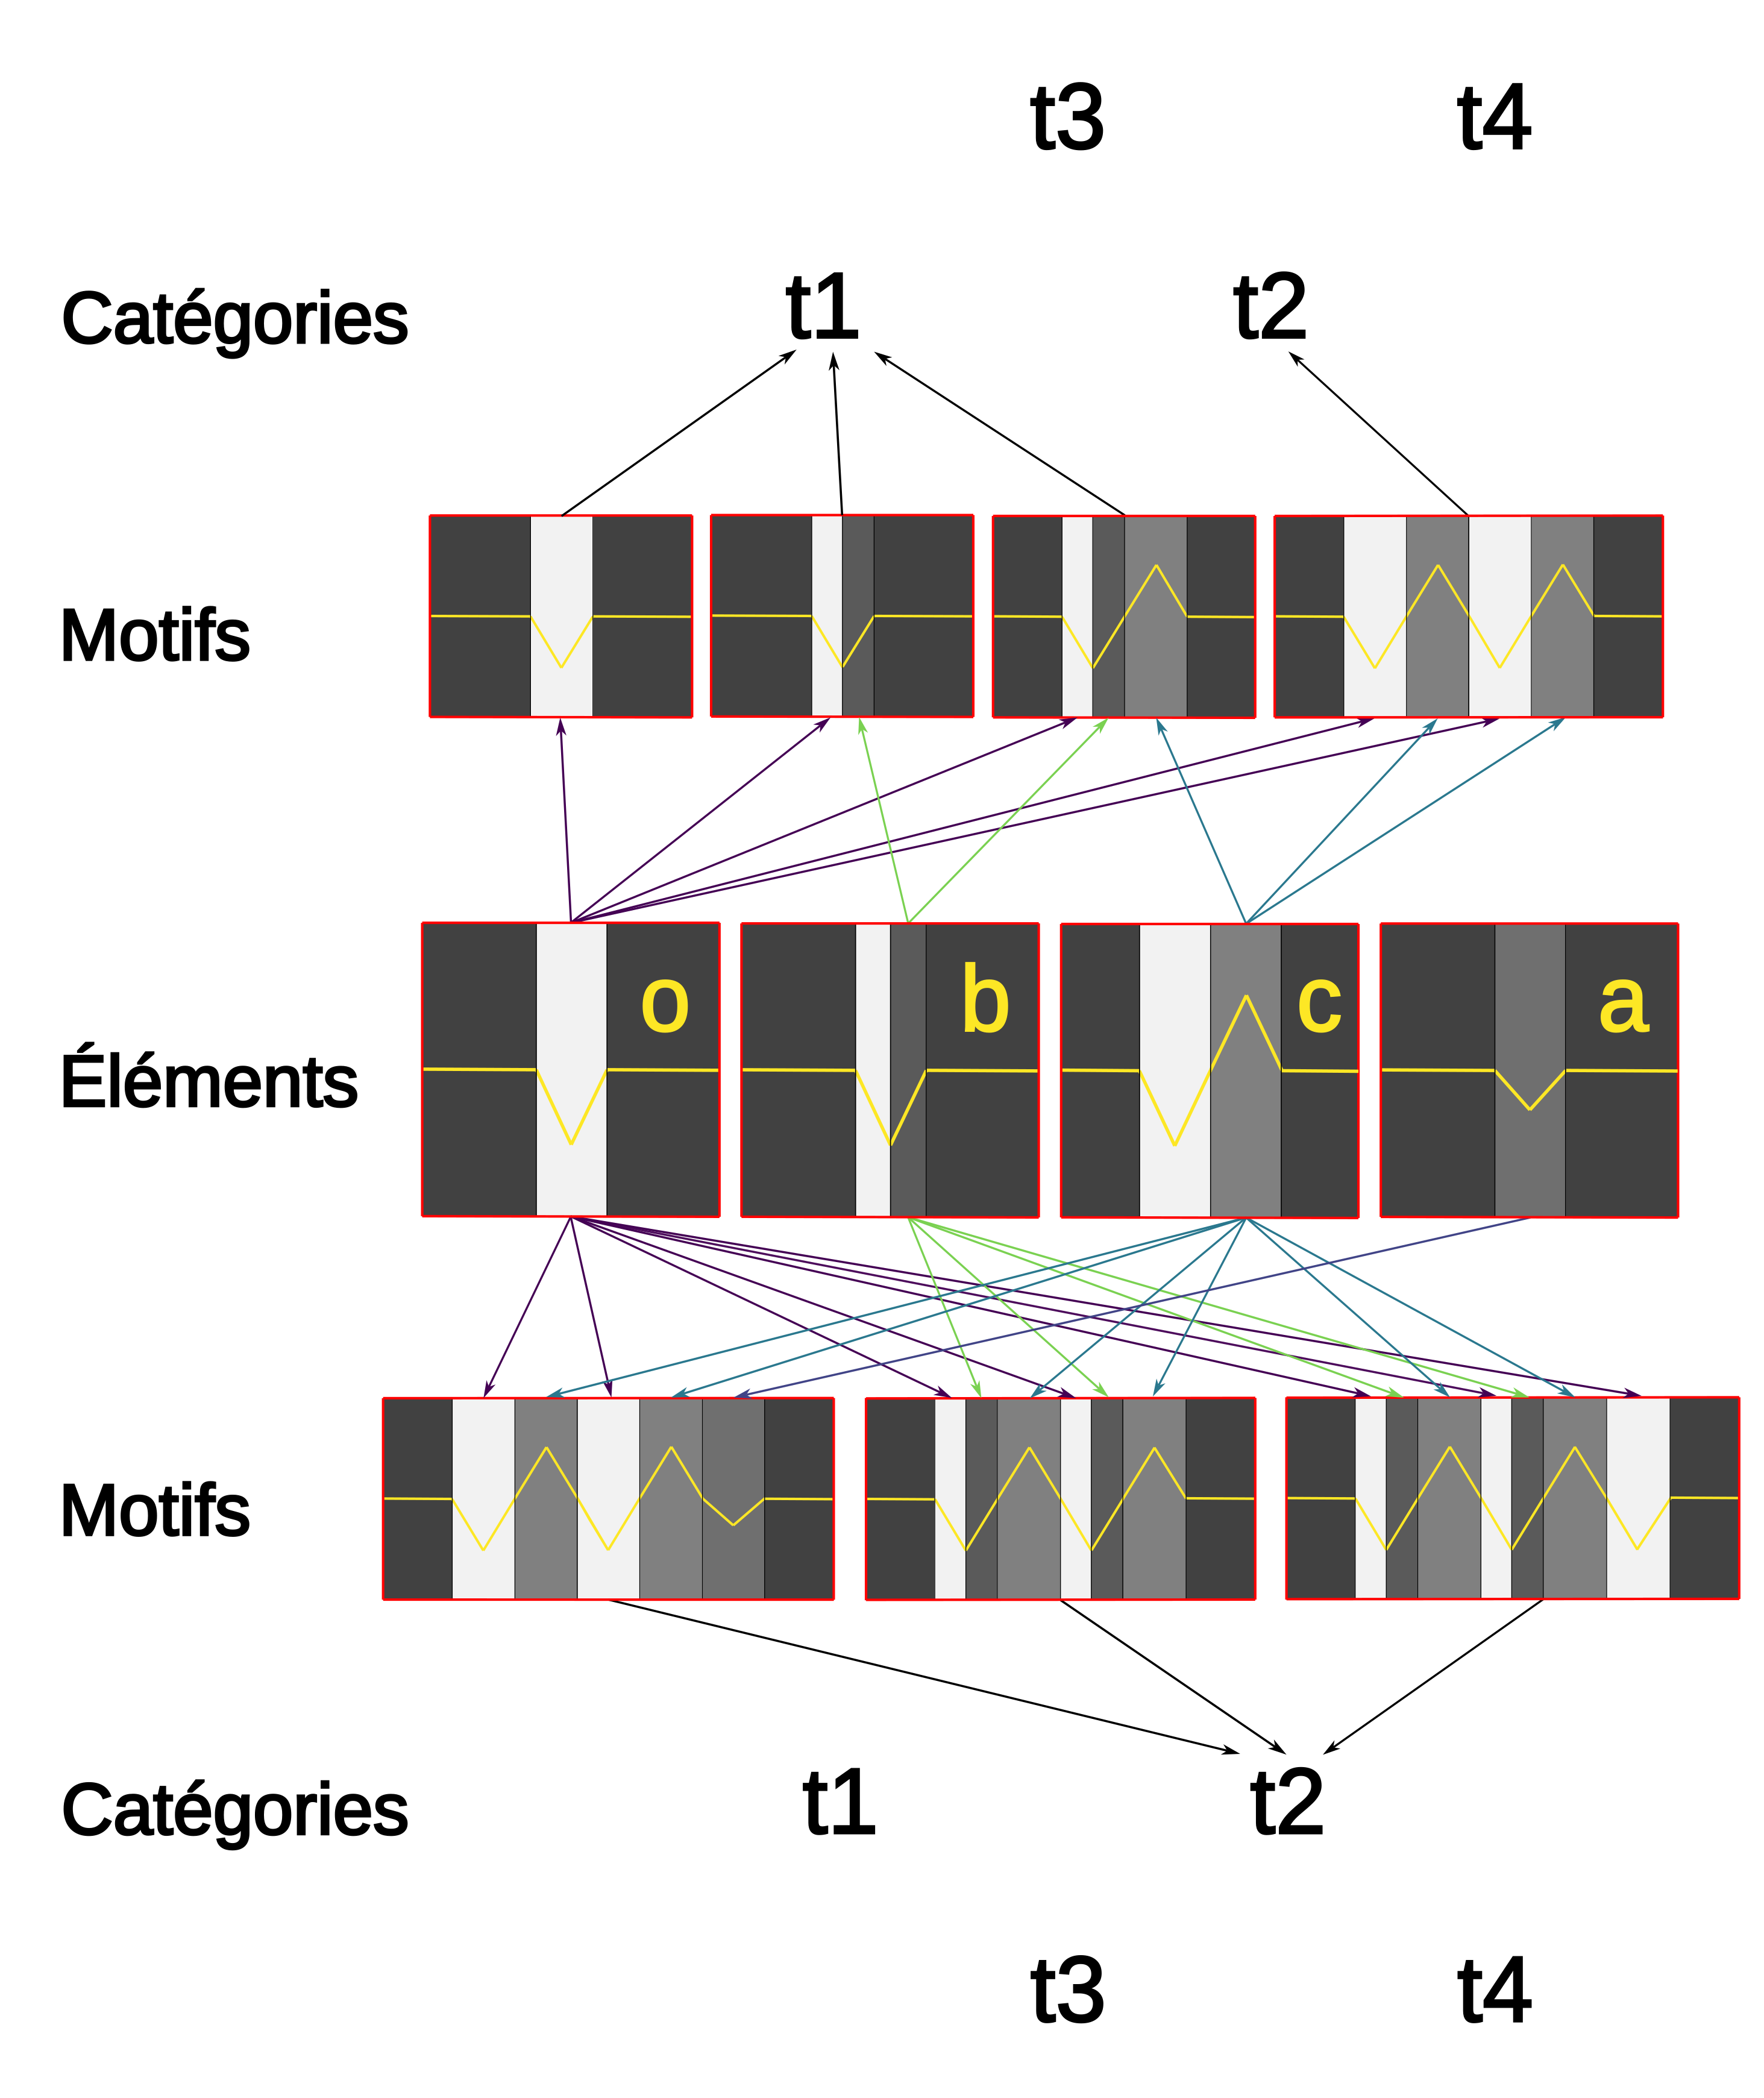
\includegraphics[width=0.5\linewidth]{substance/images/schema_test}
		\caption[Schéma récapitulatif des méthodes utilisées pour la représentation du <r> en acoustique]{Schéma récapitulatif des méthodes utilisées pour la représentation du <r> en acoustique. Les éléments sont l'unité minimale que nous avons segmentée. Nous avons schématisé la représentation spectrographique des éléments \textg{o}, \textg{b}, \textg{c}, et \textg{a} avec la variation de l'intensité (représentée en jaune). Le contexte qui peut être vocalique ou consonantique est représenté en gris foncé. Les éléments peuvent se combiner pour former des motifs, c'est ce qui est observable au niveau du signal acoustique (également schématisé avec une représentation spectrographique et la courbe d'intensité). Nous avons choisi les motifs les plus fréquents composés de un à sept éléments. Sans passer par la segmentation fine des différents éléments, il est possible d'établir des catégories regroupant un ensemble de patrons au niveau du signal acoustique.}
		\label{fig:schemarecapacoustics}
	\end{figure}
\end{landscape}
\restoregeometry